\chapter[Topological and Optical Properties of Beryllene Phases]{Emergent Topological and Optical Properties in Pristine and Hydrogen-Functionalized Two-Dimensional Beryllium Phases}
\label{cha:project_beryllene}

\section{Abstract}
\label{3_abstract}

Two-dimensional elemental materials provide a direct platform for exploring electronic,
optical,
and topological phenomena arising from reduced dimensionality and modified bonding environments.
In this chapter,
we use density functional theory calculations to investigate the structural stability,
electronic structure,
optical response,
and topological characteristics of pristine and hydrogen-functionalized beryllene systems.
The structures considered include monolayer $\alpha$-beryllene,
bilayer $\beta$-beryllene,
bulk reference phases,
and newly identified trilayer cubic beryllene,
an ABA-stacked trilayer beryllene with a square lattice.
In addition to confirming the stability of previously proposed $\alpha$- and $\beta$-beryllene phases,
we predict a dynamically stable trilayer cubic beryllene phase with distinct electronic and optical characteristics.
Hydrogen functionalization drives $\alpha$-beryllene into a wide-gap semiconducting state with an HSE06 band gap of \qty{6.00}{\electronvolt},
whereas the hydrogen-functionalized $\beta$-based structures remain metallic,
and only hydrogenated $\alpha$-beryllene is thermodynamically stable against \ce{H2} release under ambient conditions.
The calculated dielectric response reveals strong anisotropy and low-dimensional optical effects,
including a direction-dependent redistribution of visible-to-ultraviolet optical response
and distinct dielectric and energy-loss features under the stated effective-thickness convention.
Furthermore,
parity analysis of the spin-orbit-coupled electronic states shows that,
beyond $\alpha$-beryllene,
trilayer cubic beryllene also has a non-trivial $Z_{2}$ invariant for its lowest six bands,
which are isolated only by spin-orbit gaps of approximately \qty{1}{\milli\electronvolt} above the Fermi level,
whereas all hydrogen-functionalized structures are trivial.
These results identify beryllene as an elemental two-dimensional platform that combines metallicity,
tuneable optical properties,
and non-trivial topology.

\section{Introduction}
\label{3_introduction}

Two-dimensional materials have reshaped modern materials science by enabling access to electronic,
thermal,
and mechanical properties that differ substantially from those of their bulk counterparts.
Since the isolation of graphene,
reduced dimensionality has been shown to give rise to Dirac fermions,
enhanced carrier mobility,
strong many-body interactions,
tuneable band structures,
and anomalous phonon transport~\cite{novoselov2004electric,geim2007rise}.
These effects support rapid progress in nanoelectronics,
optoelectronics,
sensing,
thermal management,
and quantum technologies.

Beyond graphene,
the discovery and prediction of atomically thin materials has expanded to include transition-metal dichalcogenides,
hexagonal boron nitride,
black phosphorus,
and elemental two-dimensional materials,
commonly referred to as Xenes~\cite{butler2013progress,molle2018silicene}.
Elemental two-dimensional materials are particularly attractive because their chemically simple nature allows intrinsic structure-property relationships to be studied without the complexity introduced by multicomponent bonding.
However,
most experimentally realized Xenes are composed of relatively heavy elements,
where strong spin-orbit coupling,
substrate effects,
or structural buckling dominate the physics and may obscure low-energy electronic behaviour.

In contrast,
beryllium represents an extreme and largely unexplored limit within the family of elemental two-dimensional materials.
As the lightest alkaline-earth metal,
bulk beryllium exhibits a unique combination of low density,
high elastic modulus,
high thermal conductivity,
and transparency to X-rays and neutrons.
These properties have led to its use in aerospace,
nuclear,
and optical applications~\cite{zheng2020progress}.
Extending elemental beryllium into the two-dimensional limit raises the prospect of ultralight metallic layers with unconventional electronic and thermal properties governed by reduced dimensionality and strong confinement.

First-principles studies predicted that atomically thin beryllium could exist in metastable hexagonal or stable two-layer hexagonal lattice configurations~\cite{ono2020dynamical,hess2022periodicity}.
However,
for many years,
two-dimensional beryllium remained a theoretical construct due to experimental challenges associated with synthesis and handling.
This situation changed recently with the experimental realization of two-dimensional beryllium,
termed beryllene.
Chahal \textit{et al.} reported the first experimental synthesis and characterization of beryllene using a sonochemical exfoliation approach starting from elemental beryllium powder~\cite{chahal2023beryllene}.
High-resolution transmission electron microscopy revealed atomically thin sheets with multiple structural motifs,
including hexagonal and square-like lattice geometries.
Raman spectroscopy and electron diffraction confirmed crystallinity,
while electrical measurements demonstrated intrinsic metallic conductivity.

Subsequent theoretical investigations have uncovered striking thermal transport behaviour in hexagonal monolayer beryllene.
Using first-principles phonon calculations combined with the Boltzmann transport equation,
Chowdhury and Mogurampelly predicted an exceptionally high in-plane lattice thermal conductivity of approximately \qty{270}{\watt\per\metre\per\kelvin} at room temperature,
which exceeds that of bulk beryllium~\cite{chowdhury2024unusual}.
This enhancement was attributed to suppressed phonon-phonon scattering and the dominant contribution of long-wavelength flexural phonons,
a feature rarely observed in atomically thin metallic systems.
These results suggest that two-dimensional beryllium could serve as an efficient heat-spreading material in nanoscale electronic architectures.

Beyond thermal properties,
the electronic structure of beryllene has been predicted to host non-trivial quantum features.
Several density functional theory studies have identified Dirac-like band crossings near the Fermi level in hexagonal monolayer and bilayer beryllene,
usually denoted as $\alpha$- and $\beta$-beryllene,
arising from symmetry-protected $s$-$p$ orbital hybridization~\cite{li2023coexistence}.
Electron-phonon coupling calculations further suggest that these phases may support phonon-mediated superconductivity with critical temperatures on the order of \qty{10}{K}.
The coexistence of Dirac fermions and superconductivity in an ultralight elemental monolayer distinguishes beryllene from both graphene and heavier Xenes,
and highlights its potential as a platform for low-dimensional quantum phenomena.

The possibility of topological behaviour in two-dimensional beryllium has also been explored from a more fundamental perspective.
Derriche \textit{et al.} demonstrated that light-element lattices dominated by charge-based interactions can host topologically protected electronic states even in the absence of strong spin-orbit coupling~\cite{derriche2024light}.
These findings suggest that beryllene may realize topological phases driven mainly by lattice symmetry and orbital physics,
offering an alternative route to low-dissipation electronic states without relying on heavy elements.
While experimental studies of beryllene remain limited,
earlier work on ultrathin beryllium films and nanostructures has revealed unconventional quantum transport behaviour,
including strong disorder effects and superconducting correlations at low temperatures~\cite{xiong2009spin}.

Two-dimensional topological materials are considered promising for quantum and electronic technologies because their non-trivial band topology gives rise to robust,
symmetry-protected edge states that resist disorder and backscattering~\cite{weber2024roadmap}.
Recent density functional theory studies have shown that simple elemental two-dimensional systems can host switchable or adsorbate-induced topological behaviour.
For example,
interlayer sliding in bilayer elemental bismuth was predicted to switch the system between topologically trivial and non-trivial phases~\cite{qian2025switchable}.
Similarly,
hydrogenation and strain can tune monolayer arsenene into a quantum spin Hall state with a sizable band gap~\cite{zhang2016controllable}.
These studies indicate that structural control and adsorbate functionalization can provide practical routes to topological phases in elemental two-dimensional materials.

Although two-dimensional elemental beryllium has recently been realized experimentally and shown to exhibit unusual electronic and thermal properties,
its interaction with hydrogen has received much less attention.
First-principles investigations of hydrogen adsorption on low-index hexagonal close-packed beryllium surfaces,
particularly Be(0001),
show that hydrogen binds preferentially to high-symmetry adsorption sites with moderate binding energies and induces appreciable local lattice relaxation~\cite{bachurin2015ab}.
These results indicate that beryllium-hydrogen interactions occupy an intermediate regime between weak physisorption and strong ionic hydride formation.
In the two-dimensional limit,
reduced coordination and enhanced lattice flexibility are expected to modify this balance,
potentially stabilizing adsorption geometries or electronic reconstructions that are inaccessible on bulk surfaces.
Using global structure search and density functional theory calculations,
two stable beryllium hydride monolayers were predicted with multicentre beryllium-hydrogen bonding motifs and wide band gaps~\cite{li2018global}.
Although such systems correspond to compound formation rather than surface termination,
they demonstrate that hydrogen can strongly reshape bonding and electronic behaviour in low-dimensional beryllium-based systems.

In this chapter,
we use density functional theory calculations to investigate the atomic,
electronic,
optical,
and topological properties of pristine and hydrogen-functionalized beryllene systems.
In addition to $\alpha$- and $\beta$-beryllene,
the pristine structures include trilayer cubic beryllene,
by which we denote ABA-stacked trilayer beryllene with a square lattice.
The hydrogen-functionalized structures are double-sided hydrogen-terminated $\alpha$-beryllene (2H-$\alpha$-beryllene)
and single-sided and double-sided hydrogen-terminated $\beta$-beryllene (1H-$\beta$-beryllene and 2H-$\beta$-beryllene).
The results identify dynamically stable hydrogen-functionalized structures and a trilayer cubic beryllene phase with a non-trivial $Z_{2}$ index for an isolated band subspace.
The optical properties demonstrate direction-dependent and dimensionality-dependent response,
together with anisotropic dielectric and energy-loss spectra and a redistribution of visible-to-ultraviolet optical response.

\section{Computation methods}
\label{3_methods}

The density functional theory calculations are performed using the Vienna Ab initio Simulation Package,
VASP~\cite{kresse1993ab,kresse1994ab,kresse1996efficiency,kresse1996efficient}.
The projector augmented wave method is used to describe the electron-ion interactions~\cite{kresse1999ultrasoft}.
The generalized gradient approximation of Perdew--Burke--Ernzerhof is employed for the exchange-correlation functional~\cite{perdew1996generalized}.
The structural relaxations,
total energies,
phonon calculations,
and molecular dynamics simulations are performed without a dispersion correction.
The D3 dispersion correction with Becke--Johnson damping~\cite{becke2005density,grimme2010consistent,grimme2011effect} is included in the PBE band-structure calculations without spin-orbit coupling,
where it adds only an energy correction and does not change the Kohn--Sham eigenvalues at the fixed relaxed geometries.
The PBE band structures are calculated non-self-consistently from the self-consistent charge densities,
and their energies are given relative to the Fermi level of the corresponding self-consistent calculations.

For bulk hexagonal close-packed beryllium and bulk body-centred cubic beryllium,
a $\Gamma$-centred k-point mesh of $27 \times 27 \times 27$ is used for the total energy and structural relaxation calculations.
A $105 \times 105 \times 105$ mesh is used for the calculation of the complex dielectric function.
A plane-wave energy cutoff of \qty{600}{\electronvolt} is used for all calculations except the molecular dynamics simulations described below.
The electronic convergence criterion is set to \qty{1e-6}{\electronvolt},
and the structures are relaxed until all forces on each atom are below \qty{0.001}{\electronvolt\per\angstrom}.
For the two-dimensional structures,
the full supercell height normal to the layers is \qty{40}{\angstrom}, including the slab and the surrounding vacuum,
and a dipole correction is applied along the surface normal~\cite{neugebauer1992adsorbate}.
The in-plane lattice vectors and the atomic positions are relaxed with this supercell height fixed.
A k-point mesh of $27 \times 27 \times 1$ is used for the hexagonal structures,
whereas a $25 \times 25 \times 1$ mesh is used for the cubic structures.
For all two-dimensional systems,
a $105 \times 105 \times 1$ mesh is used for the calculation of the complex dielectric function.
Convergence tests for the cohesive and total energies,
as well as for the dielectric function with respect to the k-point set and the number of bands included through \texttt{NBANDS},
are shown in figures~\ref{fig:proj3_cohesive_energy_convergence}--\ref{fig:proj3_cubic_dielectric_kpoint_convergence} in section~\ref{3_supplementary}.
With the selected meshes,
the cohesive energies of bulk hcp beryllium,
$\alpha$-beryllene,
bulk bcc beryllium,
and trilayer cubic beryllene lie within \qty{0.3}{\milli\electronvolt} per atom of the values for the densest meshes tested,
$41 \times 41 \times 41$ for the bulk phases and $47 \times 47 \times 1$ for the two-dimensional structures,
and vary by at most \qty{2.2}{\milli\electronvolt} per atom over all denser meshes.

The dynamical stability of the structures is examined using finite-displacement phonon calculations with \texttt{phonopy}~\cite{togo2015first,togo2023implementation},
with atomic displacements of \qty{0.01}{\angstrom}.
We use $5 \times 5 \times 1$ supercells for the two-dimensional structures,
except for trilayer cubic beryllene,
for which a $4 \times 4 \times 1$ supercell is used,
together with $4 \times 4 \times 3$ and $4 \times 4 \times 4$ supercells for bulk hcp and bulk bcc beryllium,
respectively.
The forces are calculated with Gaussian smearing of \qty{0.05}{\electronvolt},
an electronic convergence criterion of \qty{1e-8}{\electronvolt},
and supercell k-point meshes equivalent to approximately $65 \times 65$ per unit cell for the metallic two-dimensional structures.
For $\alpha$-beryllene and 2H-$\alpha$-beryllene,
whose relaxed cells deviate from hexagonal symmetry by up to \qty{1e-4}{\angstrom},
the symmetry is determined with a tolerance of \qty{1e-3}{\angstrom},
since a tighter tolerance gives a lower-symmetry space group and breaks the equivalence of the supercell images in the interpolation.
The soft mode of 2H-$\beta$-beryllene is further examined with the frozen-phonon calculations described in section~\ref{3_supplementary}.
The preliminary phonon calculations for monolayer, bilayer, and quadlayer cubic beryllene and for hydrogenated trilayer cubic beryllene,
which are not discussed further,
included the D3 dispersion correction.
The finite-temperature stability of the hydrogen-functionalized structures is further examined using \textit{ab initio} molecular dynamics simulations.
These simulations use $5 \times 5 \times 1$ supercells,
with supercell heights of \qty{26.7}{\angstrom} for 2H-$\alpha$-beryllene and \qty{40}{\angstrom} for the $\beta$-based structures and without the dipole correction,
a Nos\'e--Hoover thermostat at \qty{300}{\kelvin}~\cite{nose1984unified,hoover1985canonical},
a time step of \qty{0.5}{\femto\second},
and a total simulation time of \qty{5.5}{\pico\second},
with an energy cutoff of \qty{350}{\electronvolt} and a $3 \times 3 \times 1$ k-point mesh.

The adsorption energy per hydrogen atom,
$E_{\mathrm{ad}}$,
is calculated as:

\begin{equation}
    E_{\mathrm{ad}} =
    \frac{E_{\mathrm{H/Be}}-E_{\mathrm{Be}}-n_{\mathrm{H}}E_{\mathrm{H}}}{n_{\mathrm{H}}}
\label{eq:proj3_hydrogen_adsorption_energy}
\end{equation}

here,
$E_{\mathrm{H/Be}}$ is the total energy of the hydrogen-functionalized system,
$E_{\mathrm{Be}}$ is the total energy of the corresponding pristine two-dimensional beryllium structure,
$E_{\mathrm{H}}$ is the energy per hydrogen atom in an isolated \ce{H2} molecule,
and $n_{\mathrm{H}}$ is the number of hydrogen atoms in the unit cell.
A negative value indicates that hydrogen adsorption is exothermic.
To include vibrational contributions,
we add the harmonic zero-point energies of the hydrogen-functionalized and pristine structures,
obtained from the phonon calculations on a $40 \times 40$ q-point mesh with imaginary modes excluded,
and the zero-point energy of \ce{H2},
\qty{0.269}{\electronvolt},
obtained from its calculated stretching frequency of \qty{4341}{\per\centi\metre}.
The adsorption free energy at \qty{298.15}{\kelvin} and \qty{1}{\bar} further includes the harmonic vibrational free energies of the beryllene layers,
and the enthalpy and entropy of gaseous \ce{H2} from the NIST-JANAF tables~\cite{chase1998nist}.

The cohesive energy per atom,
$E_{\mathrm{c}}$,
of the beryllium systems is calculated as:

\begin{equation}
    E_{\mathrm{c}} =
    \frac{E_{\mathrm{Be\text{-}struc}}-n_{\mathrm{Be}}E_{\mathrm{Be\text{-}atom}}}{n_{\mathrm{Be}}}
\label{eq:proj3_cohesive_energy}
\end{equation}

here,
$E_{\mathrm{Be\text{-}struc}}$ is the total energy of the beryllium structure of interest,
$E_{\mathrm{Be\text{-}atom}}$ is the total energy of a free beryllium atom calculated in a large supercell,
and $n_{\mathrm{Be}}$ is the number of beryllium atoms in the unit cell.

For the topological calculations,
we use an energy cutoff of \qty{600}{\electronvolt},
a $105 \times 105 \times 1$ k-point mesh,
and the same supercell height of \qty{40}{\angstrom} with the dipole correction.
The self-consistent convergence criterion is set to \qty{1e-8}{\electronvolt},
and Gaussian smearing of \qty{0.01}{\electronvolt} is used.
Spin-orbit coupling is included in the band-structure and parity calculations.
The parity eigenvalues of the spinor wave functions are calculated using \texttt{IrRep}~\cite{iraola2022irrep},
and are checked independently with the inversion matrix reconstructed from the wave functions in double precision.
For a time-reversal invariant momentum $\vec{\Lambda}_i$,
the parity product of the lowest $N$ spinor bands is given by:

\begin{equation}
    \delta_i =
    \prod_{m=1}^{N/2}
    \xi_{2m}(\vec{\Lambda}_i)
\label{eq:proj3_parity_product}
\end{equation}

here,
$\xi_{2m}(\vec{\Lambda}_i)=\pm1$ is the parity eigenvalue of one state in the $m$th Kramers pair at $\vec{\Lambda}_i$,
and $N$ is the number of valence electrons per unit cell.
The $Z_{2}$ index is then obtained from the Fu--Kane product over the four time-reversal invariant momenta of the two-dimensional Brillouin zone,
$\Gamma=(0,0)$,
$\mathrm{X}=(1/2,0)$,
$\mathrm{Y}=(0,1/2)$,
and $\mathrm{M}=(1/2,1/2)$ in units of the reciprocal lattice vectors~\cite{fu2007topological,fu2007topological3d}:

\begin{equation}
    (-1)^{\nu} =
    \prod_{i=1}^{4} \delta_i
\label{eq:proj3_z2_index}
\end{equation}

here,
$\nu=1$ denotes non-trivial topology,
whereas $\nu=0$ denotes trivial topology.
The derivation of this criterion and its application to an isolated band subspace are discussed in sections~\ref{sec:fu_kane_criterion_topology} and~\ref{sec:interpreting_topology_calculation}.
For 1H-$\beta$-beryllene,
which has no inversion symmetry,
$\nu$ is obtained from the evolution of the Wannier charge centres on 23 Wilson loops across half of the Brillouin zone~\cite{soluyanov2011computing,gresch2017z2pack}.
These are calculated with \texttt{Z2Pack} from the overlaps of the spin-orbit-coupled wave functions,
written through the interface between VASP and \texttt{Wannier90}~\cite{pizzi2020wannier90},
and the Wilson loops are refined until the convergence checks of \texttt{Z2Pack} are passed.
For the metallic structures,
the lowest $N$ bands are not completely filled,
and the isolation of this subspace is checked with the direct gap $E_{N+1}(\vec{k})-E_{N}(\vec{k})$ on the $105 \times 105$ grid,
along the band paths,
and on locally refined grids around each minimum.
The time-reversal symmetry assumed in this analysis is checked with spin-polarized calculations started from ferromagnetic and antiferromagnetic configurations.

To test the band gap and the band order beyond the semilocal approximation,
we also use the HSE06 hybrid functional~\cite{heyd2003hybrid,krukau2006influence} without spin-orbit coupling.
These calculations use a supercell height of \qty{20}{\angstrom},
a $\Gamma$-centred $12 \times 12 \times 1$ k-point mesh,
and the same q-point mesh for the Fock exchange.
Since inversion acts only on the spatial part of the wave functions and the spin-orbit splittings of Be and H are approximately \qty{1}{\milli\electronvolt},
the parities of the spinless states at the time-reversal invariant momenta are compared directly with those of the Kramers pairs.
The HSE06 band structure of 2H-$\alpha$-beryllene is calculated at 71 points along the $\Gamma$--$\mathrm{K}$--$\mathrm{M}$--$\Gamma$ path and at 9 points around each PBE band edge.

For the optical calculations,
we calculate the frequency-dependent dielectric tensor $\varepsilon_{\alpha\beta}(\omega)$ within VASP.
The microscopic expression for the dielectric response,
the Kramers--Kronig relation,
and the derived optical quantities are introduced in chapter~\ref{cha:fundamentals_b},
especially sections~\ref{sec:from_electronic_response_to_dielectric_function} and~\ref{sec:from_dielectric_function_to_optical_properties}.
Therefore, we do not repeat these formula definitions here.
For all eight selected optical datasets,
we use the independent-particle approximation in VASP 6.5.0 with \texttt{LOPTICS=T}.
These calculations are spin-unpolarized and do not include spin-orbit coupling
(\texttt{ISPIN=1} and \texttt{LSORBIT=F}).
We use Gaussian occupation smearing of \qty{0.01}{\electronvolt}
(\texttt{ISMEAR=0} and \texttt{SIGMA=0.01})
and a complex frequency shift of \qty{0.1}{\electronvolt} (\texttt{CSHIFT=0.1}).
The spectra include interband transitions without microscopic local-field effects or a Drude contribution
(\texttt{WPLASMAI=0}); no Drude term is added in the postprocessing.
They therefore do not describe the complete low-frequency response of these metallic systems.
For the two-dimensional systems,
the calculated dielectric tensor contains the combined dielectric response of the material and the vacuum region.
We therefore renormalize the calculated dielectric functions with equation~\eqref{optical_volume_normalization_2d}
to obtain the effective dielectric response under the chosen thickness convention~\cite{yang2021method}.
The full normal supercell height for the two-dimensional optical calculations is \qty{40}{\angstrom}.
We assign the effective thickness $d_{\mathrm{2D}}$ as the separation of the outermost atomic centres along the surface normal,
plus the radii of the atoms at those two surfaces: \qty{1.98}{\angstrom} for Be and \qty{0.70}{\angstrom} for H.
The same optical volume normalization is applied to the $xx$, $yy$ and $zz$ components,
and the absolute effective response depends on this thickness convention.
The effective thicknesses and the actual total numbers of bands are given in section~\ref{3_supplementary}.

\section{Results and discussion}
\label{3_results}

\subsection{Atomic structure}
\label{3_atomic_structure}

We first examine the atomic structures of the bulk reference phases,
pristine two-dimensional beryllium phases,
and hydrogen-functionalized beryllene structures considered in this chapter.
The bulk reference structures are shown in figure~\ref{fig:proj3_bulk_structures},
whereas the pristine two-dimensional structures are shown in figure~\ref{fig:proj3_pristine_2d_structures}.
The hydrogen-functionalized structures are shown in figure~\ref{fig:proj3_hydrogenated_structures}.

\begin{figure}[!htbp]
\centering
    
\includegraphics[width=1.00\linewidth]{figures_proj3/structure_bulk_thesis.pdf}
\caption{Atomic structures of the bulk beryllium phases.
Left and middle: top and side views of bulk hcp beryllium;
Right: bulk bcc beryllium, for which the top and side views are equivalent.
Beryllium atoms are shown in green,
and the unit cells are outlined.}
\label{fig:proj3_bulk_structures}
\end{figure}

Bulk beryllium is known experimentally to adopt the hexagonal close-packed structure under ambient conditions,
whereas the body-centred cubic phase has been predicted at high pressure but has not been conclusively observed experimentally.
We include this phase as a bulk reference structure.
The optimized cohesive energy of bulk hcp beryllium is \qty{-3.73}{\electronvolt} per atom,
which is \qty{0.10}{\electronvolt} per atom lower than that of bulk bcc beryllium.
These two bulk phases provide useful reference points for comparing the bonding geometry,
electronic structure,
and optical response of the low-dimensional beryllium systems discussed below.

\begin{figure}[!htbp]
\centering
    \includegraphics[width=1.00\linewidth]{figures_proj3/structure_pristine_thesis.pdf}
\caption{Atomic structures of the pristine two-dimensional beryllium phases.
Left: top and side views of $\alpha$-beryllene;
Middle: top and side views of $\beta$-beryllene;
Right: top and side views of trilayer cubic beryllene.
Beryllium atoms are shown in green,
except for the lower layer of $\beta$-beryllene and the central layer of trilayer cubic beryllene,
which are shown in cyan.
The unit cells are outlined.}
\label{fig:proj3_pristine_2d_structures}
\end{figure}

Among the pristine two-dimensional phases,
$\alpha$-beryllene and $\beta$-beryllene correspond to the previously proposed hexagonal monolayer and bilayer forms of beryllene.
$\alpha$-beryllene forms a planar hexagonal network,
where each beryllium atom bonds to six neighbouring beryllium atoms.
$\beta$-beryllene can be regarded as a bilayer form of $\alpha$-beryllene,
where beryllium atoms in the upper layer sit above hollow sites of the lower layer.
This buckled honeycomb structure has $P\bar{3}m1$ symmetry.
In addition to these known phases,
we also identify a trilayer cubic beryllene structure.
This structure is an ABA-stacked trilayer with a square lattice,
where the beryllium atoms in the central layer are located at the hollow sites of the upper and lower layers.
It therefore provides a distinct structural motif within the same elemental system.

The cohesive energies of $\alpha$-beryllene,
$\beta$-beryllene,
and trilayer cubic beryllene are \qty{0.79}{\electronvolt},
\qty{0.44}{\electronvolt},
and \qty{0.43}{\electronvolt} per atom less favourable than that of bulk hcp beryllium,
respectively.
Compared with bulk hcp beryllium,
the in-plane lattice constants of $\alpha$-beryllene and $\beta$-beryllene are reduced by \qty{6.1}{\percent} and \qty{4.4}{\percent},
respectively.
The interlayer beryllium--beryllium distance in $\beta$-beryllene is \qty{7.2}{\percent} larger than that in bulk hcp beryllium.
For trilayer cubic beryllene,
which is constructed from three (001) layers of bulk bcc beryllium,
the in-plane lattice constant is \qty{12.7}{\percent} smaller than the cubic lattice constant of bulk bcc beryllium,
but only \qty{0.8}{\percent} larger than its nearest-neighbour distance,
whereas the interlayer distance is \qty{20.2}{\percent} larger than the spacing between the (001) layers of bulk bcc beryllium.

We also tested monolayer, bilayer, and quadlayer cubic beryllene structures,
as well as graphene-like beryllium layers from one to four layers.
These structures were found to be dynamically unstable in preliminary phonon calculations,
and are therefore not discussed further.

\begin{figure}[!htbp]
\centering
    \includegraphics[width=1.00\linewidth]{figures_proj3/structure_hydrogenated_thesis.pdf}
\caption{Atomic structures of the hydrogen-functionalized beryllene phases.
Left: double-sided hydrogen-terminated $\alpha$-beryllene (2H-$\alpha$-beryllene);
Middle: single-sided hydrogen-terminated $\beta$-beryllene (1H-$\beta$-beryllene);
Right: double-sided hydrogen-terminated $\beta$-beryllene (2H-$\beta$-beryllene).
Upper row: top views; Middle and lower rows: side views along the $x$ and $y$ axes, respectively.
Beryllium atoms are shown in green,
except for the lower layer of 1H-$\beta$-beryllene and 2H-$\beta$-beryllene,
which is shown in cyan;
hydrogen atoms above and below the beryllium layers are shown in orange and light orange,
respectively.
The unit cells are outlined.}
\label{fig:proj3_hydrogenated_structures}
\end{figure}

We then consider hydrogen functionalization of the two-dimensional phases.
For $\alpha$-beryllene,
we consider the double-sided hydrogen-terminated configuration.
For $\beta$-beryllene,
both single-sided and double-sided hydrogen-terminated configurations are considered.
Hydrogen adsorption on trilayer cubic beryllene,
at the hollow or top sites on one or both sides,
gives structures with imaginary phonon frequencies in preliminary calculations,
so these configurations are not considered further.
For each $\alpha$- and $\beta$-based configuration,
we use the lowest-energy structure among the hydrogen adsorption sites considered.
These structures are denoted 2H-$\alpha$-beryllene,
1H-$\beta$-beryllene,
and 2H-$\beta$-beryllene,
respectively.
These hydrogen-functionalized structures preserve the underlying beryllium framework but modify the local bonding environment around the surface beryllium atoms.
As a result,
hydrogen adsorption is expected to affect the energetic stability,
electronic structure,
and optical response of the corresponding beryllene phases.

The optimized structural parameters, cohesive energies,
and adsorption energies provide the structural basis for the dynamical,
electronic, topological, and optical analyses below.

\subsection{Dynamical stability and phonon dispersion}
\label{3_dynamical_stability_and_phonon_dispersion}

We then evaluate the dynamical stability of the beryllium structures using phonon dispersion calculations.
The phonon dispersion curves are calculated using finite displacements,
as described in section~\ref{3_methods}.
The bulk hcp structure is dynamically stable,
as are the pristine $\alpha$-beryllene and $\beta$-beryllene structures,
as shown in figure~\ref{fig:proj3_phonon_dispersion} in section~\ref{3_supplementary}.
This result is consistent with previous reports on $\alpha$- and $\beta$-beryllene.
In contrast,
bulk bcc beryllium has an imaginary phonon frequency of $3.90i$~\si{\tera\hertz} at the $\mathrm{N}$ point,
which shows that this reference phase is dynamically unstable at zero pressure in the harmonic approximation.

Figure~\ref{fig:proj3_cubic_hydrogenated_phonons} shows the phonon dispersion curves of trilayer cubic beryllene and the hydrogen-functionalized structures.
For 1H-$\beta$-beryllene and 2H-$\beta$-beryllene,
the phonon paths pass through all time-reversal invariant momenta and zone corners of the distorted hexagonal cells.
No imaginary frequencies appear in the spectra of trilayer cubic beryllene and 2H-$\alpha$-beryllene,
which indicates that these structures are dynamically stable.
For 1H-$\beta$-beryllene,
all phonon frequencies at the wave vectors commensurate with the supercell are real.
The imaginary values near $\Gamma$,
of up to $1.45i$~\si{\tera\hertz},
appear only in the Fourier interpolation of the flexural branch,
and are attributed to the finite supercell.
For 2H-$\beta$-beryllene,
an in-plane beryllium mode becomes soft along the $\Gamma$--$\mathrm{M}$ direction,
at \qty{80}{\percent} of the distance to $\mathrm{M}$.
At this commensurate wave vector,
the harmonic frequency is imaginary,
$1.65i$~\si{\tera\hertz},
and the imaginary region covers \qty{1.1}{\percent} of the Brillouin zone.
The Brillouin zones used for these phonon paths are shown in figure~\ref{fig:proj3_brillouin_zones}.

We further examine this soft mode of 2H-$\beta$-beryllene using frozen-phonon calculations,
in which the structure is modulated along the mode eigenvector in a 20-atom supercell.
The energy profile forms a double well with a depth of at most \qty{0.2}{\milli\electronvolt} per supercell,
far below the zero-point energy of the mode.
A one-mode quantum treatment of this anharmonic potential places the ground state approximately \qty{6}{\milli\electronvolt} above the bottom of the well,
gives a real excitation frequency of approximately \qty{4}{\tera\hertz},
and keeps the ground state centred at the undistorted structure.
Therefore,
no static distortion is expected,
and 2H-$\beta$-beryllene is stabilized by the strong anharmonicity of this mode rather than being harmonically stable.
The bare electronic susceptibility and the nesting function show no peak at this wave vector,
so the softening is not driven by Fermi-surface nesting.
The frozen-phonon energies and the susceptibility are given in table~\ref{tab:proj3_soft_mode} and figure~\ref{fig:proj3_nesting} in section~\ref{3_supplementary}.

\begin{figure}[!htbp]
\centering
\begin{tabular}{@{}cc@{}}
    \adjustbox{valign=c}{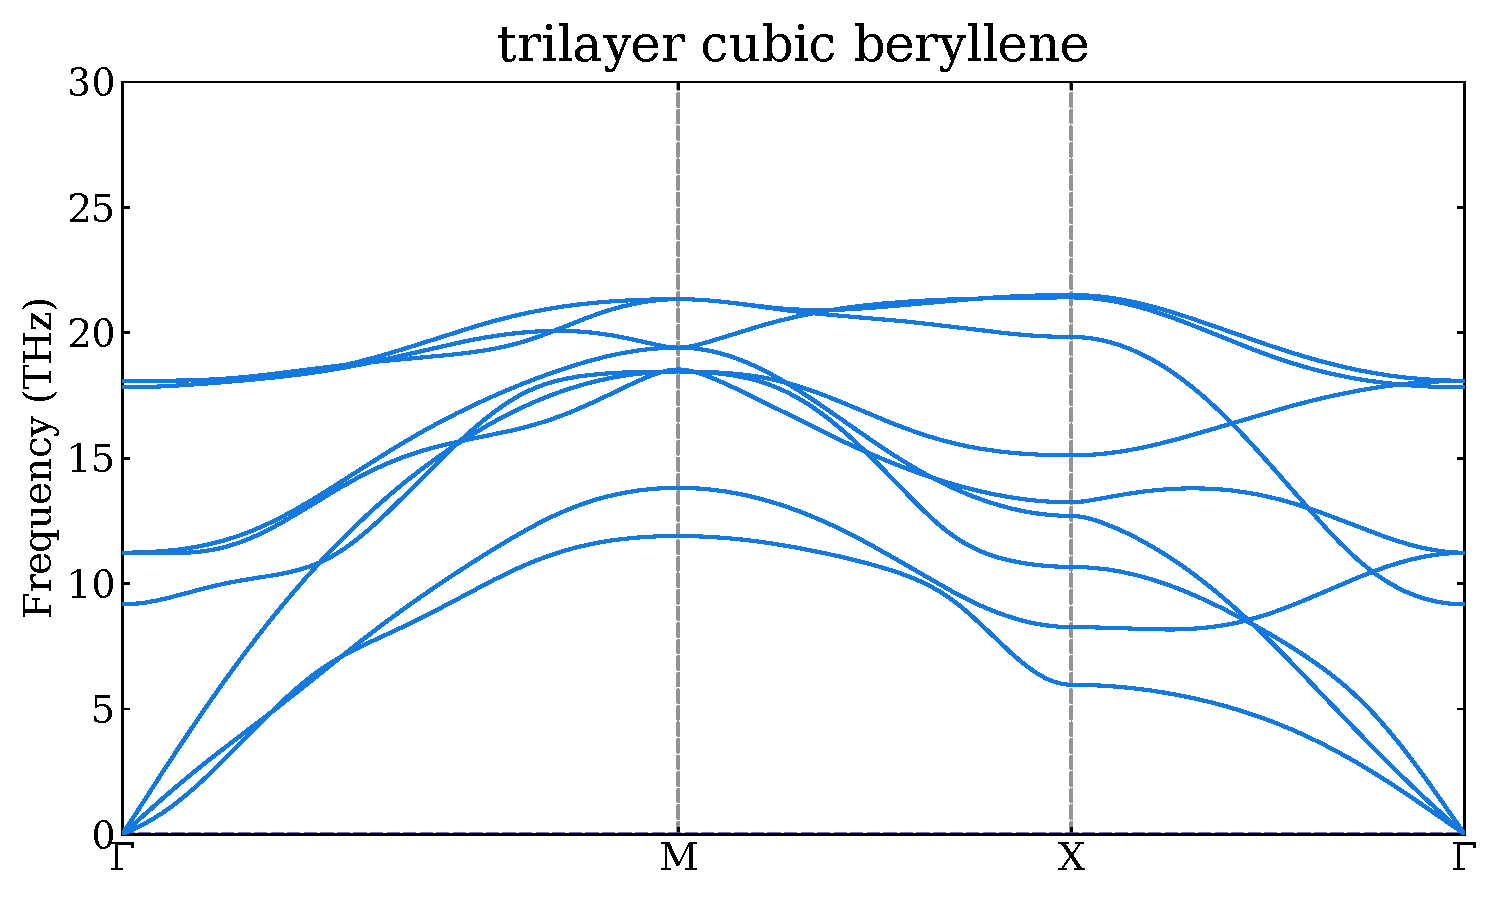
\includegraphics[width=0.40\linewidth]{figures_proj3/phonon_cubic-beryllene-trilayer_thesis.pdf}}%
    &\adjustbox{valign=c}{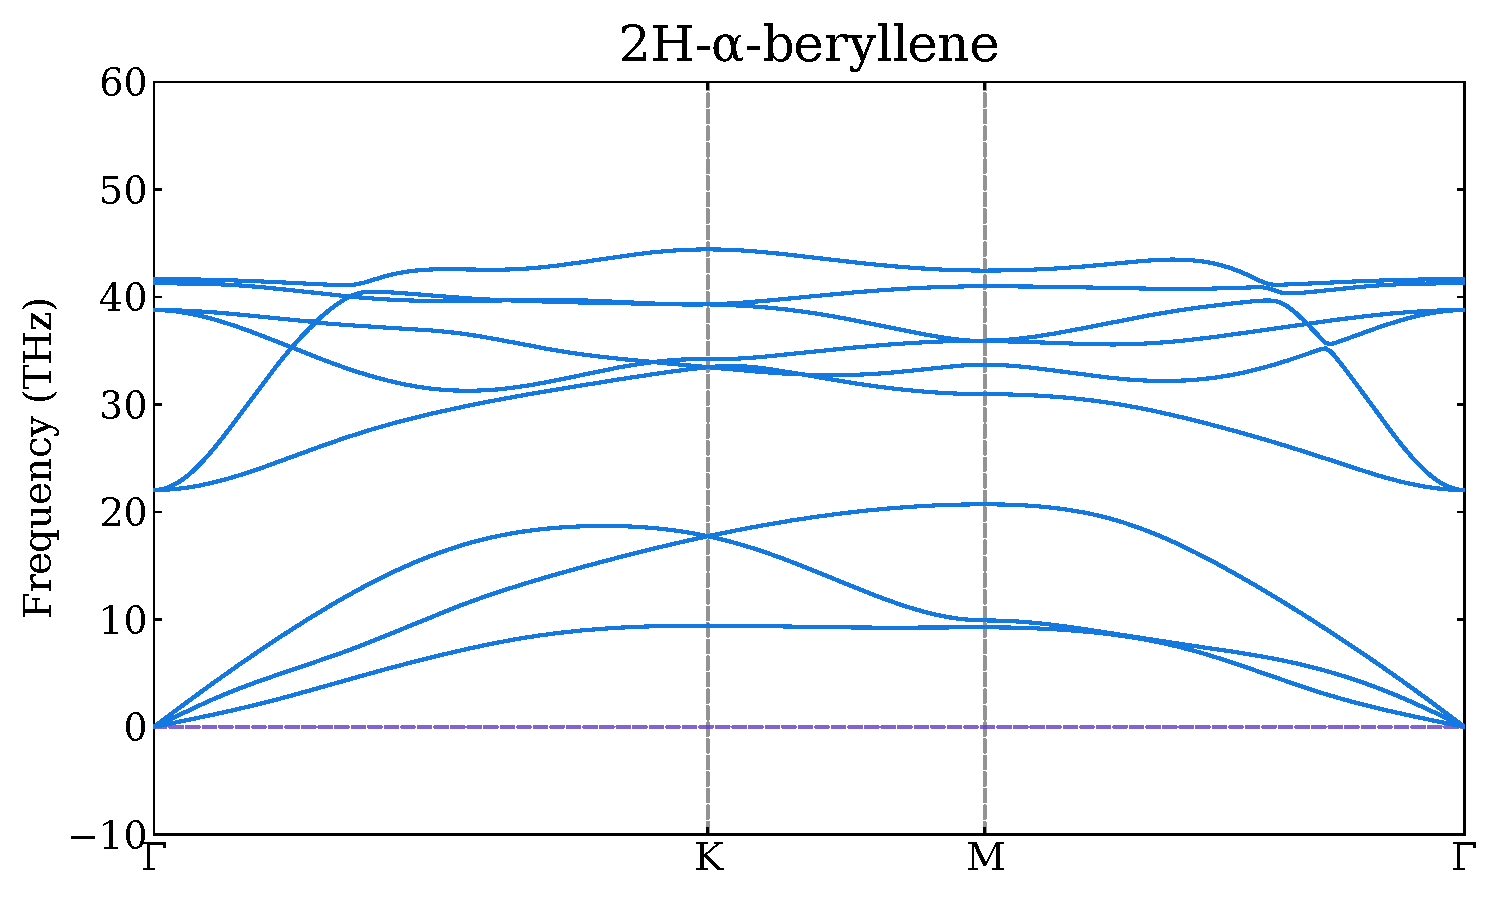
\includegraphics[width=0.40\linewidth]{figures_proj3/phonon_2H-alpha-beryllene_thesis.pdf}}%
    \\\adjustbox{valign=c}{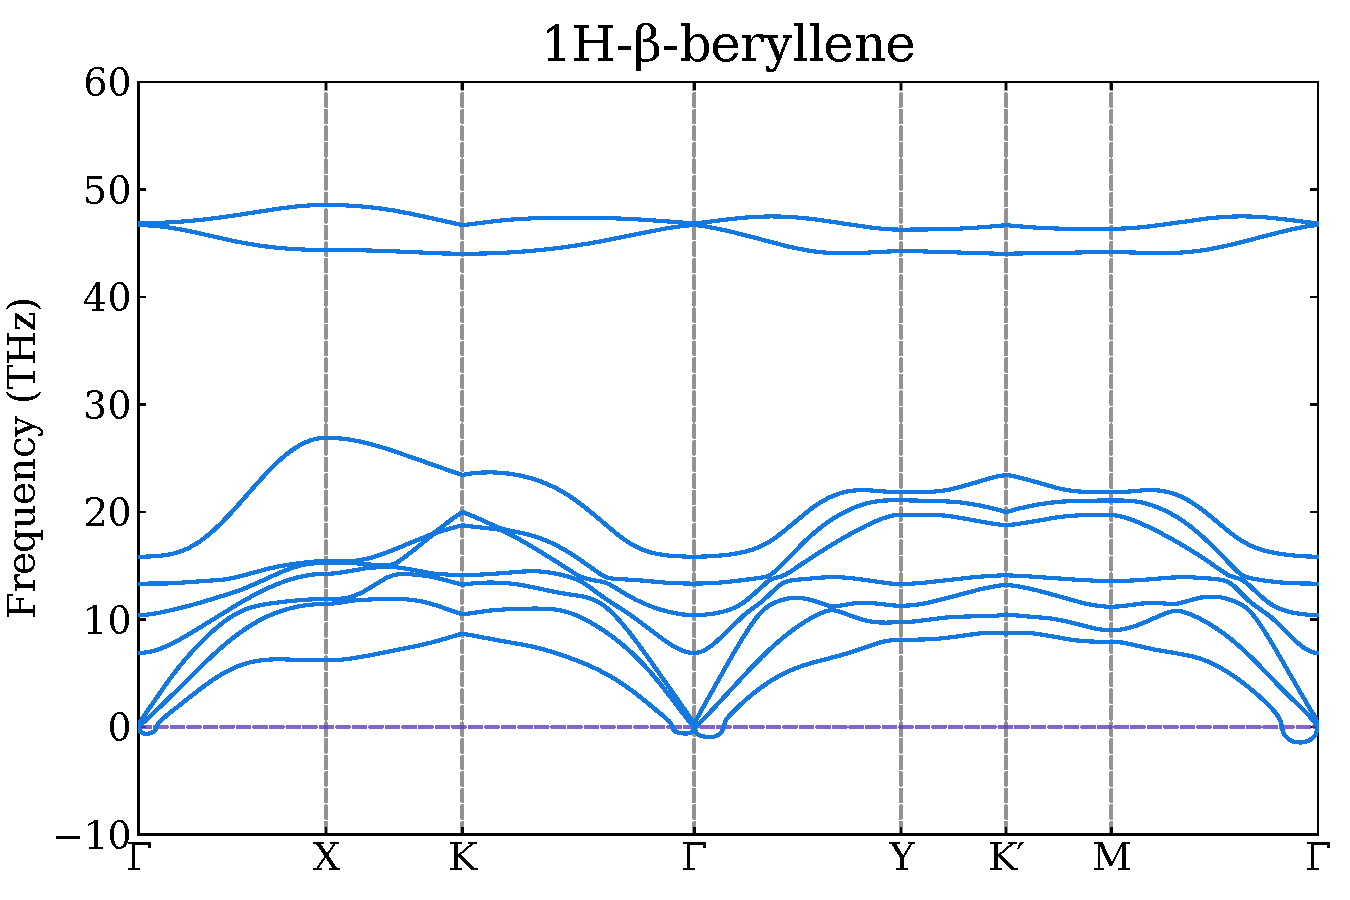
\includegraphics[width=0.40\linewidth]{figures_proj3/phonon_1H-beta-beryllene_thesis.pdf}}%
    &\adjustbox{valign=c}{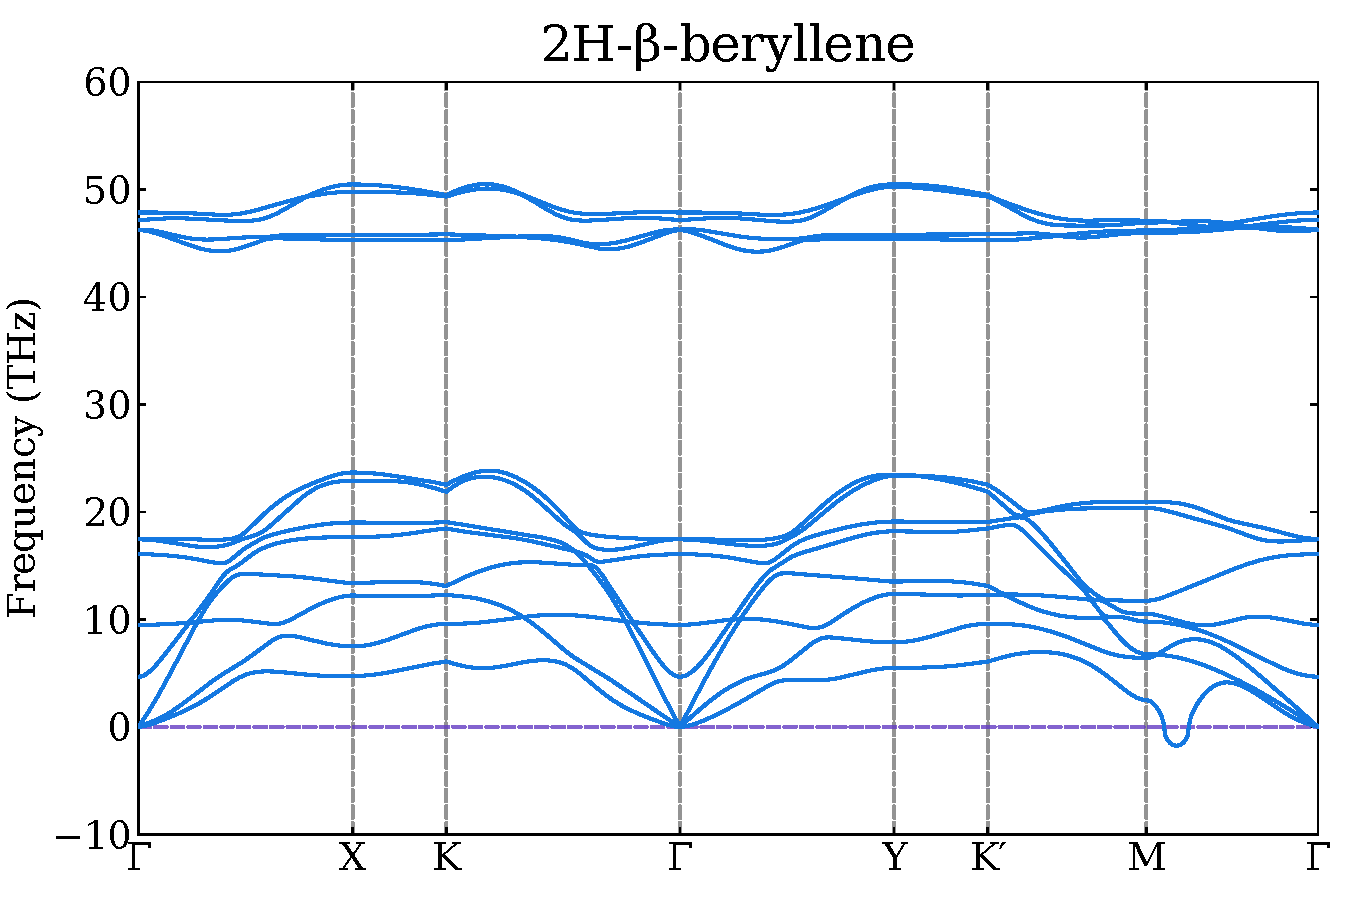
\includegraphics[width=0.40\linewidth]{figures_proj3/phonon_2H-beta-beryllene_thesis.pdf}}%
\end{tabular}
\caption{Phonon dispersion curves of trilayer cubic beryllene and the hydrogen-functionalized beryllene structures.
Upper left: trilayer cubic beryllene; Upper right: 2H-$\alpha$-beryllene;
Lower left: 1H-$\beta$-beryllene; Lower right: 2H-$\beta$-beryllene.
Imaginary frequencies are shown as negative values.}
\label{fig:proj3_cubic_hydrogenated_phonons}
\end{figure}

We further examine the finite-temperature stability of the hydrogen-functionalized structures using \textit{ab initio} molecular dynamics simulations.
The AIMD trajectories and the corresponding atomic structures are shown in figure~\ref{fig:proj3_hydrogenated_aimd}.
For all three hydrogen-functionalized structures,
the total energy fluctuates around a stable average value,
and the temperature fluctuates around the target temperature of \qty{300}{\kelvin}.
The final structures at \qty{5.5}{\pico\second} preserve the beryllene frameworks without structural collapse or hydrogen desorption.
These results support the finite-temperature stability of the hydrogen-functionalized phases.

\begin{figure}[!htbp]
\centering
\begin{tabular}{@{}c@{}c@{}}
    \adjustbox{valign=c}{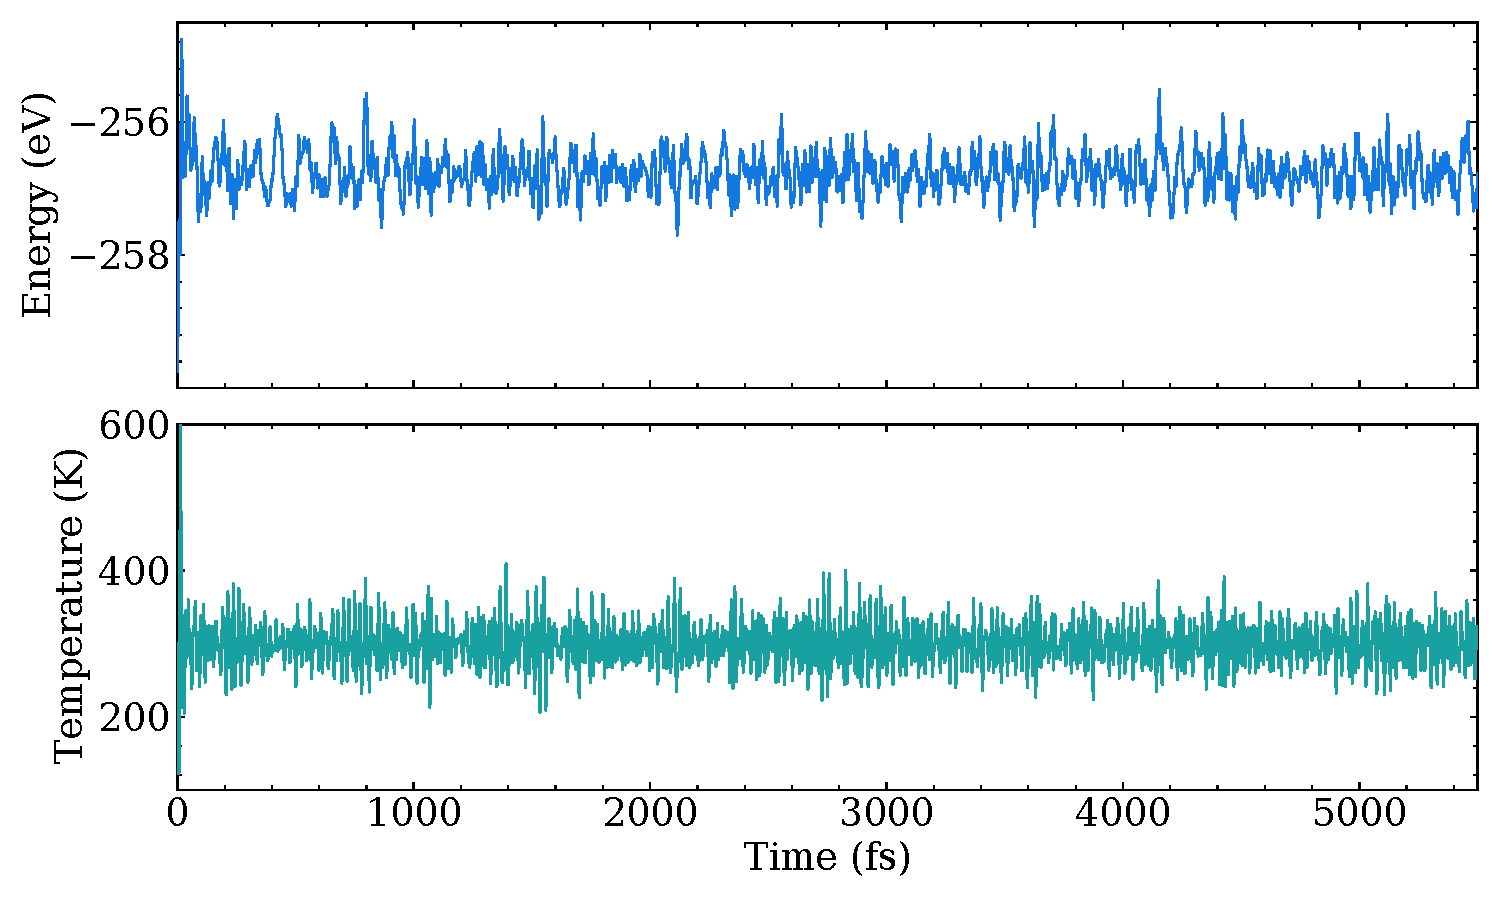
\includegraphics[width=0.50\linewidth]{figures_proj3/aimd_2H-alpha-beryllene_thesis.pdf}}%
    & \adjustbox{valign=c}{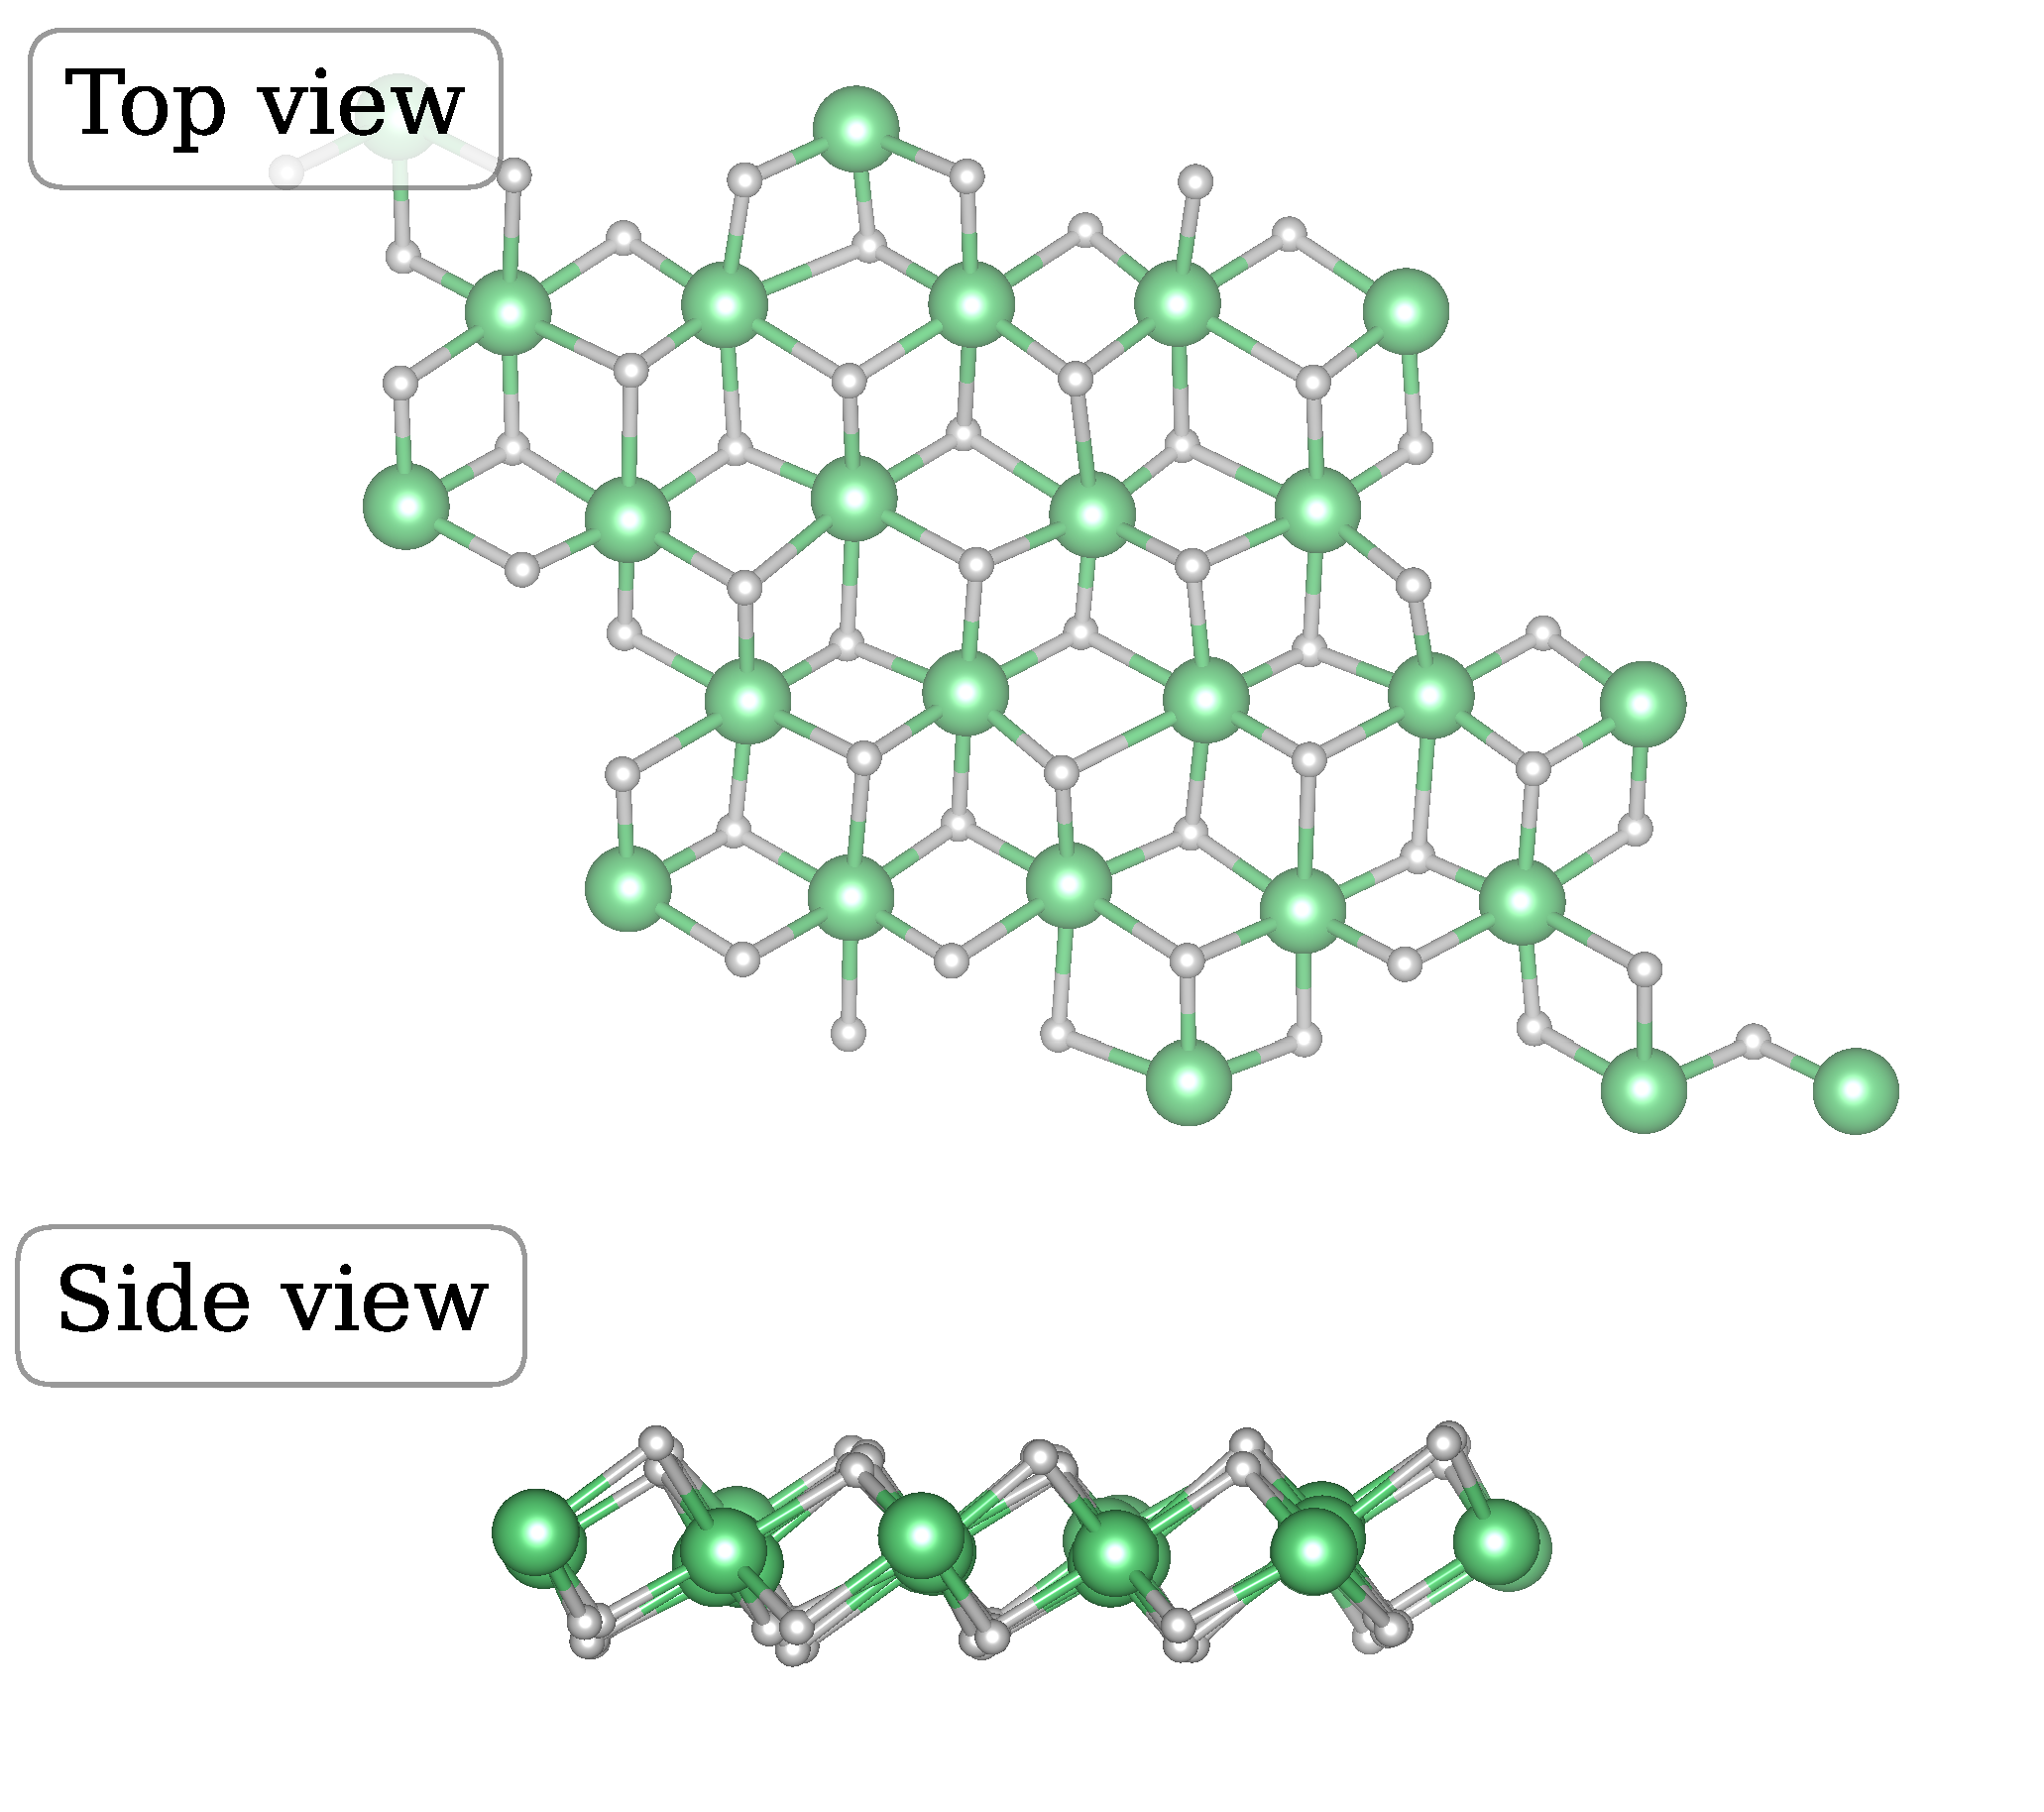
\includegraphics[width=0.30\linewidth]{figures_proj3/structure_2H-alpha-beryllene_thesis.pdf}}\\
    \adjustbox{valign=c}{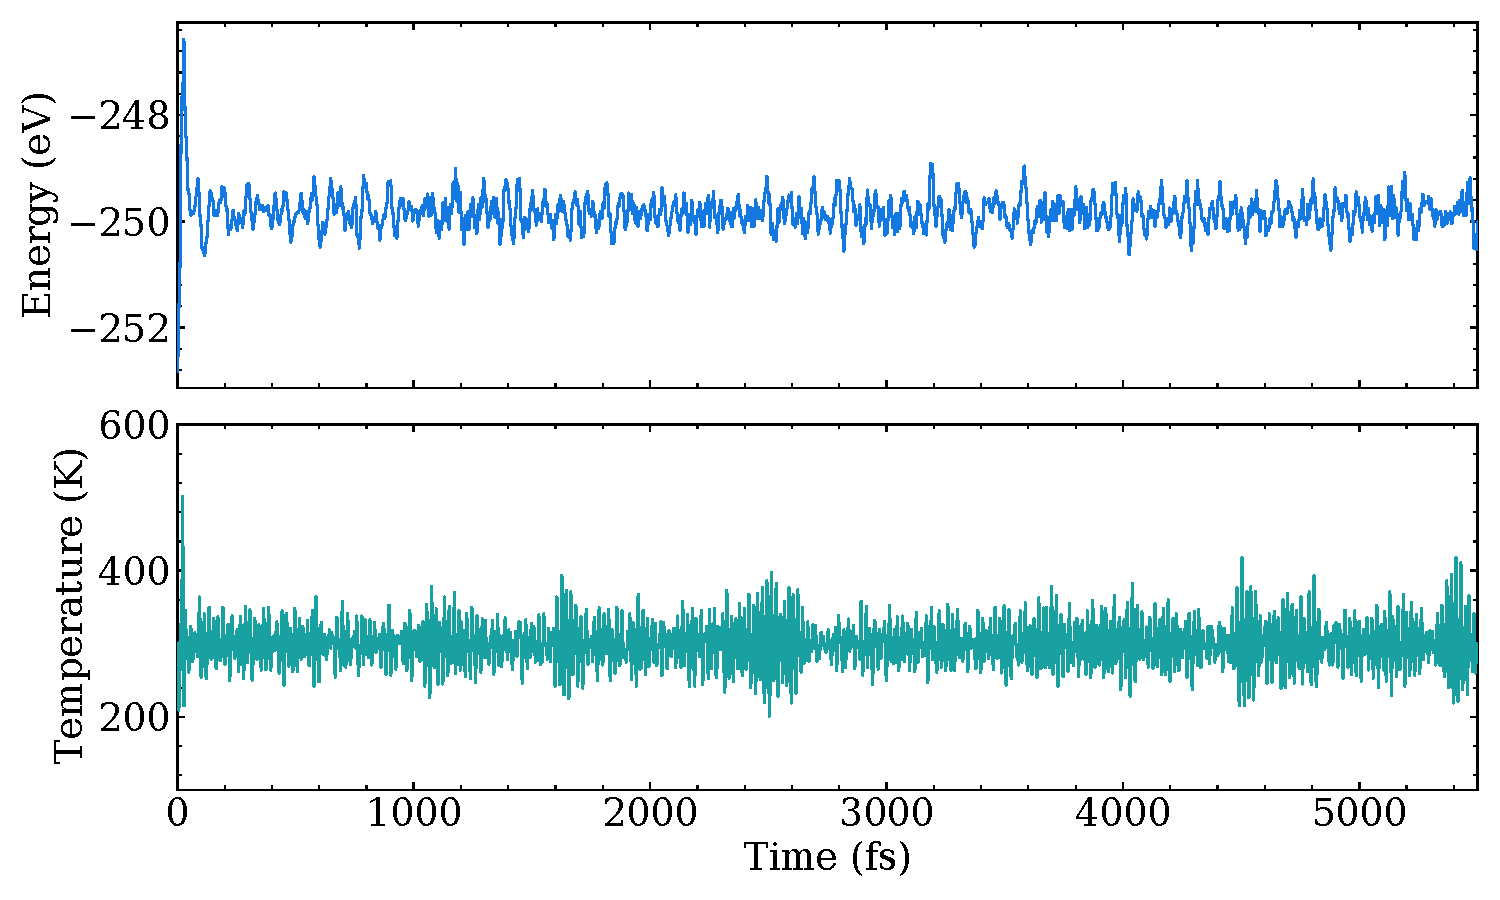
\includegraphics[width=0.50\linewidth]{figures_proj3/aimd_1H-beta-beryllene_thesis.pdf}}%
    & \adjustbox{valign=c}{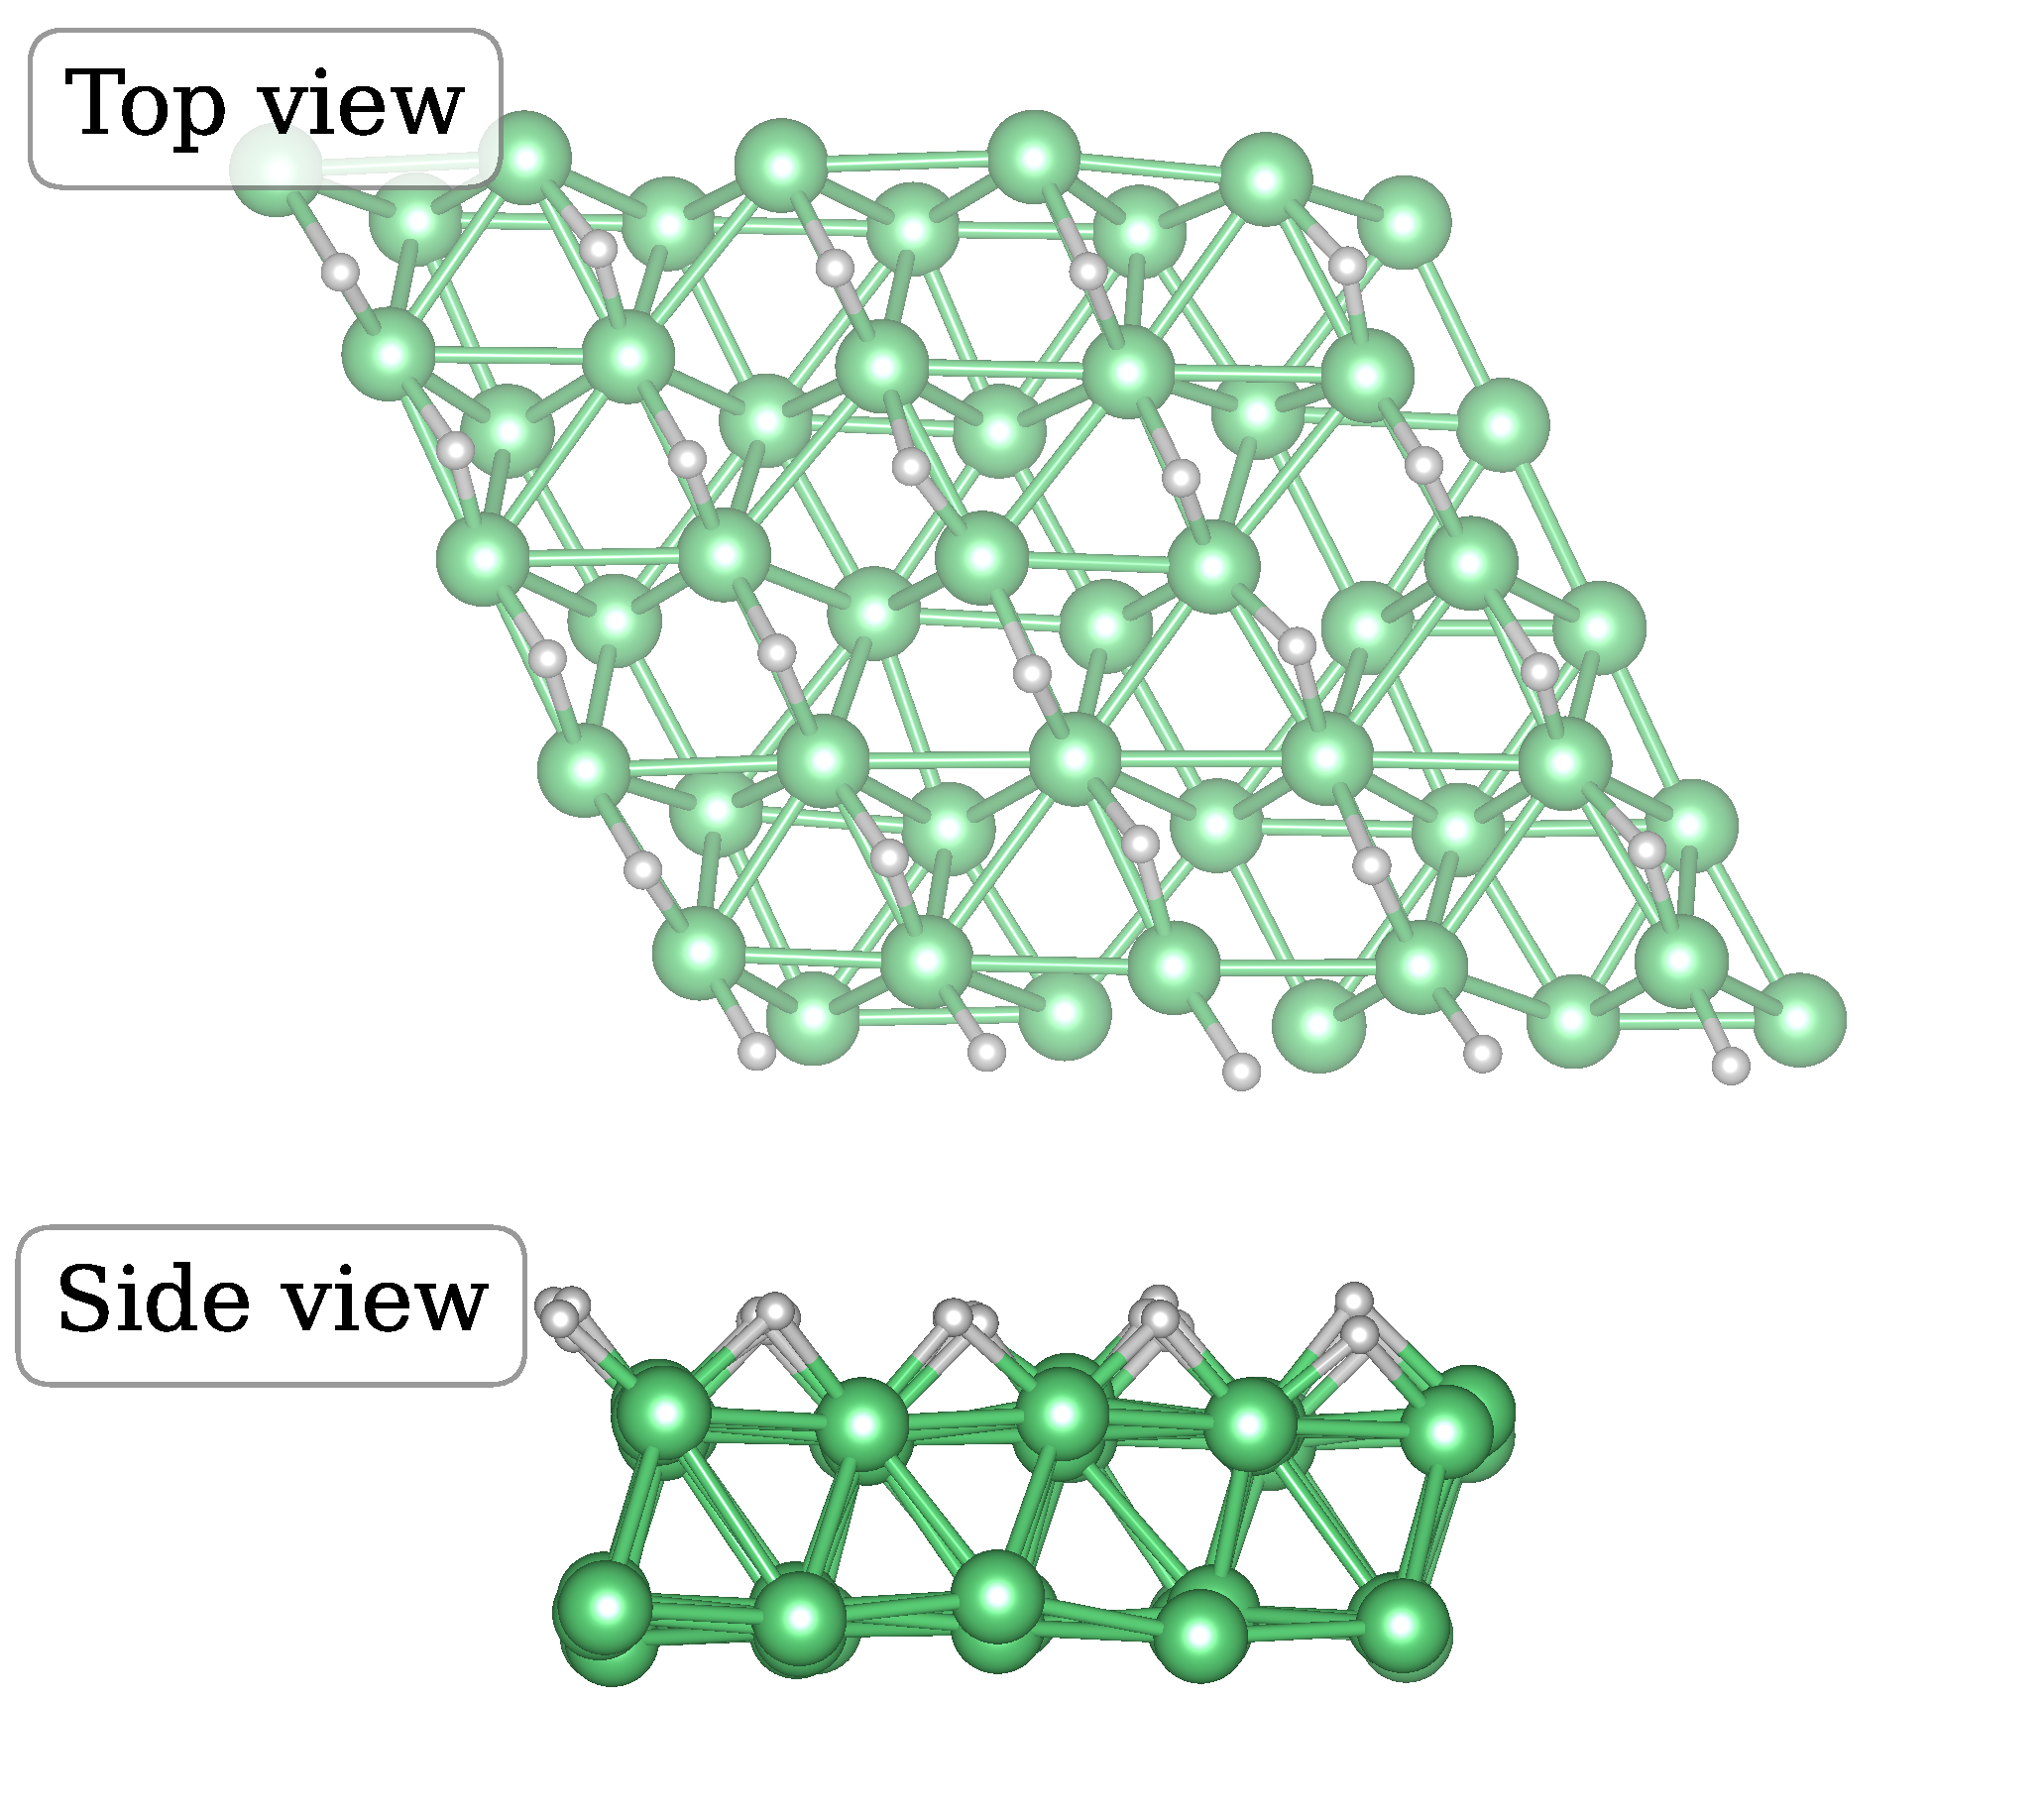
\includegraphics[width=0.30\linewidth]{figures_proj3/structure_1H-beta-beryllene_thesis.pdf}}\\
    \adjustbox{valign=c}{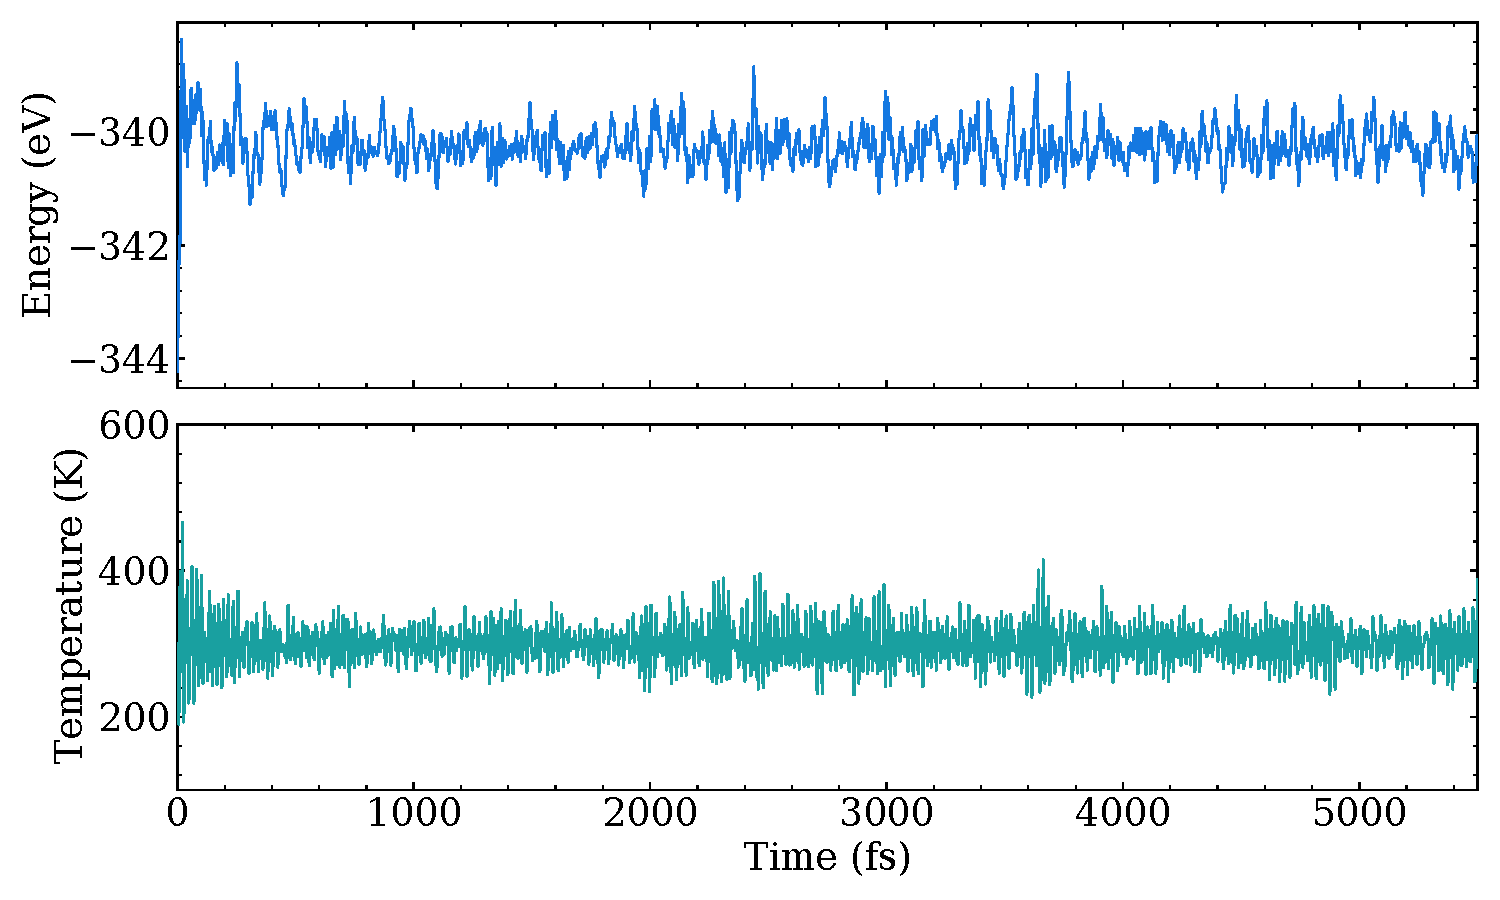
\includegraphics[width=0.50\linewidth]{figures_proj3/aimd_2H-beta-beryllene_thesis.pdf}}%
    & \adjustbox{valign=c}{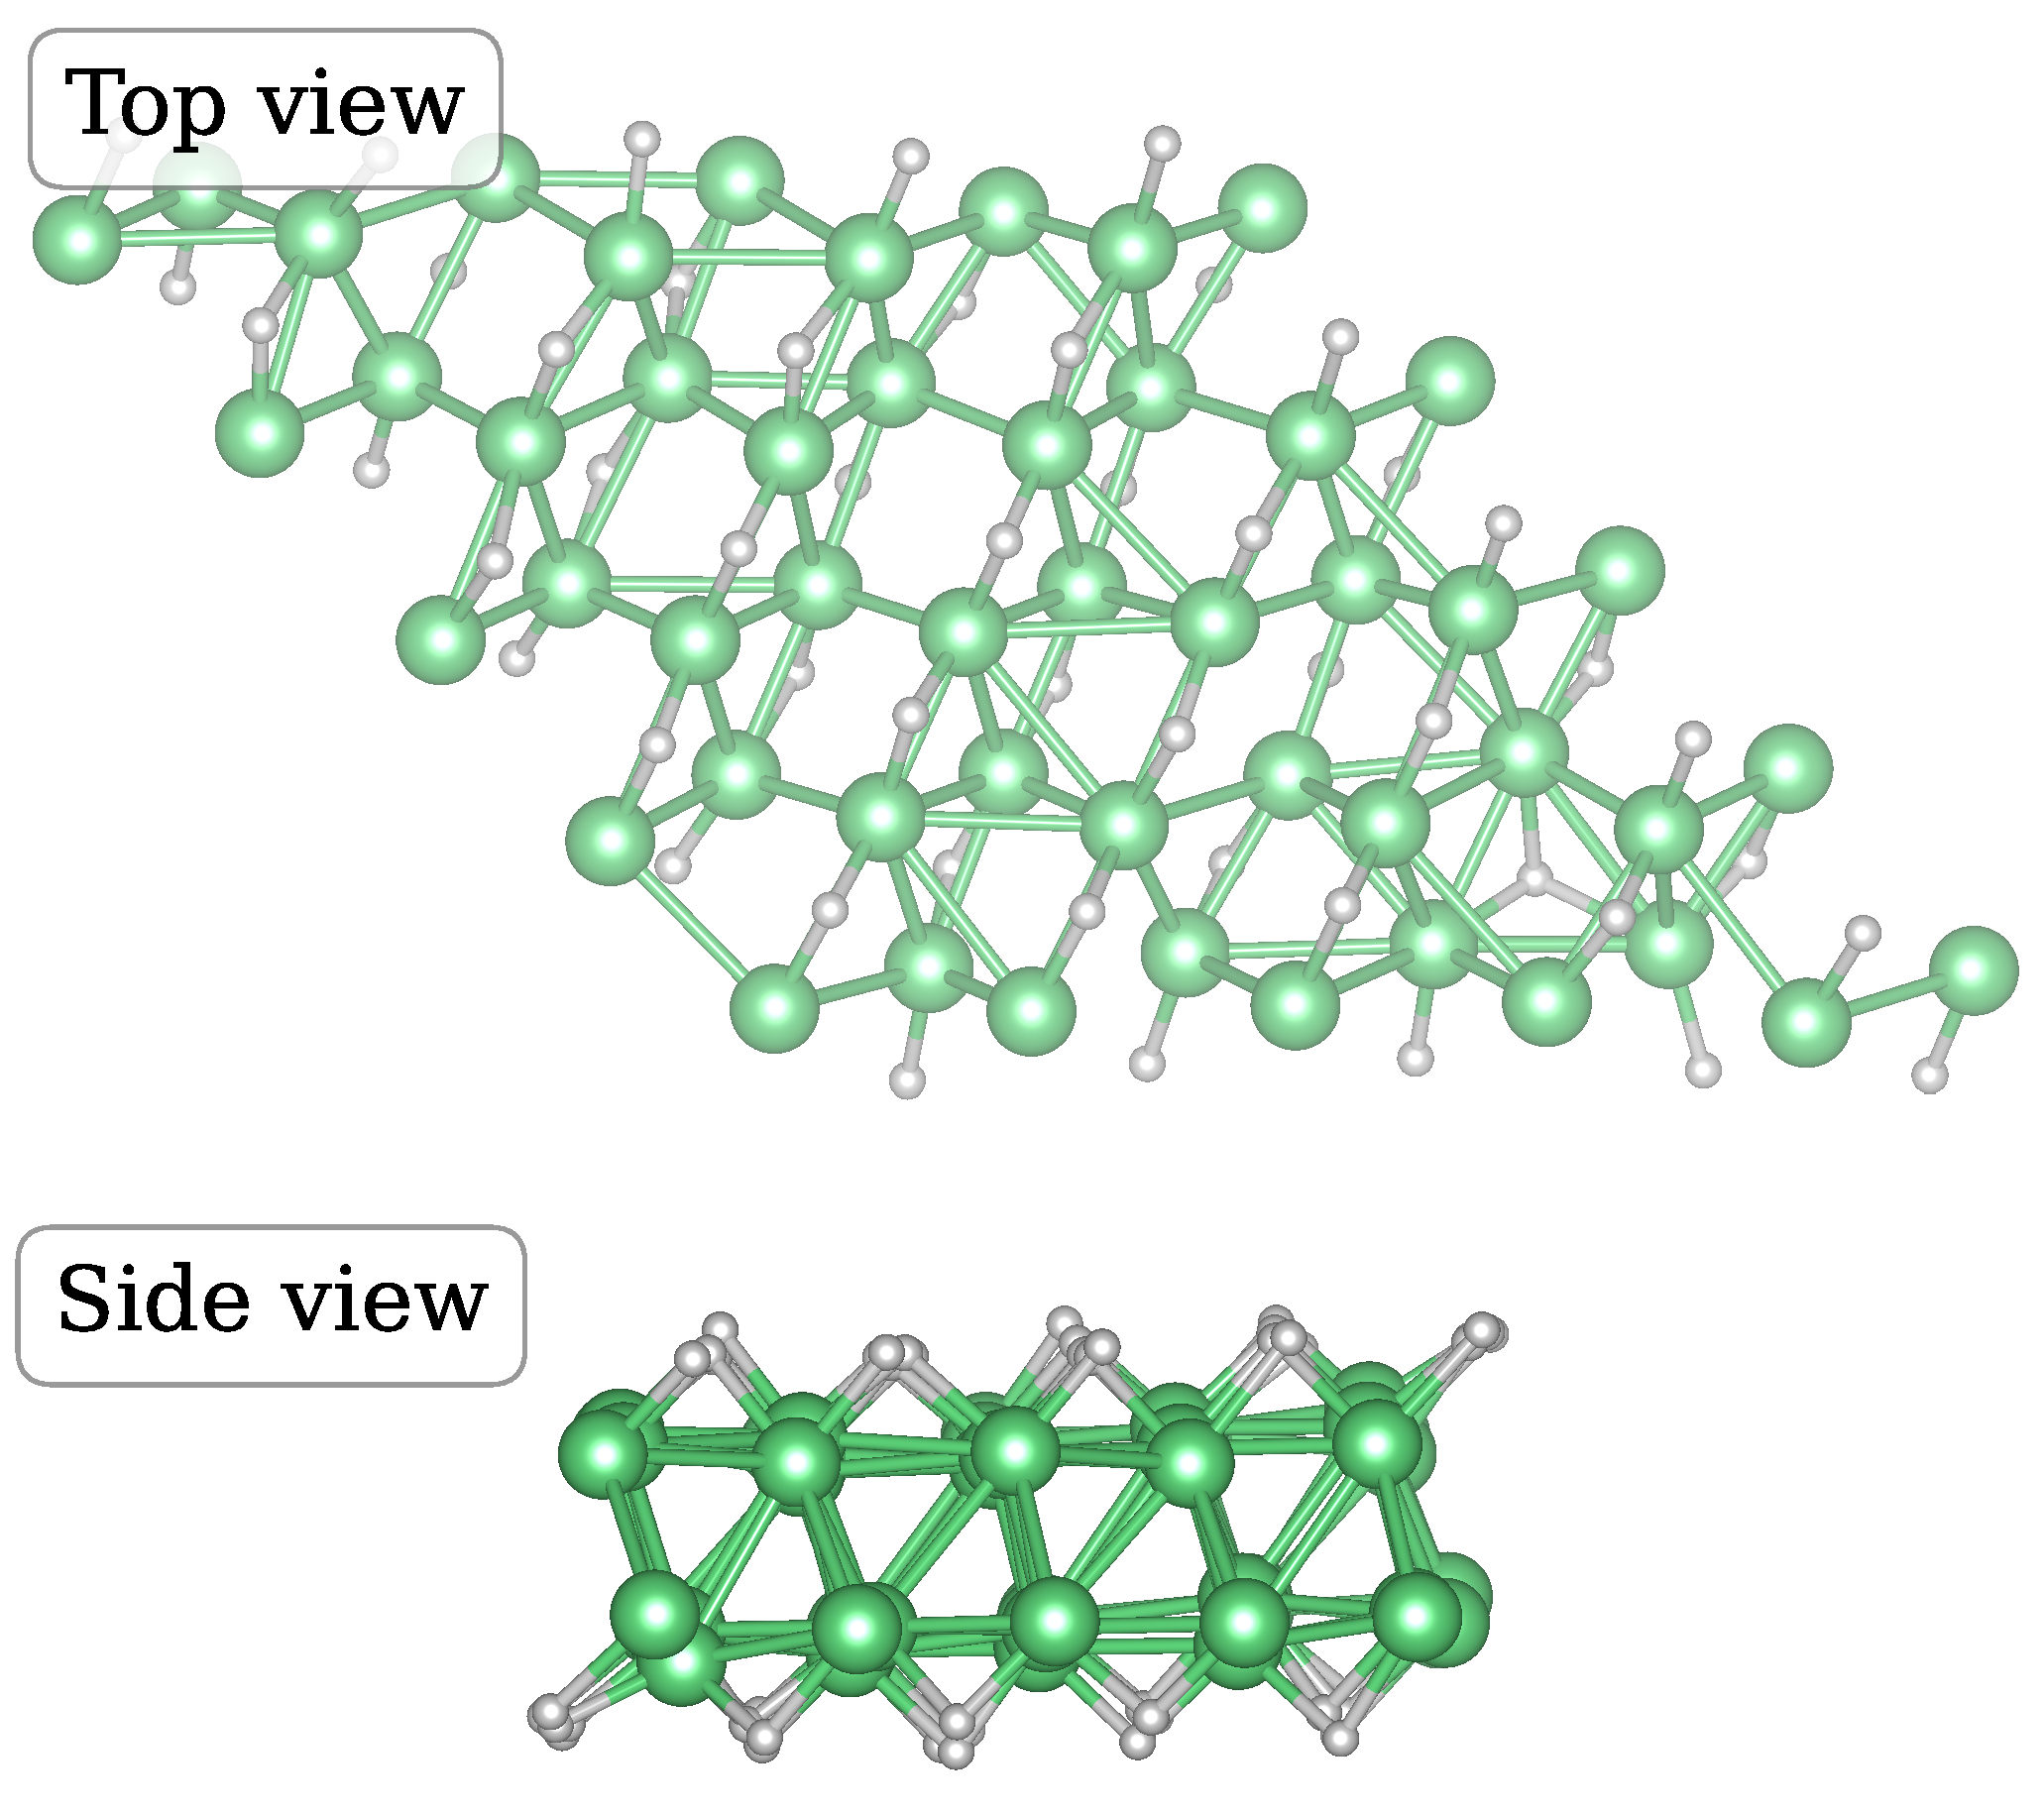
\includegraphics[width=0.30\linewidth]{figures_proj3/structure_2H-beta-beryllene_thesis.pdf}}
\end{tabular}
\caption{\textit{Ab initio} molecular dynamics simulations and corresponding atomic structures of the hydrogen-functionalized beryllene phases.
Upper: 2H-$\alpha$-beryllene;
Middle: 1H-$\beta$-beryllene;
Lower: 2H-$\beta$-beryllene.
For each row,
the left column shows the total energy and temperature as functions of simulation time,
and the right column shows the top and side views of the final structure at \qty{5.5}{\pico\second},
with beryllium in green and hydrogen in grey.}
\label{fig:proj3_hydrogenated_aimd}
\end{figure}

\subsection{Hydrogen adsorption energetics}
\label{3_hydrogen_adsorption_energetics}

The optimized structural parameters of the hydrogen-functionalized structures are listed in table~\ref{tab:proj3_hydrogenated_structural_parameters}.
For 2H-$\alpha$-beryllene,
the in-plane lattice constant increases from \qty{2.129}{\angstrom} in pristine $\alpha$-beryllene to \qty{2.322}{\angstrom} after hydrogen adsorption.
For 1H-$\beta$-beryllene,
hydrogen adsorption breaks the hexagonal symmetry:
the two in-plane lattice constants become \qty{2.322}{\angstrom} and \qty{2.108}{\angstrom},
with an angle of \qty{117}{\degree} between the lattice vectors.
For 2H-$\beta$-beryllene,
the two lattice vectors have the same magnitude of \qty{2.596}{\angstrom},
with an angle of \qty{133}{\degree}.
This geometry forms a rhombic lattice.
The hydrogen adsorption energies relative to \ce{H2} are \qty{-0.33}{\electronvolt},
\qty{-0.07}{\electronvolt},
and \qty{-0.17}{\electronvolt} per hydrogen atom for 2H-$\alpha$-beryllene,
1H-$\beta$-beryllene,
and 2H-$\beta$-beryllene,
respectively.
These negative adsorption energies indicate that hydrogen adsorption is exothermic for all three structures,
although only weakly for the $\beta$-based structures.

The zero-point energies of the beryllene layers and of the \ce{H2} molecule raise these values to \qty{-0.24}{\electronvolt},
\qty{0.01}{\electronvolt},
and \qty{-0.09}{\electronvolt} per hydrogen atom,
respectively.
At \qty{298}{\kelvin} and \qty{1}{\bar} of \ce{H2},
the corresponding adsorption free energies are \qty{-0.08}{\electronvolt},
\qty{0.17}{\electronvolt},
and \qty{0.06}{\electronvolt} per hydrogen atom.
Therefore,
only 2H-$\alpha$-beryllene is thermodynamically stable against \ce{H2} release under ambient conditions.
2H-$\beta$-beryllene requires an equilibrium \ce{H2} pressure of approximately \qty{90}{\bar} at room temperature,
whereas 1H-$\beta$-beryllene can exist only as a kinetically trapped phase.
These energetics are summarized in table~\ref{tab:proj3_hydrogenation_energetics} in section~\ref{3_supplementary}.

2H-$\alpha$-beryllene has the composition of \ce{BeH2}.
We therefore also compare it with two square \ce{BeH2} monolayers relaxed with the same settings.
A puckered square layer,
in which each beryllium atom is tetrahedrally coordinated by four bridging hydrogen atoms at \qty{1.468}{\angstrom},
as in bulk \ce{BeH2},
is \qty{38}{\milli\electronvolt} per formula unit lower in energy than 2H-$\alpha$-beryllene,
whereas a planar square layer is \qty{1.23}{\electronvolt} per formula unit higher.
2H-$\alpha$-beryllene is therefore metastable with respect to the puckered square layer.
Since this transformation requires the triangular beryllium lattice to rearrange into a square lattice,
2H-$\alpha$-beryllene can remain kinetically stable as the product of hydrogenating $\alpha$-beryllene.
Only these two square configurations are considered,
so this comparison does not replace a global structure search~\cite{li2018global}.
The polymorph energies are listed in table~\ref{tab:proj3_beh2_polymorphs}.

\begin{table}[!htbp]
\centering
\rowcolors{2}{gray!15}{white}
\begin{adjustbox}{center,max width=1.0\linewidth}
\begin{tabular}{cccccccc}
\hline
\rowcolor{gray!25}
system
& $a$
& $b$
& interlayer Be-Be (\AA)
& H-Be (\AA)
& $E_{\mathrm{ad}}$ (eV)
& angle
& electronic nature \\
\hline
2H-$\alpha$-beryllene
& 2.322 & 2.322 & -- & 1.599 & $-0.33$ & $120^{\circ}$ & semiconductor \\
1H-$\beta$-beryllene
& 2.322 & 2.108 & 1.849 & 1.451 & $-0.07$ & $117^{\circ}$ & metallic \\
2H-$\beta$-beryllene
& 2.596 & 2.596 & 1.786 & 1.446 & $-0.17$ & $133^{\circ}$ & metallic \\
\hline
\end{tabular}
\end{adjustbox}
\caption{Lattice vectors $a$ and $b$,
interlayer Be-Be distance, H-Be bond length,
hydrogen adsorption energy $E_{\mathrm{ad}}$ per hydrogen atom relative to \ce{H2},
angle between the two in-plane lattice vectors,
and electronic nature of the hydrogen-functionalized beryllene structures.
The lattice vectors, interlayer Be-Be distance,
and H-Be bond length are given in \si{\angstrom},
while the adsorption energy is given in \si{\electronvolt}.}
\label{tab:proj3_hydrogenated_structural_parameters}
\end{table}

\subsection{Electronic properties}
\label{3_electronic_properties}

We now examine the electronic properties of pristine and hydrogen-functionalized beryllene structures.
The band structures of pristine $\alpha$-beryllene and $\beta$-beryllene are shown in figure~\ref{fig:proj3_band_structures} in section~\ref{3_supplementary},
and agree well with previous calculations~\cite{li2023coexistence}.
The band structures of trilayer cubic beryllene and the hydrogen-functionalized structures are shown in figure~\ref{fig:proj3_band_structures_cubic_hydrogenated}.

The trilayer cubic beryllene structure shows metallic behaviour,
with multiple bands crossing the Fermi level.
The bands near the Fermi level show moderate dispersion,
which suggests delocalized electronic states and good in-plane conductivity.
Around the $\Gamma$,
$\mathrm{M}$,
and $\mathrm{X}$ points,
noticeable band splitting appears,
consistent with interlayer coupling in the trilayer structure.
The coexistence of relatively flat bands and dispersive unoccupied bands at higher energies further indicates a mixture of localized and itinerant electronic states.

Hydrogen functionalization changes the electronic structure differently for the $\alpha$ and $\beta$ phases.
For 2H-$\alpha$-beryllene,
the band structure shows a wide indirect band gap of \qty{4.84}{\electronvolt} at the PBE level.
Since PBE generally underestimates band gaps,
we also calculate the band structure of this structure with the HSE06 hybrid functional.
HSE06 increases the indirect band gap to \qty{6.00}{\electronvolt},
while the valence-band maximum and the conduction-band minimum remain at the same wave vectors.
In contrast,
both 1H-$\beta$-beryllene and 2H-$\beta$-beryllene remain metallic,
with bands crossing the Fermi level.
These results show that hydrogen functionalization opens a large gap in $\alpha$-beryllene,
whereas the hydrogen-functionalized $\beta$-based structures preserve their metallic character.

\begin{figure}[!htbp]
\centering
\begin{tabular}{@{}cc@{}}
    \adjustbox{valign=c}{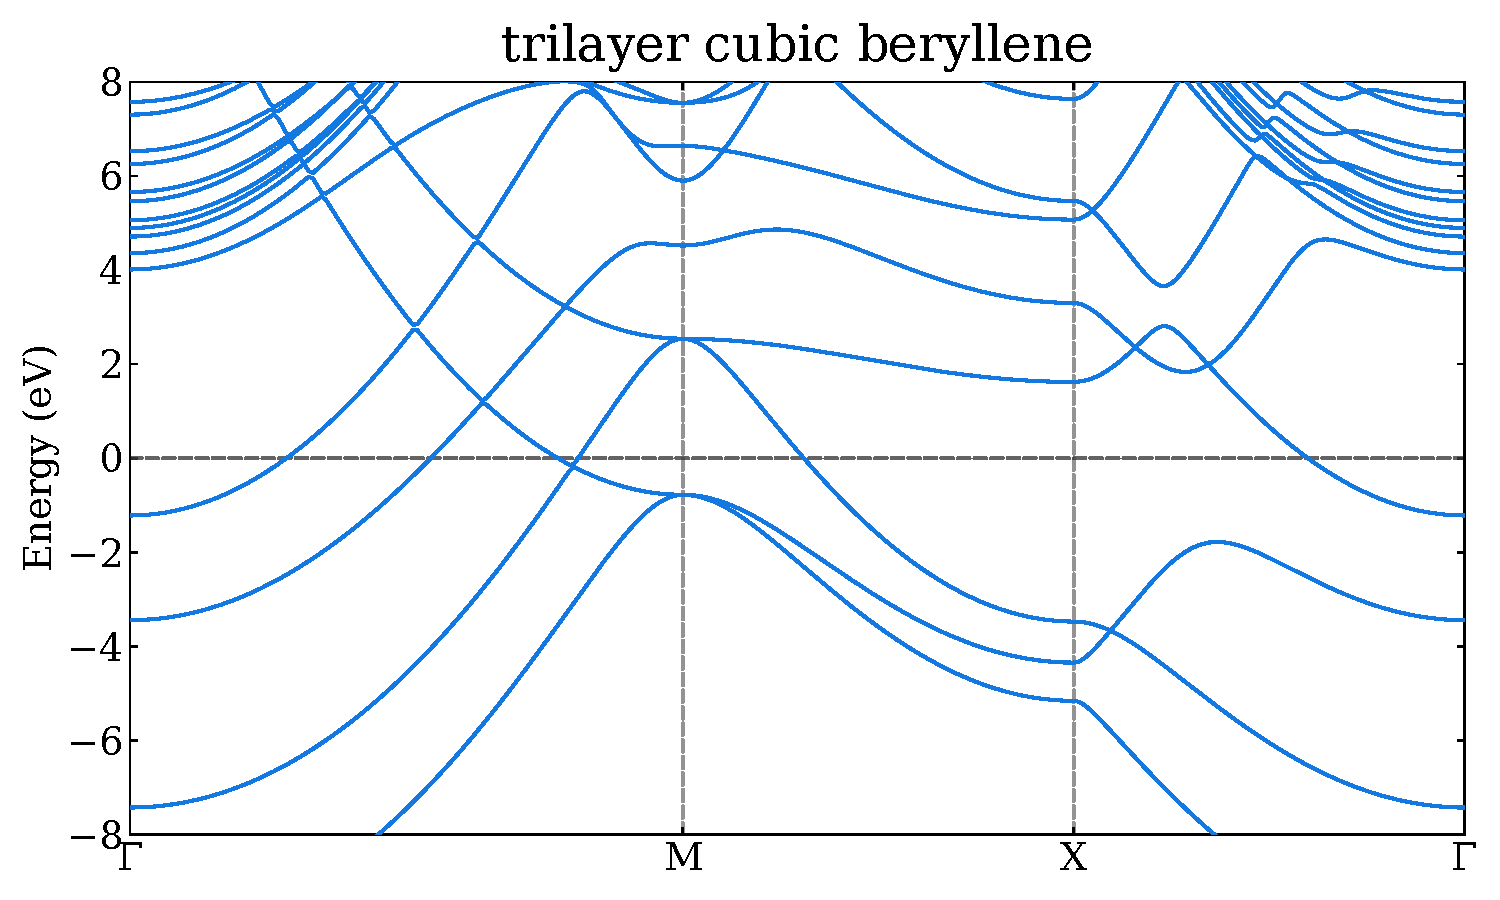
\includegraphics[width=0.40\linewidth]{figures_proj3/bands_cubic-beryllene-trilayer_thesis.pdf}}&
    \adjustbox{valign=c}{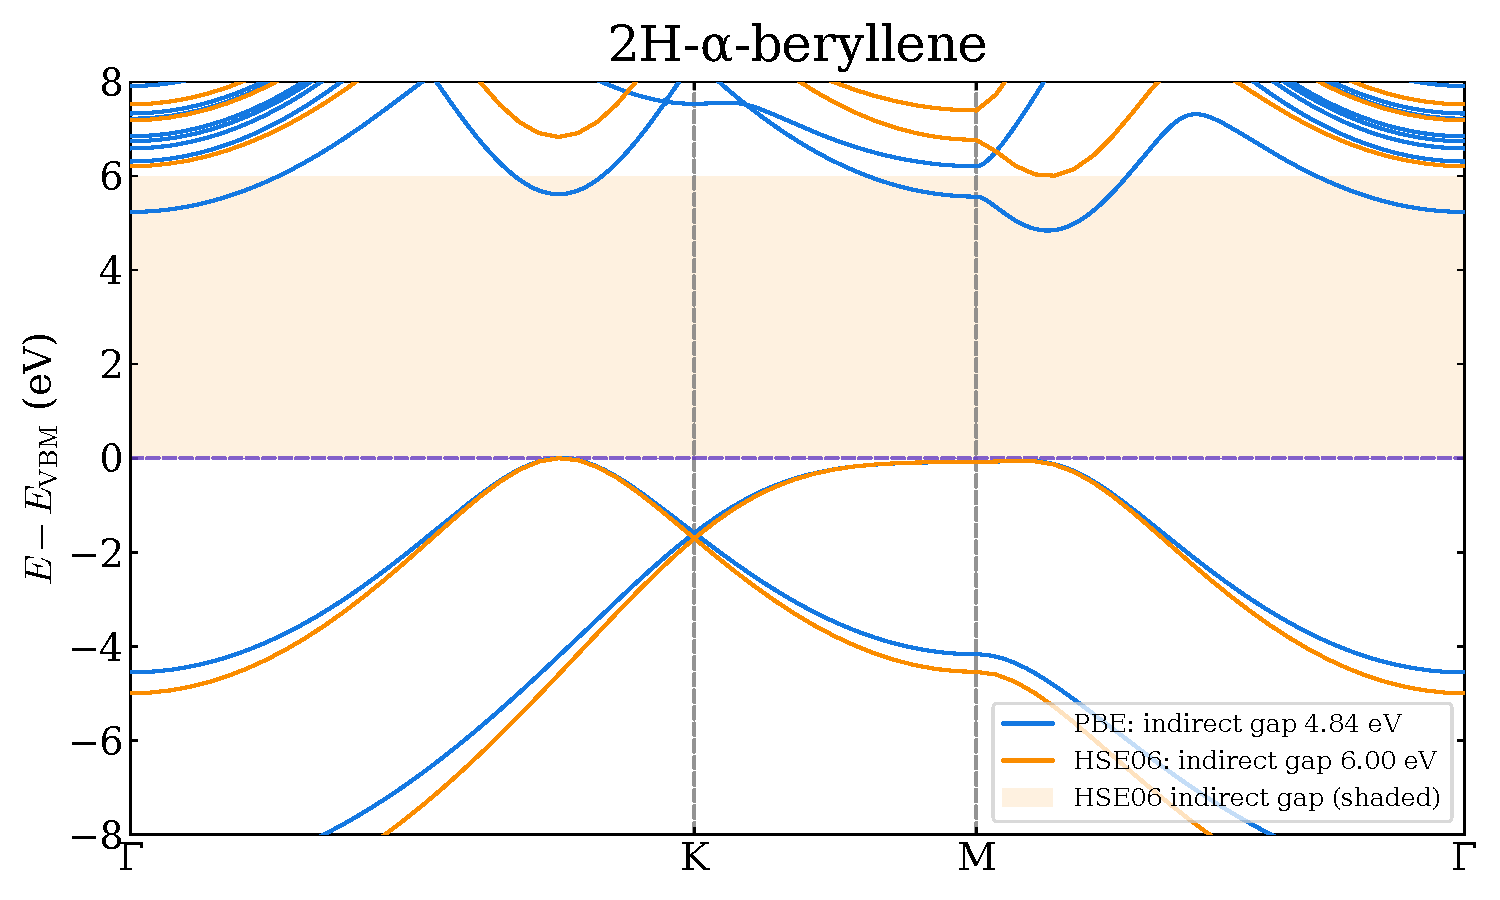
\includegraphics[width=0.40\linewidth]{figures_proj3/bands_2H-alpha-beryllene_thesis.pdf}}\\
    \adjustbox{valign=c}{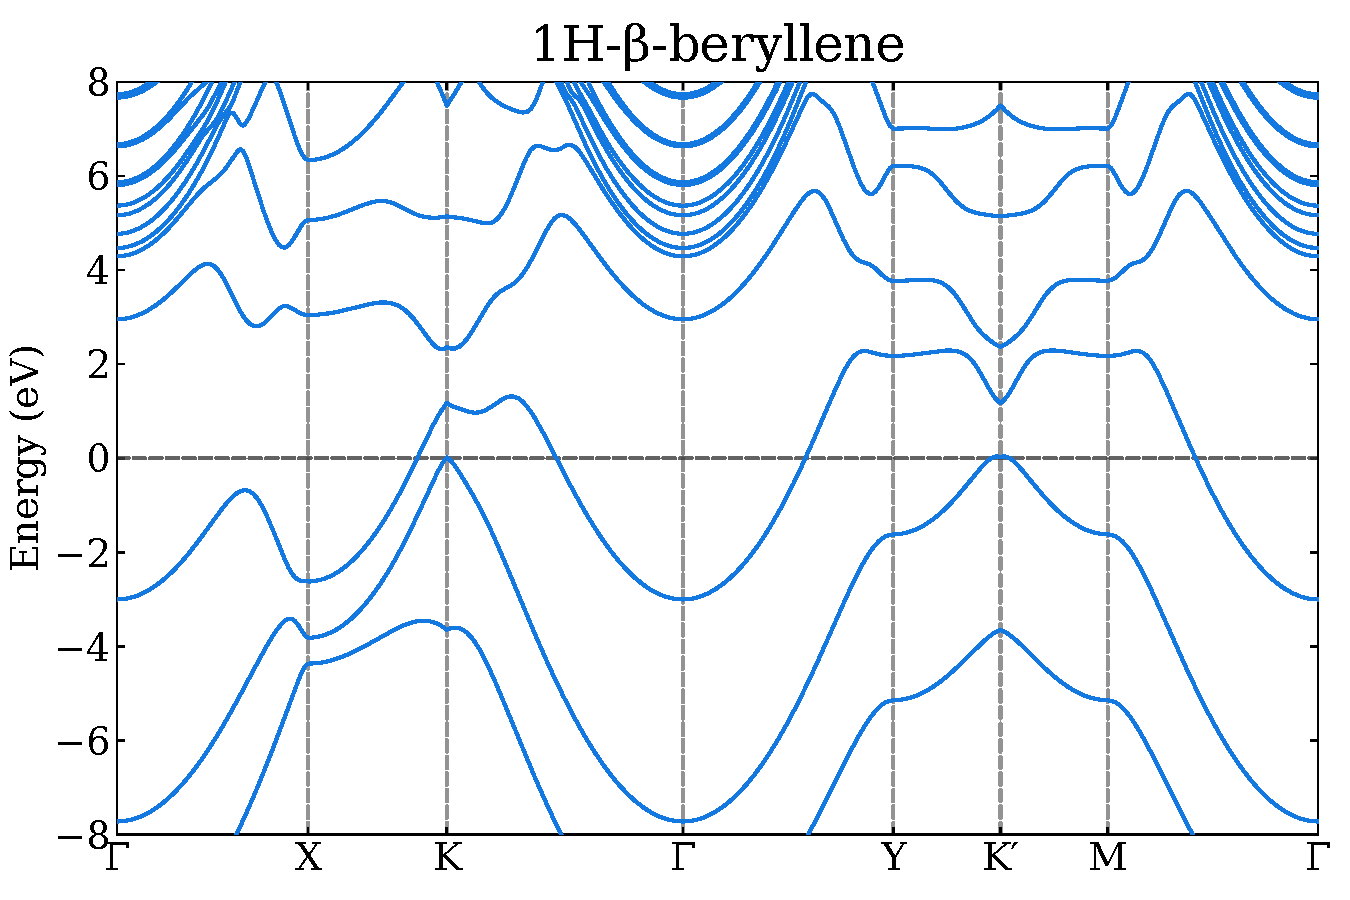
\includegraphics[width=0.40\linewidth]{figures_proj3/bands_1H-beta-beryllene_thesis.pdf}}&
    \adjustbox{valign=c}{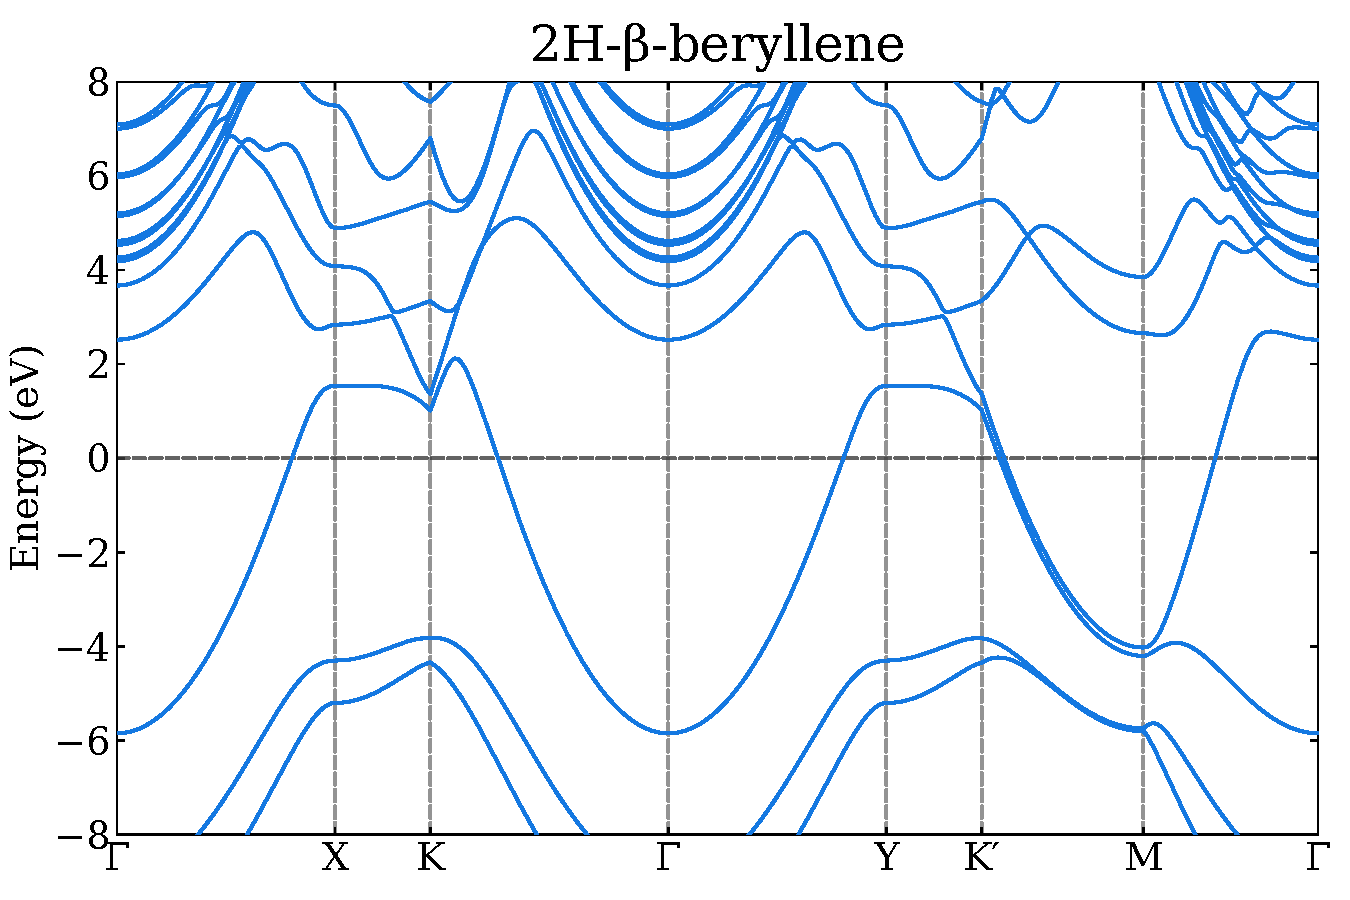
\includegraphics[width=0.40\linewidth]{figures_proj3/bands_2H-beta-beryllene_thesis.pdf}}
\end{tabular}
\caption{Band structures of trilayer cubic beryllene and the hydrogen-functionalized beryllene structures.
Upper left: trilayer cubic beryllene; Upper right: 2H-$\alpha$-beryllene;
Lower left: 1H-$\beta$-beryllene; Lower right: 2H-$\beta$-beryllene.
For 1H-$\beta$-beryllene and 2H-$\beta$-beryllene,
the path $\Gamma$--$\mathrm{X}$--$\mathrm{K}$--$\Gamma$--$\mathrm{Y}$--$\mathrm{K}'$--$\mathrm{M}$--$\Gamma$ passes through all four time-reversal invariant momenta and the zone corners $\mathrm{K}$ and $\mathrm{K}'$,
as for the phonon dispersions in figure~\ref{fig:proj3_cubic_hydrogenated_phonons}.
For 2H-$\alpha$-beryllene,
the PBE (blue) and HSE06 (orange) bands are each aligned at their valence-band maximum.}
\label{fig:proj3_band_structures_cubic_hydrogenated}
\end{figure}

The density of states further supports the band-structure interpretation.
Figure~\ref{fig:proj3_dos_cubic_trilayer} compares the total density of states of bulk bcc beryllium and trilayer cubic beryllene.
Trilayer cubic beryllene has a finite density of states at the Fermi level,
consistent with its metallic band structure.

\begin{figure}[!htbp]
\centering
    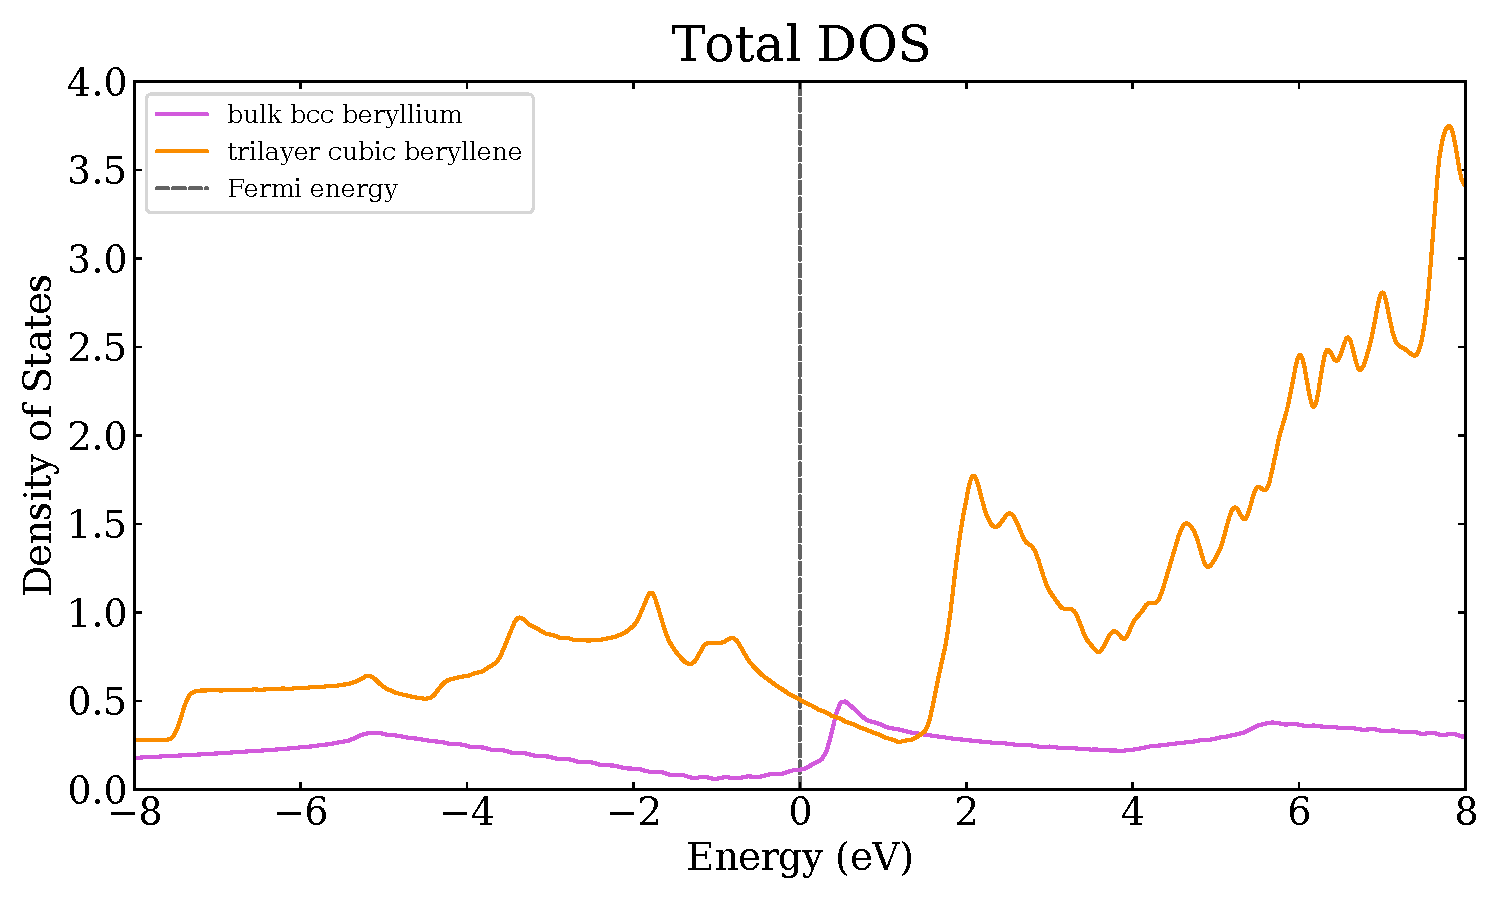
\includegraphics[width=0.6\linewidth]{figures_proj3/dos_cubic-family_thesis.pdf}
\caption{Total density of states of bulk bcc beryllium and trilayer cubic beryllene.}
\label{fig:proj3_dos_cubic_trilayer}
\end{figure}

The total and projected densities of states of pristine and hydrogen-functionalized beryllene structures are shown in figure~\ref{fig:proj3_dos_hydrogenated}.
For 2H-$\alpha$-beryllene,
the density of states vanishes around the Fermi level,
consistent with the wide-gap semiconducting band structure.
For 1H-$\beta$-beryllene and 2H-$\beta$-beryllene,
the finite density of states at the Fermi level confirms their metallic behaviour.
The projected densities of states show strong hybridization among beryllium $s$ and $p$ states,
together with the hydrogen $1s$ state in the hydrogen-functionalized structures.
This hybridization reflects the modification of the local bonding environment after hydrogen functionalization.

\begin{figure}[!htbp]
\centering
\begin{tabular}{@{}cc@{}}
    \adjustbox{valign=c}{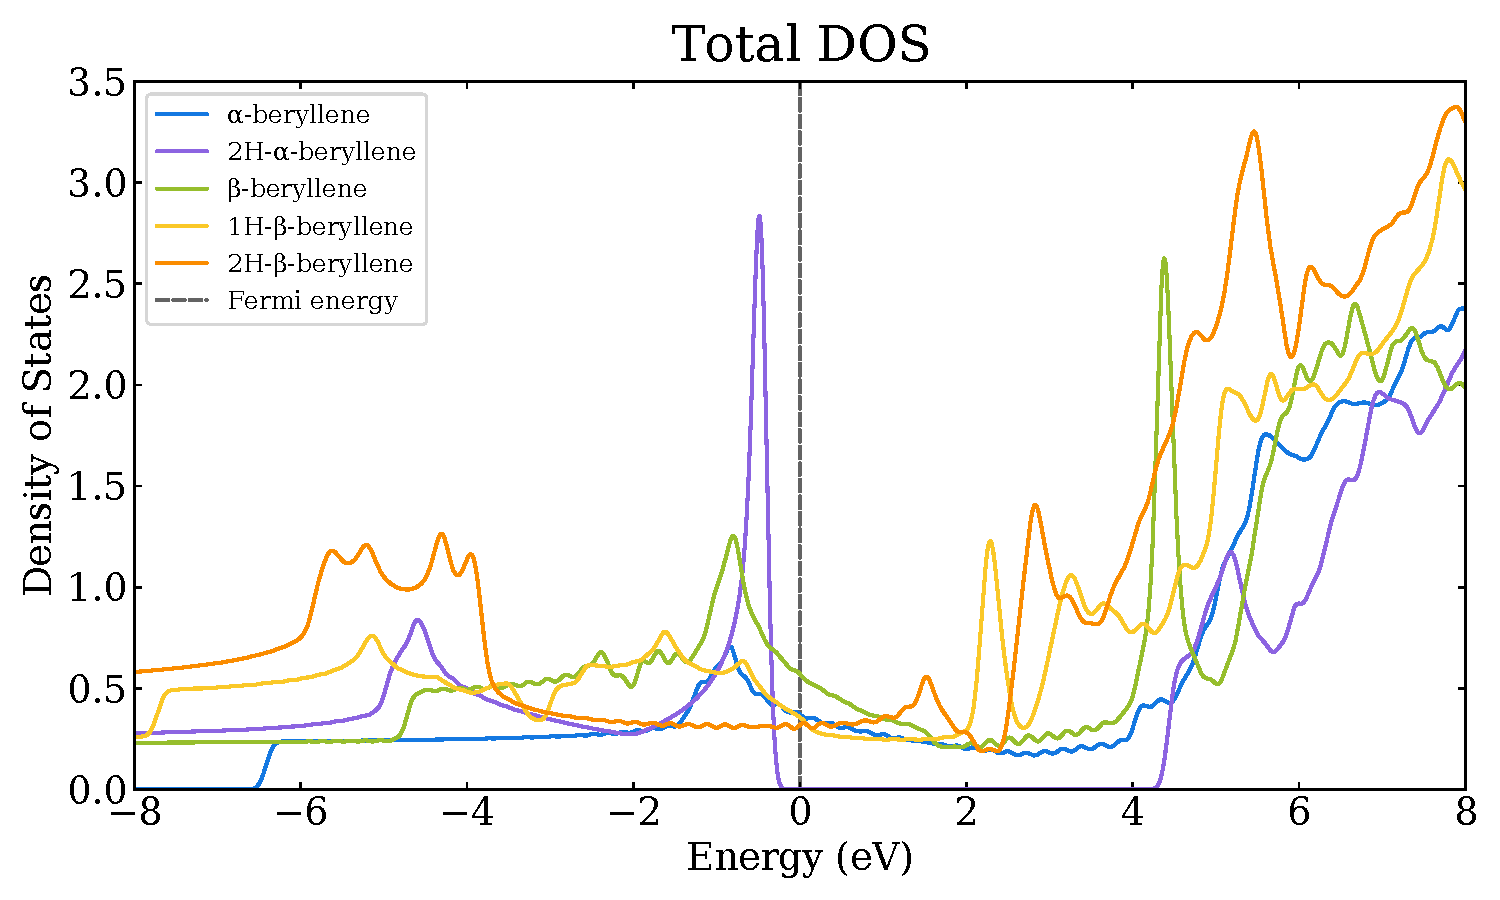
\includegraphics[width=0.40\linewidth]{figures_proj3/dos_hydrogenated_thesis.pdf}}&
    \adjustbox{valign=c}{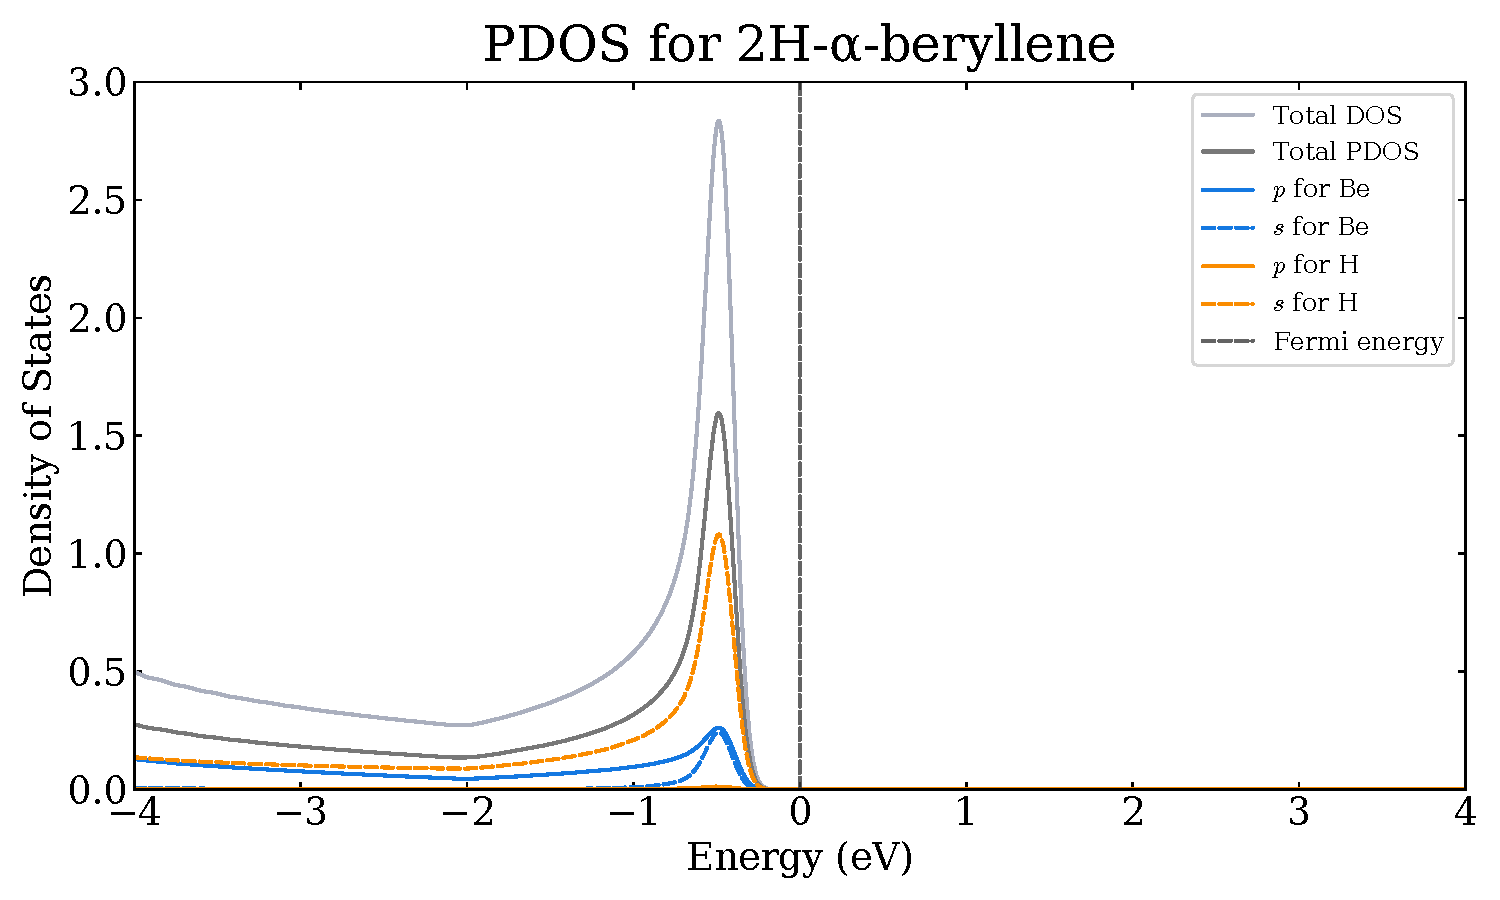
\includegraphics[width=0.40\linewidth]{figures_proj3/pdos_2H-alpha-beryllene_thesis.pdf}}\\
    \adjustbox{valign=c}{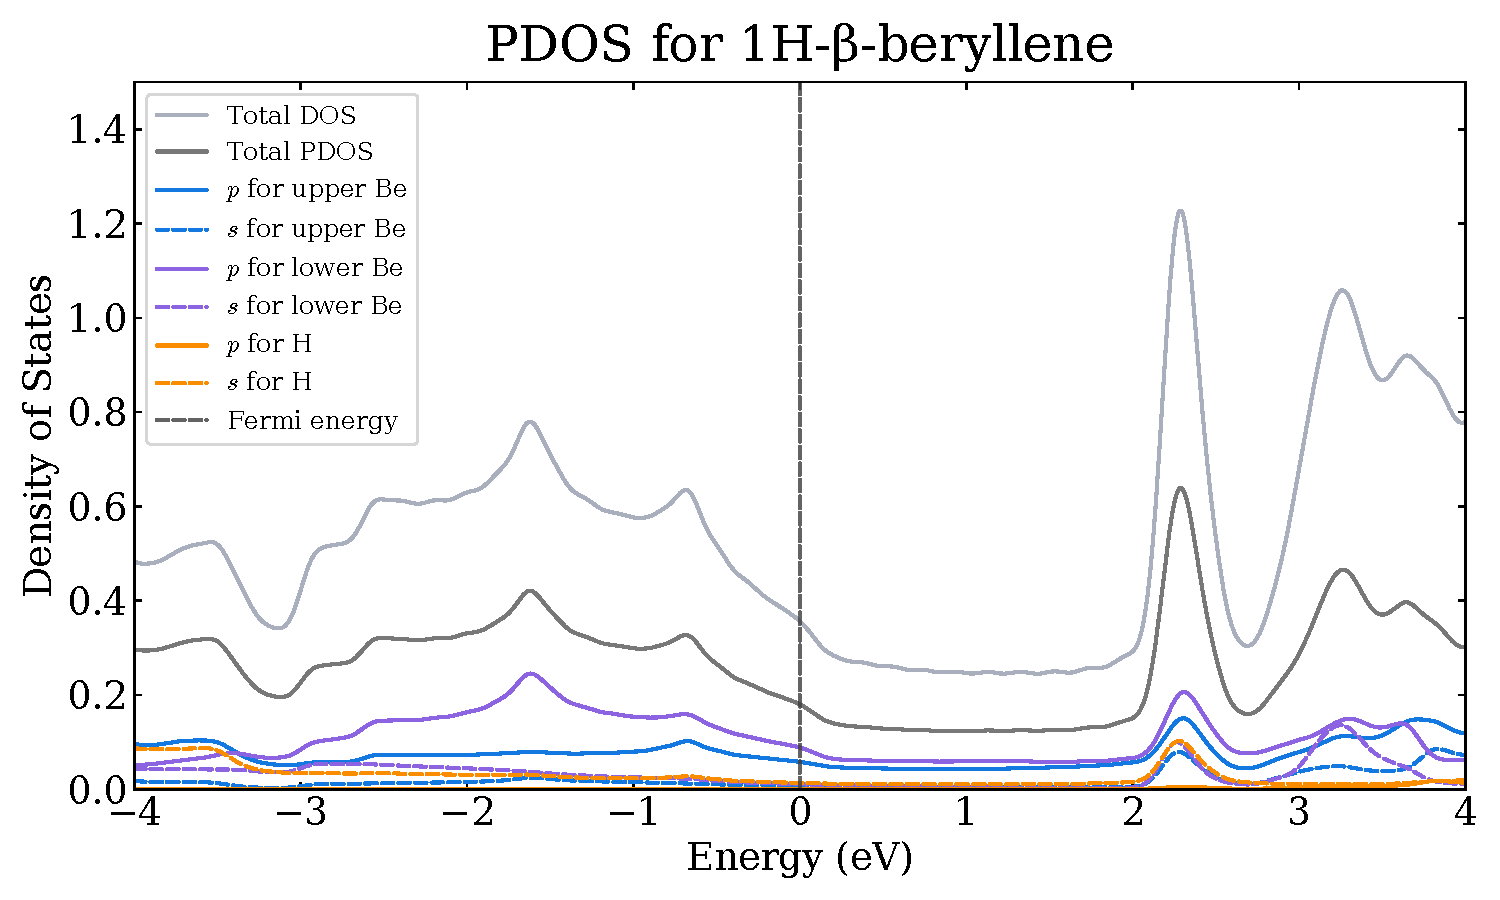
\includegraphics[width=0.40\linewidth]{figures_proj3/pdos_1H-beta-beryllene_thesis.pdf}}&
    \adjustbox{valign=c}{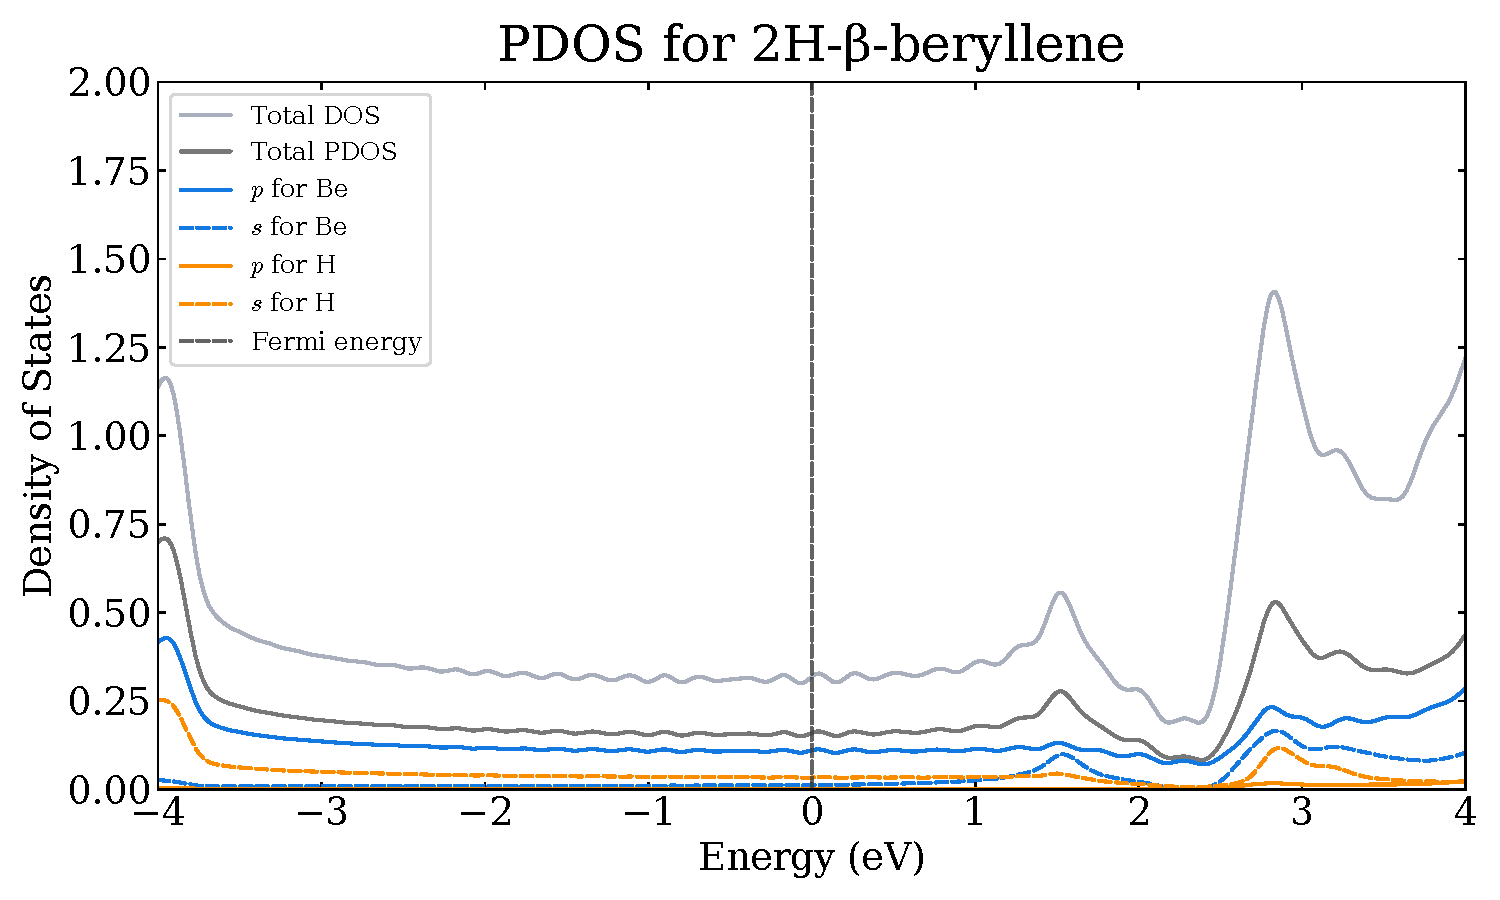
\includegraphics[width=0.40\linewidth]{figures_proj3/pdos_2H-beta-beryllene_thesis.pdf}}
\end{tabular}
\caption{Total and projected densities of states for pristine and hydrogen-functionalized beryllene structures.
Upper left: total density of states;
Upper right: projected density of states of 2H-$\alpha$-beryllene;
Lower left: projected density of states of 1H-$\beta$-beryllene;
Lower right: projected density of states of 2H-$\beta$-beryllene.}
\label{fig:proj3_dos_hydrogenated}
\end{figure}

\subsection{Topological properties}
\label{3_topological_properties}

Previous studies reported non-trivial topology in $\alpha$-beryllene,
whereas $\beta$-beryllene was classified as topologically trivial~\cite{li2023coexistence}.
Since $\alpha$-beryllene,
$\beta$-beryllene,
trilayer cubic beryllene,
2H-$\alpha$-beryllene,
and 2H-$\beta$-beryllene have inversion symmetry,
we verify their topological character using the $Z_{2}$ invariant calculated from the parity eigenvalues of the spin-orbit-coupled states at the time-reversal invariant momenta.
1H-$\beta$-beryllene has no inversion symmetry,
so its $Z_{2}$ invariant is obtained from the evolution of the Wannier charge centres~\cite{soluyanov2011computing,gresch2017z2pack}.

The calculation settings are described in section~\ref{3_methods}.
The $Z_{2}$ index $\nu$ follows from the parity products $\delta_i$ of the lowest $N$ spinor bands at the four time-reversal invariant momenta $\Gamma$,
$\mathrm{X}$,
$\mathrm{Y}$,
and $\mathrm{M}$,
according to equations~\eqref{eq:proj3_parity_product} and~\eqref{eq:proj3_z2_index},
where $N$ is the number of valence electrons per unit cell.

Except for 2H-$\alpha$-beryllene,
the structures considered here are metallic,
so the lowest $N$ bands are not completely filled.
In this case,
$\nu$ is defined for the subspace of the lowest $N$ bands only if this subspace is separated from band $N+1$ by a direct gap,
$E_{N+1}(\vec{k})-E_{N}(\vec{k})>0$,
at every $\vec{k}$ in the Brillouin zone.
The index then describes a band inversion within this subspace,
rather than a quantum spin Hall state at the Fermi level.
We therefore determine the minimum of this direct gap over the Brillouin zone,
as described in section~\ref{3_methods}.
Since these gaps are sampled rather than proven on the continuous Brillouin zone,
and since the analysis assumes time-reversal symmetry,
the resulting $Z_{2}$ indices are conditional screening results.

The calculated parity eigenvalues,
parity products,
$Z_{2}$ indices,
and minimum direct gaps are listed in table~\ref{tab:proj3_topological_parity}.
For $\alpha$-beryllene,
$\beta$-beryllene,
and 2H-$\alpha$-beryllene,
the $\mathrm{X}$,
$\mathrm{Y}$,
and $\mathrm{M}$ points correspond to the three $\mathrm{M}$ points of the hexagonal Brillouin zone,
which are equivalent by symmetry,
so the Fu--Kane product reduces to
$(-1)^{\nu}=\delta_{\Gamma}(\delta_{\mathrm{M}})^3=\delta_{\Gamma}\delta_{\mathrm{M}}$.
For trilayer cubic beryllene,
the $\mathrm{X}$ and $\mathrm{Y}$ points are the two equivalent $\mathrm{X}$ points of the square Brillouin zone,
which contribute as $(\delta_{\mathrm{X}})^2$,
and the product reduces to
$(-1)^{\nu}=\delta_{\Gamma}\delta_{\mathrm{M}}(\delta_{\mathrm{X}})^2=\delta_{\Gamma}\delta_{\mathrm{M}}$.
For 2H-$\beta$-beryllene,
the four time-reversal invariant momenta are not all equivalent,
and the parity products at all four points are used.

\begin{table}[!htbp]
\centering
\rowcolors{2}{gray!15}{white}
\setlength{\tabcolsep}{8pt}
\begin{adjustbox}{max width=1.0\linewidth,center}
\begin{tabular}{ccccccccc}
\hline
\rowcolor{gray!25}
structure
& $N$
& $\Gamma$
& $\mathrm{X}$
& $\mathrm{Y}$
& $\mathrm{M}$
& product
& $\nu$
& min. direct gap \\
\hline
$\alpha$-beryllene
& 2
& $+$
& $-$
& $-$
& $-$
& $-1$
& 1
& \qty{1.13}{\milli\electronvolt} \\
$\beta$-beryllene
& 4
& $+, -$
& $+, -$
& $+, -$
& $+, -$
& $+1$
& 0
& \qty{0.898}{\milli\electronvolt} \\
trilayer cubic beryllene
& 6
& $+, -, +$
& $+, -, +$
& $+, -, +$
& $-, -, +$
& $-1$
& 1
& \qty{0.735}{\milli\electronvolt} \\
2H-$\alpha$-beryllene
& 4
& $+, -$
& $-, +$
& $-, +$
& $-, +$
& $+1$
& 0
& \qty{4.92}{\electronvolt} \\
2H-$\beta$-beryllene
& 6
& $+, -, +$
& $-, +, +$
& $+, -, -$
& $-, +, -$
& $+1$
& 0
& \qty{0.177}{\electronvolt} \\
1H-$\beta$-beryllene
& 4 / 6
& --
& --
& --
& --
& --
& 0 / 0
& 0.929 / \qty{0.415}{\electronvolt} \\
\hline
\end{tabular}
\end{adjustbox}
\caption{Parity eigenvalues of the Kramers pairs of the lowest $N$ spinor bands at the time-reversal invariant momenta,
listed from the lowest pair upward,
Fu--Kane products,
$Z_{2}$ indices,
and minimum direct gaps $E_{N+1}-E_{N}$ over the Brillouin zone.
For 1H-$\beta$-beryllene,
which has no inversion symmetry,
the $Z_{2}$ indices of the lowest four and lowest six bands are obtained from the Wannier charge centres.}
\label{tab:proj3_topological_parity}
\end{table}

For $\alpha$-beryllene,
the single Kramers pair is even at the $\Gamma$ point and odd at the three zone-boundary points.
The Fu--Kane product is therefore $(-1)^{\nu}=-1$,
which gives $\nu=1$ and confirms the non-trivial topology previously reported for this phase.
These two bands are separated from band 3 at every sampled wave vector,
and the smallest separation is the spin-orbit gap of \qty{1.13}{\milli\electronvolt} at the Dirac point at $\mathrm{K}$,
approximately \qty{2.7}{\electronvolt} above the Fermi level.
For $\beta$-beryllene,
the parity products give $(-1)^{\nu}=+1$,
which gives $\nu=0$ and confirms that this phase is topologically trivial.
Its smallest direct gap is the spin-orbit gap of \qty{0.898}{\milli\electronvolt} at $\mathrm{K}$.
For trilayer cubic beryllene,
the parity products again change sign between the $\Gamma$ and $\mathrm{M}$ points,
giving $(-1)^{\nu}=-1$ and $\nu=1$.
At $\mathrm{M}$,
the next Kramers pair lies only \qty{1.3}{\milli\electronvolt} above band 6,
but it has the same parity as bands 5 and 6,
so the order of these two pairs does not change $\nu$.
The smallest direct gap of \qty{0.735}{\milli\electronvolt} occurs at a spin-orbit-gapped crossing on the $\Gamma$--$\mathrm{M}$ line.
Therefore,
trilayer cubic beryllene is also a non-trivial $Z_{2}$ topological phase,
in the same conditional sense as $\alpha$-beryllene.

Both $\alpha$-beryllene and trilayer cubic beryllene are metallic at the neutral Fermi level,
and their non-trivial subspaces are isolated only by spin-orbit gaps of approximately \qty{1}{\milli\electronvolt},
located \qtyrange{1.2}{2.7}{\electronvolt} above the Fermi level.
The non-trivial index therefore characterizes a band inversion rather than a quantum spin Hall insulating state.
Gaps of this size are also far below the accuracy of the band ordering in semilocal density functional theory,
so this result may be sensitive to the exchange-correlation functional.

Hydrogen functionalization gives trivial $Z_{2}$ indices in all three structures.
2H-$\alpha$-beryllene is the only insulator among the structures considered,
so its index $\nu=0$ classifies the occupied bands at the Fermi level.
For 2H-$\beta$-beryllene,
$\nu=0$,
and the smallest direct gap of \qty{0.177}{\electronvolt} occurs near $\mathrm{M}$.
1H-$\beta$-beryllene has five valence electrons per unit cell,
so its Fermi level lies within the half-filled fifth and sixth bands.
Its lowest four and lowest six bands are separated from the next bands by minimum direct gaps of \qty{0.929}{\electronvolt} and \qty{0.415}{\electronvolt},
respectively,
and the Wannier charge centres give $Z_{2}=0$ for both subspaces.

The parity eigenvalues at the four time-reversal invariant momenta are unchanged when the HSE06 hybrid functional is used without spin-orbit coupling,
so the $\nu$ values of the five centrosymmetric structures remain the same with this functional.
This check tests the band order at the time-reversal invariant momenta,
but not the spin-orbit gaps of approximately \qty{1}{\milli\electronvolt} elsewhere in the Brillouin zone.
The converged spin-orbit-coupled states are nonmagnetic,
with a magnetization density below $3\times10^{-7}~\mu_{\mathrm{B}}\,\text{\AA}^{-3}$,
and spin-polarized calculations started from ferromagnetic and antiferromagnetic configurations all converge to the nonmagnetic state.
These results support the time-reversal symmetry assumed in the analysis.
The band structures with the lowest-$N$ subspaces are shown in figures~\ref{fig:proj3_topology_bands_pristine} and~\ref{fig:proj3_topology_bands_hydrogenated}.
The direct-gap maps,
the refinement of the smallest gaps,
and the Wannier charge centres of 1H-$\beta$-beryllene are shown in figures~\ref{fig:proj3_direct_gap_pristine}--\ref{fig:proj3_wcc},
and the HSE06 parities are listed in table~\ref{tab:proj3_hse_parity} in section~\ref{3_supplementary}.

\begin{figure}[!htbp]
\centering
    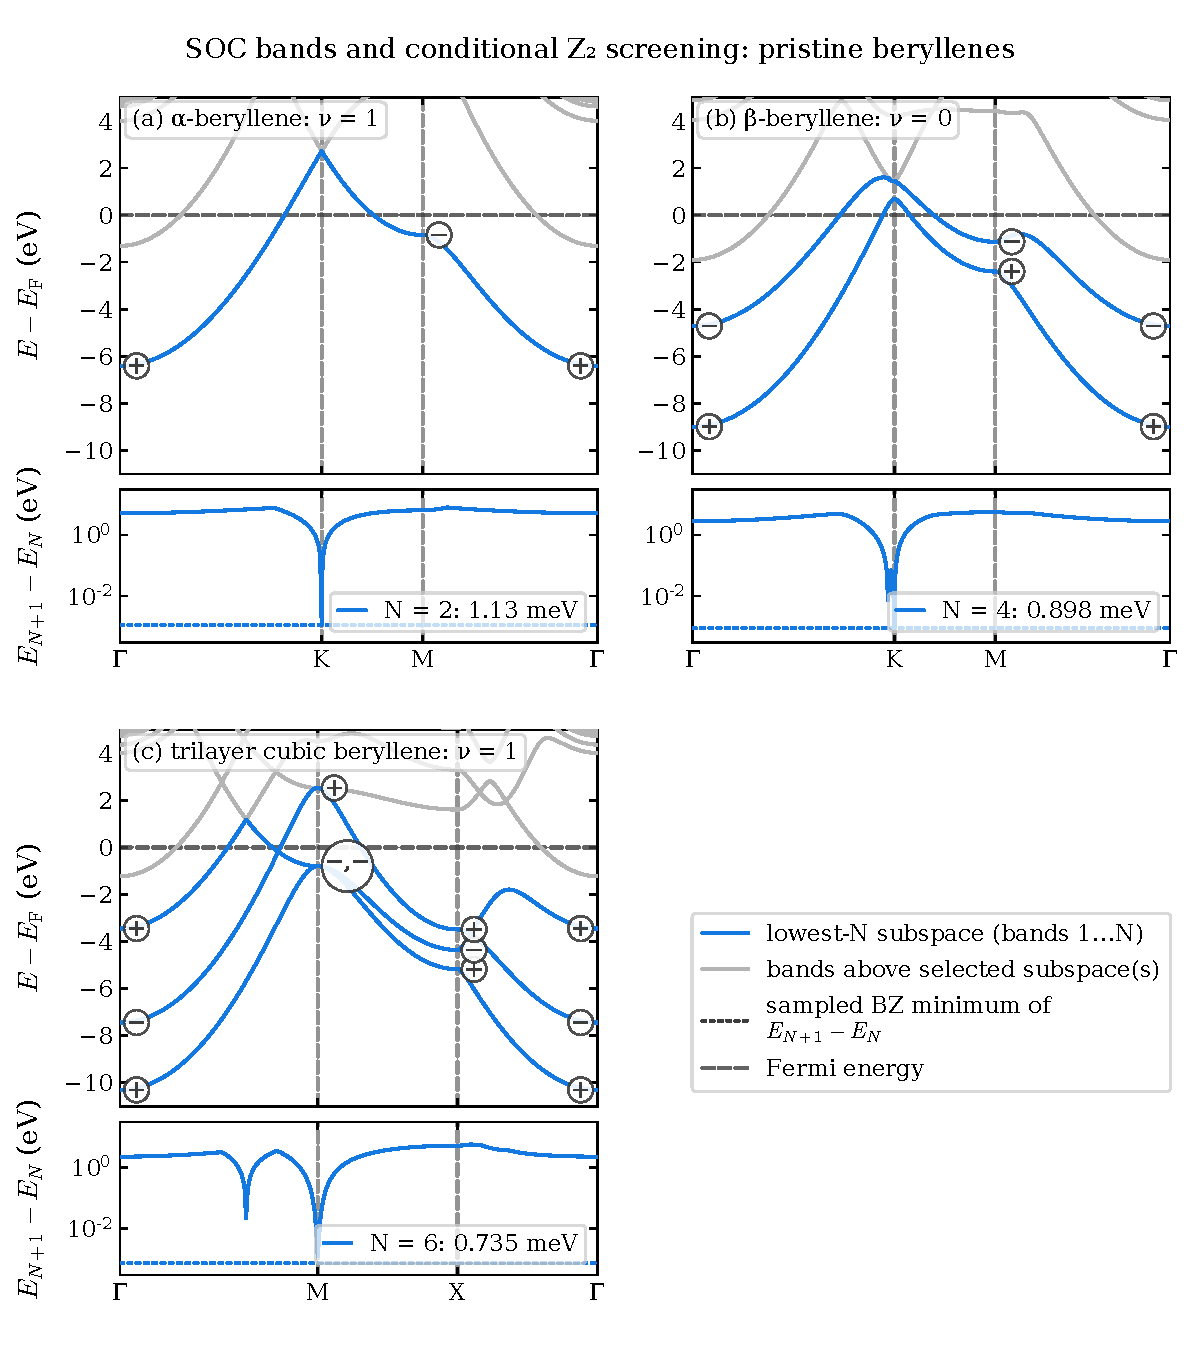
\includegraphics[width=0.80\linewidth]{figures_proj3/topology_bands_pristine_thesis.pdf}
\caption{Spin-orbit-coupled band structures of $\alpha$-beryllene,
$\beta$-beryllene,
and trilayer cubic beryllene.
The lowest $N$ bands are shown in blue,
and the parities of their Kramers pairs are marked at the time-reversal invariant momenta on the path,
where pairs within \qty{0.45}{\electronvolt} of each other share one marker and are listed from the lowest pair upward.
Below each band structure,
the direct gap $E_{N+1}-E_{N}$ along the path is shown on a logarithmic scale,
together with its minimum over the Brillouin zone.}
\label{fig:proj3_topology_bands_pristine}
\end{figure}

\begin{figure}[!htbp]
\centering
    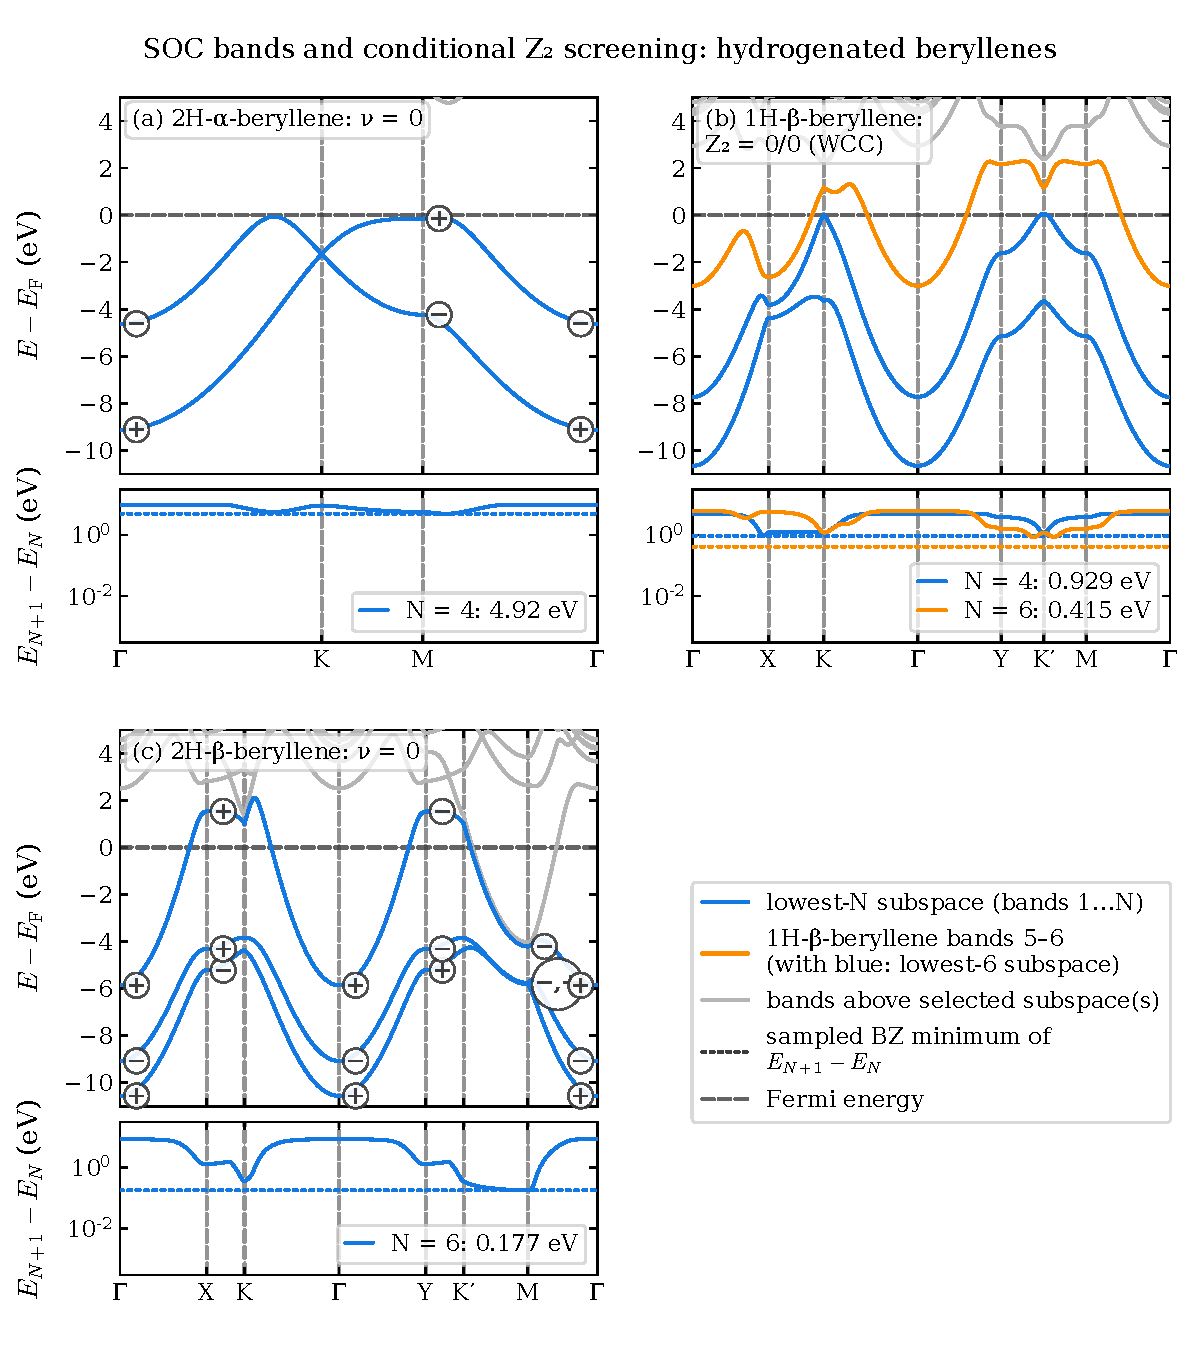
\includegraphics[width=0.80\linewidth]{figures_proj3/topology_bands_hydrogenated_thesis.pdf}
\caption{Spin-orbit-coupled band structures of 2H-$\alpha$-beryllene,
1H-$\beta$-beryllene,
and 2H-$\beta$-beryllene,
shown as in figure~\ref{fig:proj3_topology_bands_pristine}.
For 1H-$\beta$-beryllene,
bands 1--4 are shown in blue and bands 5 and 6 in orange,
corresponding to the lowest-four and lowest-six subspaces.
For 1H-$\beta$-beryllene and 2H-$\beta$-beryllene,
the path is the same as in figure~\ref{fig:proj3_band_structures_cubic_hydrogenated}.}
\label{fig:proj3_topology_bands_hydrogenated}
\end{figure}

\subsection{Optical properties}
\label{3_optical_properties}

We now examine the optical properties of the pristine and hydrogen-functionalized beryllene structures,
together with the bulk hcp and bulk bcc beryllium reference phases.
The dielectric function,
absorption coefficient,
refractive index,
extinction coefficient,
reflectivity,
and energy-loss spectrum are defined in chapter~\ref{cha:fundamentals_b},
especially sections~\ref{sec:from_electronic_response_to_dielectric_function} and~\ref{sec:from_dielectric_function_to_optical_properties}.
Here,
we use these quantities to compare the direction-dependent optical response of the beryllene structures.

\subsubsection{Pristine $\alpha$- and $\beta$-beryllene}
\label{3_optical_alpha_beta}

We first discuss the optical response of pristine $\alpha$-beryllene and $\beta$-beryllene,
which then provides a reference for bulk beryllium,
trilayer cubic beryllene,
and the hydrogen-functionalized structures.
The real and imaginary parts of the dielectric function for the in-plane and out-of-plane directions are shown in figure~\ref{fig:proj3_alpha_beta_dielectric}.

For $\beta$-beryllene,
the in-plane real part contains zero crossings and a low-energy interval in which its sign differs from the out-of-plane component.
On the calculated grid, these components have opposite signs from approximately \qtyrange{1.22}{2.21}{\electronvolt};
these are sampled endpoints rather than interpolated zeros.
For $\alpha$-beryllene, the out-of-plane real part crosses zero near \qty{10.64}{\electronvolt}, where the imaginary part is comparatively small.
The sign changes and loss features identify candidate energy ranges for further analysis of collective response.
They do not by themselves establish propagating modes in a finite two-dimensional layer or determine their lifetimes.
The numerical broadening is an input to the calculation, not a calculated scattering lifetime.

\begin{figure}[!htbp]
\centering
    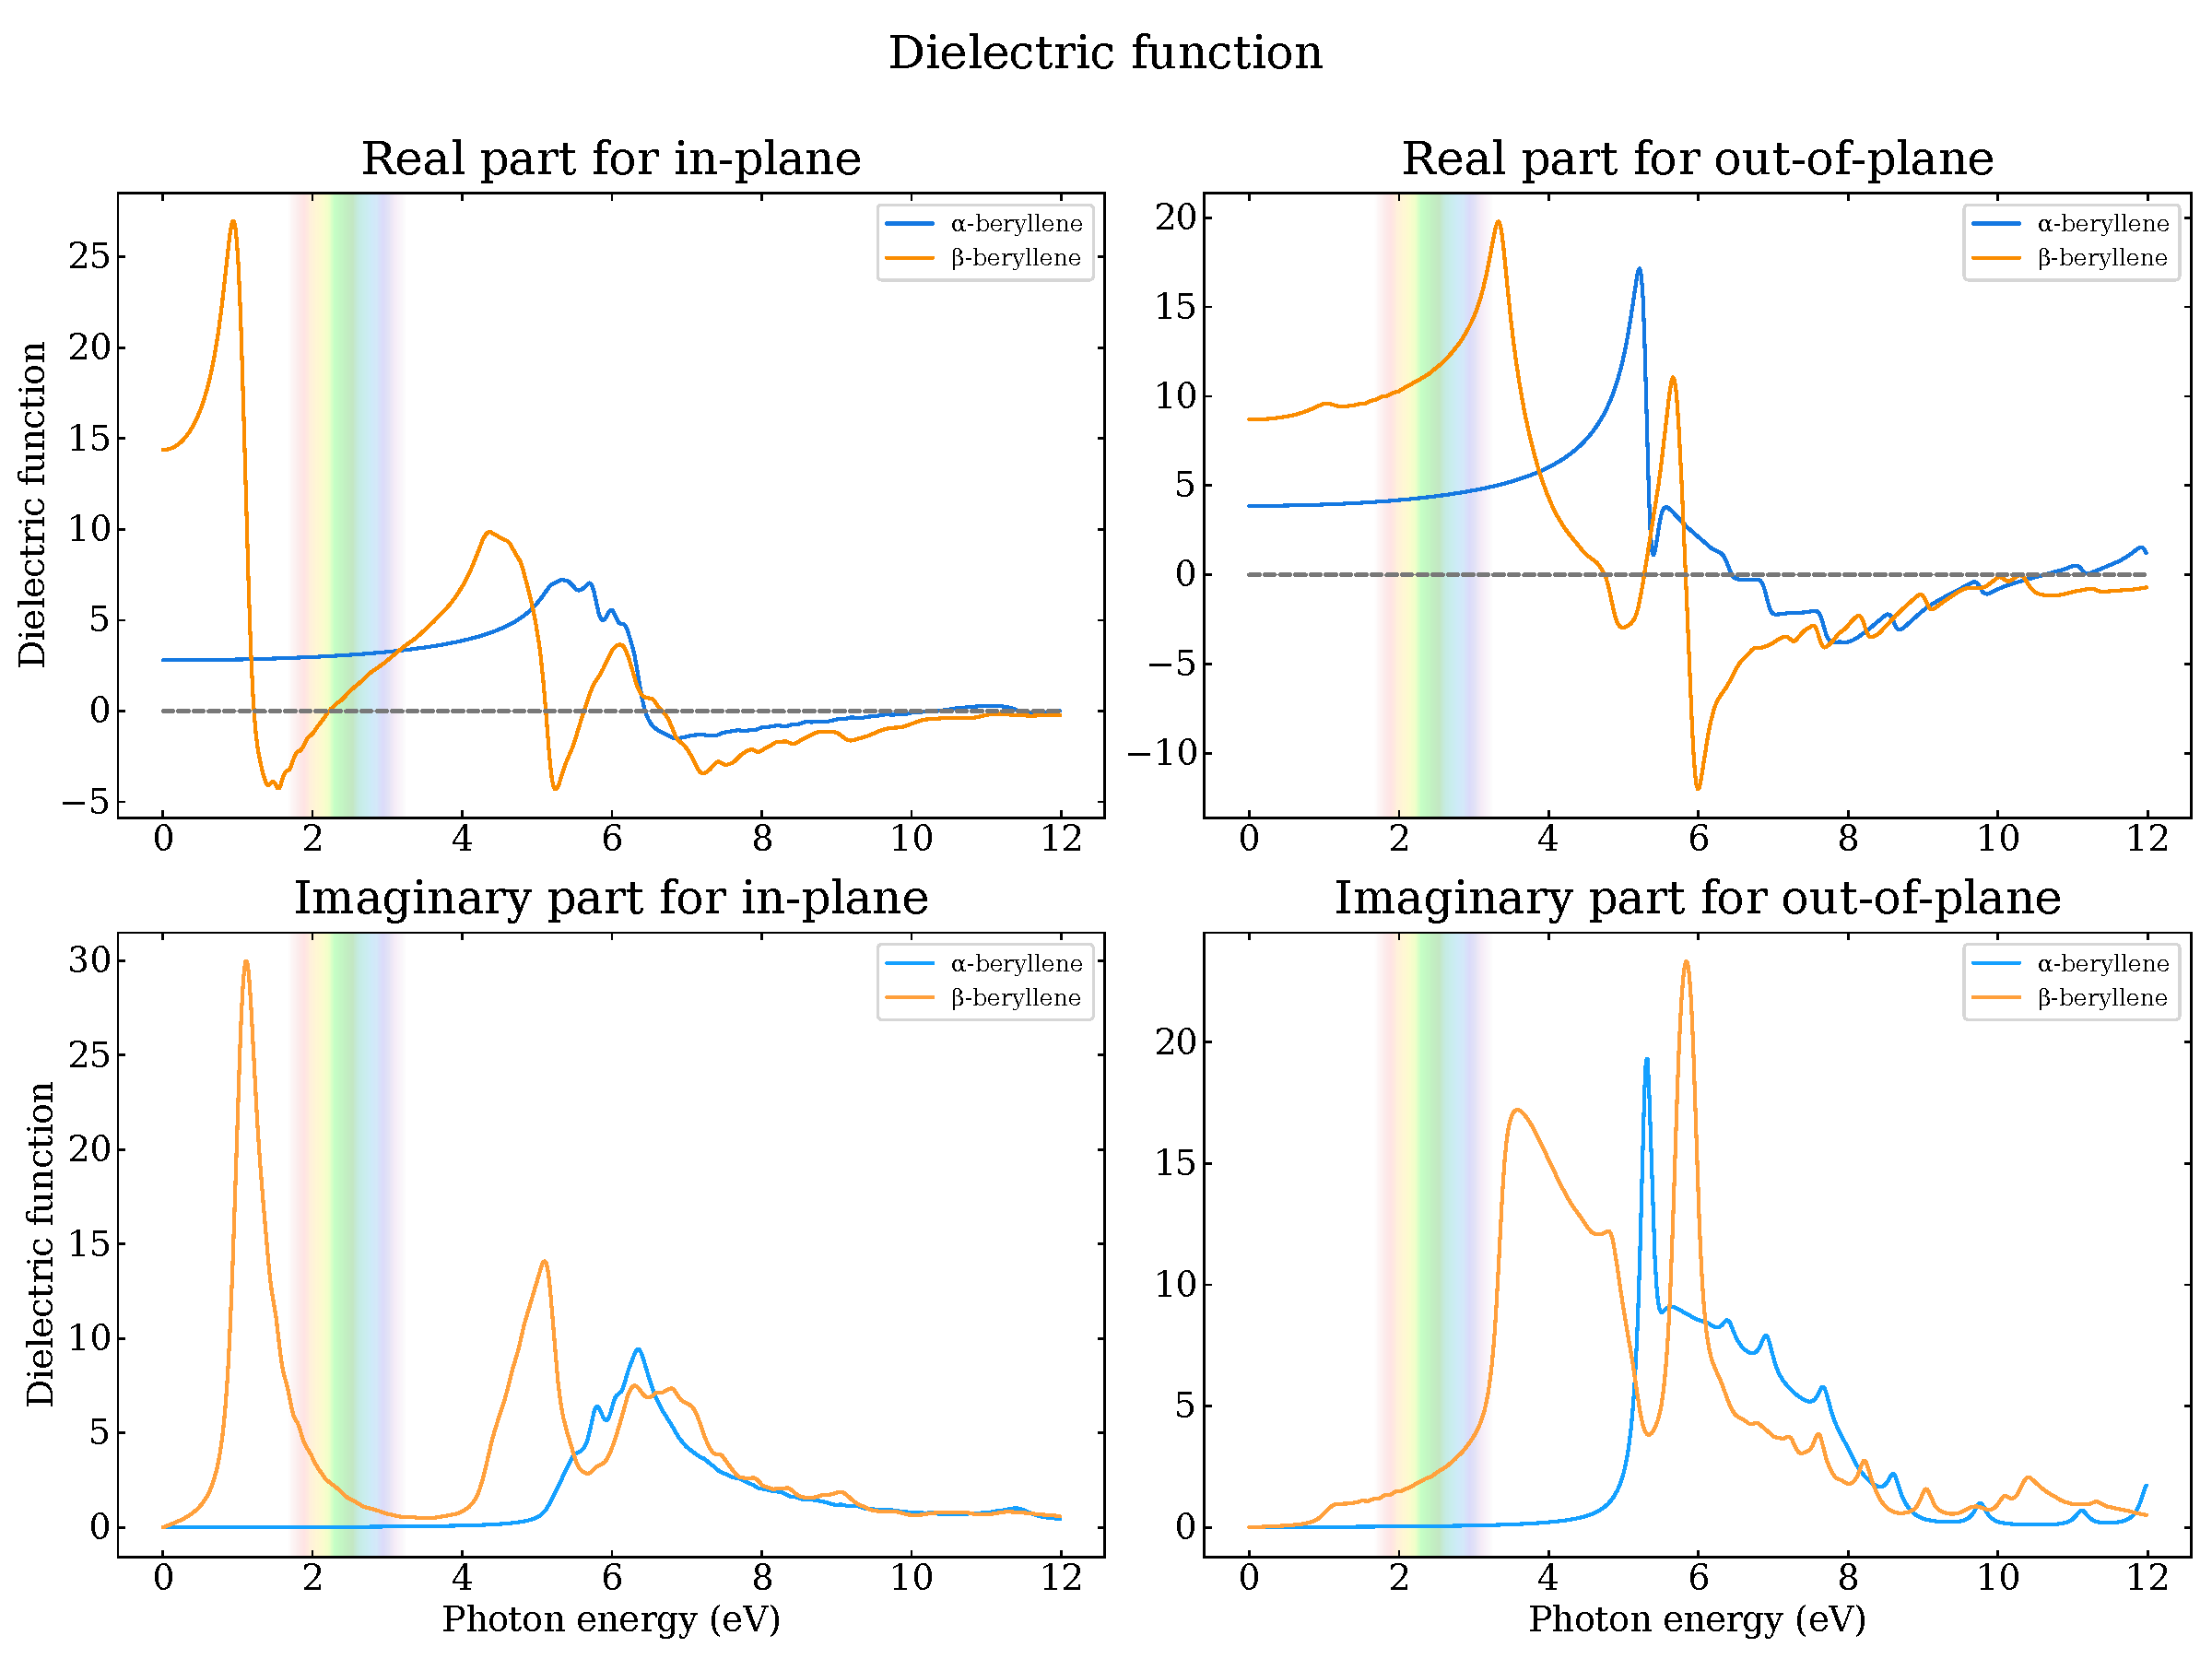
\includegraphics[width=0.80\linewidth]{figures_proj3/dielectric_alpha-beta_thesis.pdf}
\caption{Real and imaginary parts of the dielectric function for $\alpha$-beryllene and $\beta$-beryllene.
The spectra are shown for the in-plane and out-of-plane directions as functions of photon energy.
The in-plane and out-of-plane curves correspond to the $xx$ and $zz$ components, respectively.}
\label{fig:proj3_alpha_beta_dielectric}
\end{figure}

The absorption coefficient and refractive index are shown in figure~\ref{fig:proj3_alpha_beta_abs_refractive}.
The effective absorption is strongly anisotropic.
Within the \qtyrange{0}{12}{\electronvolt} window, the largest sampled coefficients for $\alpha$-beryllene are approximately
\qty{0.135}{\per\nano\metre} in $xx$ and \qty{0.175}{\per\nano\metre} in $zz$;
the corresponding $\beta$-beryllene values are approximately \qty{0.161}{\per\nano\metre} and \qty{0.242}{\per\nano\metre}.
The strongest $\beta$ out-of-plane feature occurs near \qty{5.95}{\electronvolt}.
The spectra cross at some energies, so the larger maxima do not imply that $\beta$-beryllene absorbs more strongly at every energy.

The refractive index spectra follow the same structural and directional contrast.
In the in-plane channel,
$\beta$-beryllene develops two pronounced enhancements in the infrared and near-ultraviolet regions,
with a minimum in the visible range.
By contrast,
$\alpha$-beryllene varies more smoothly over the same energy interval.
In the out-of-plane channel,
$\beta$-beryllene remains stronger than $\alpha$-beryllene over the infrared to near-ultraviolet range.
The first downward $n=1$ crossings occur near \qty{7.42}{\electronvolt} for $\alpha$ $xx$,
\qty{7.82}{\electronvolt} for $\alpha$ $zz$, \qty{7.32}{\electronvolt} for $\beta$ $xx$ and \qty{6.37}{\electronvolt} for $\beta$ $zz$.
The $\alpha$ out-of-plane index rises above one again near \qty{11.71}{\electronvolt}.
These crossings describe dispersion of the effective optical constants and do not by themselves identify a plasmon resonance.

\begin{figure}[!htbp]
\centering
    \adjustbox{valign=c}{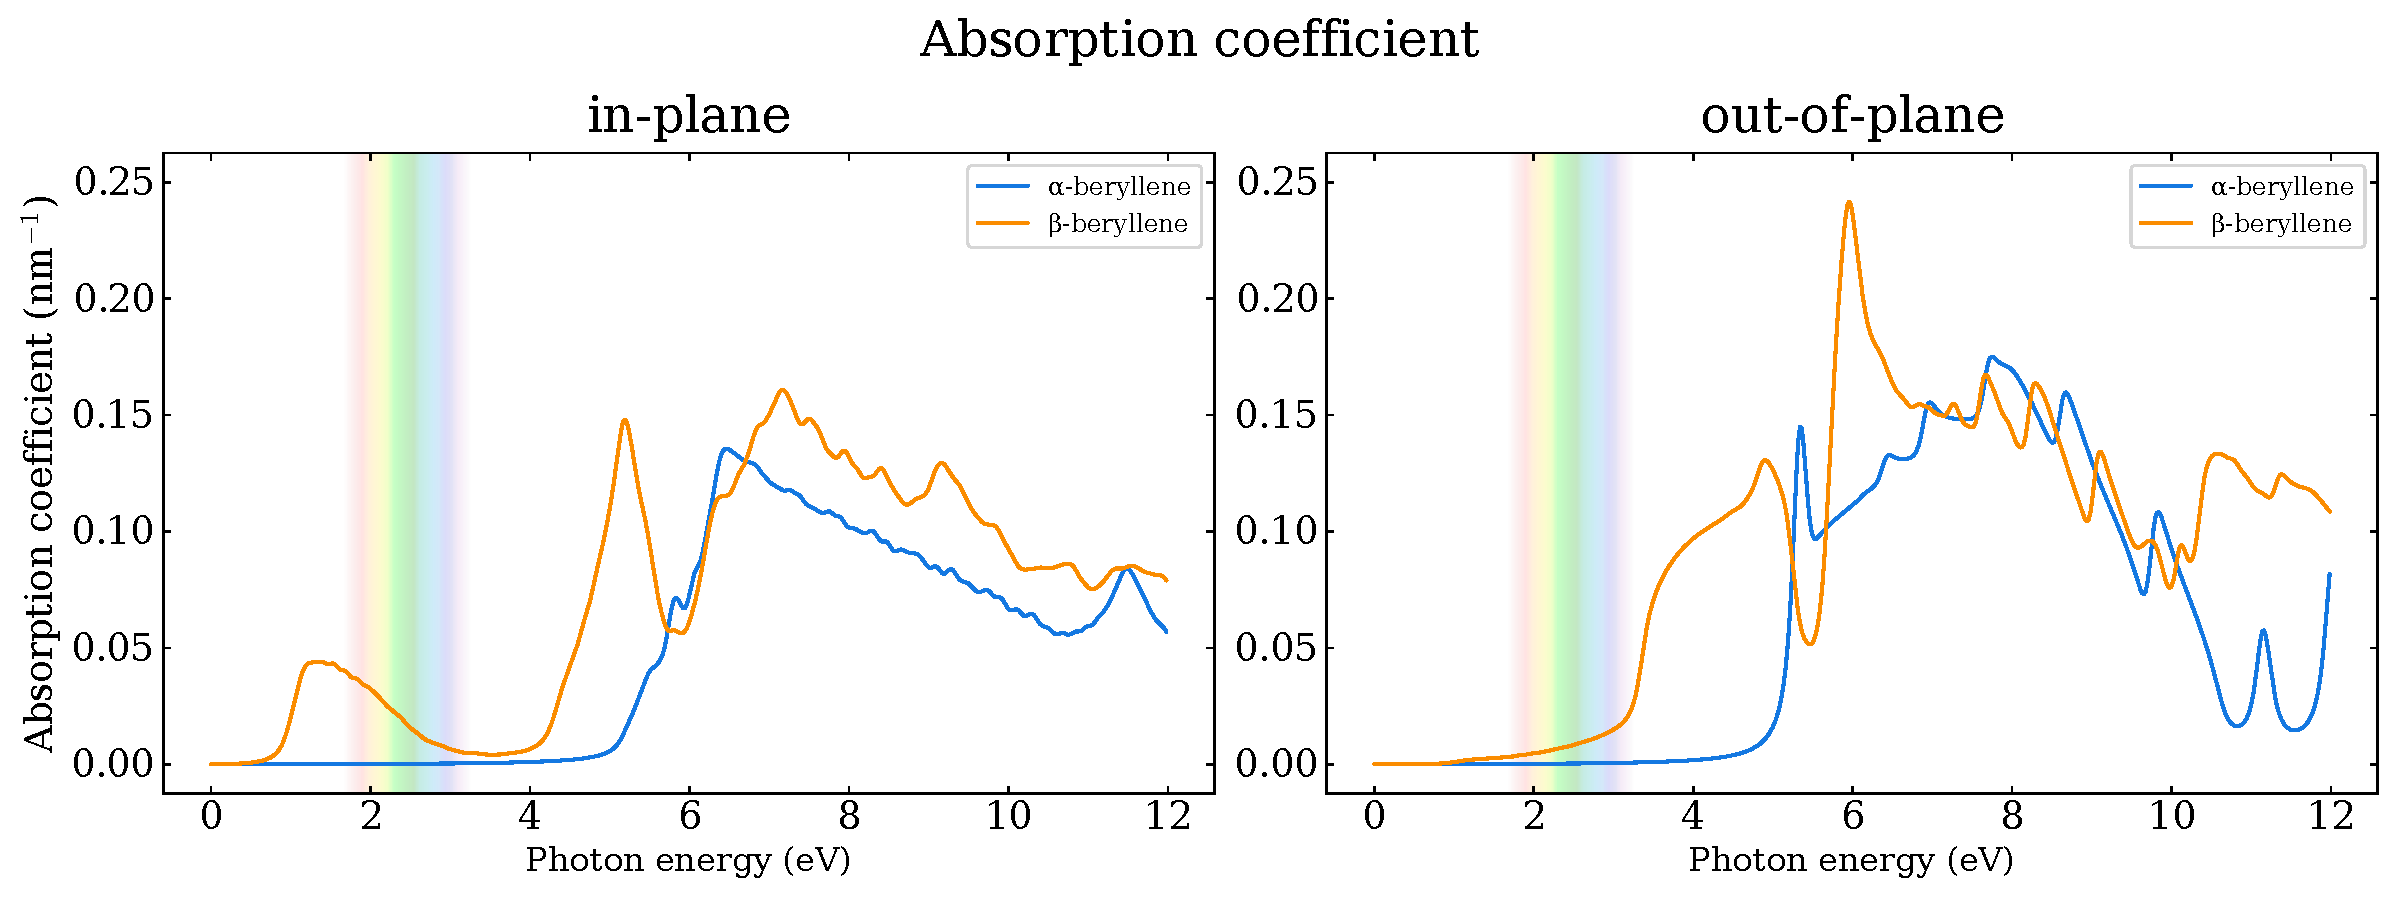
\includegraphics[width=0.80\linewidth]{figures_proj3/optics_alpha-beta_absorption_thesis.pdf}}%
    \par\nointerlineskip
    \adjustbox{valign=c}{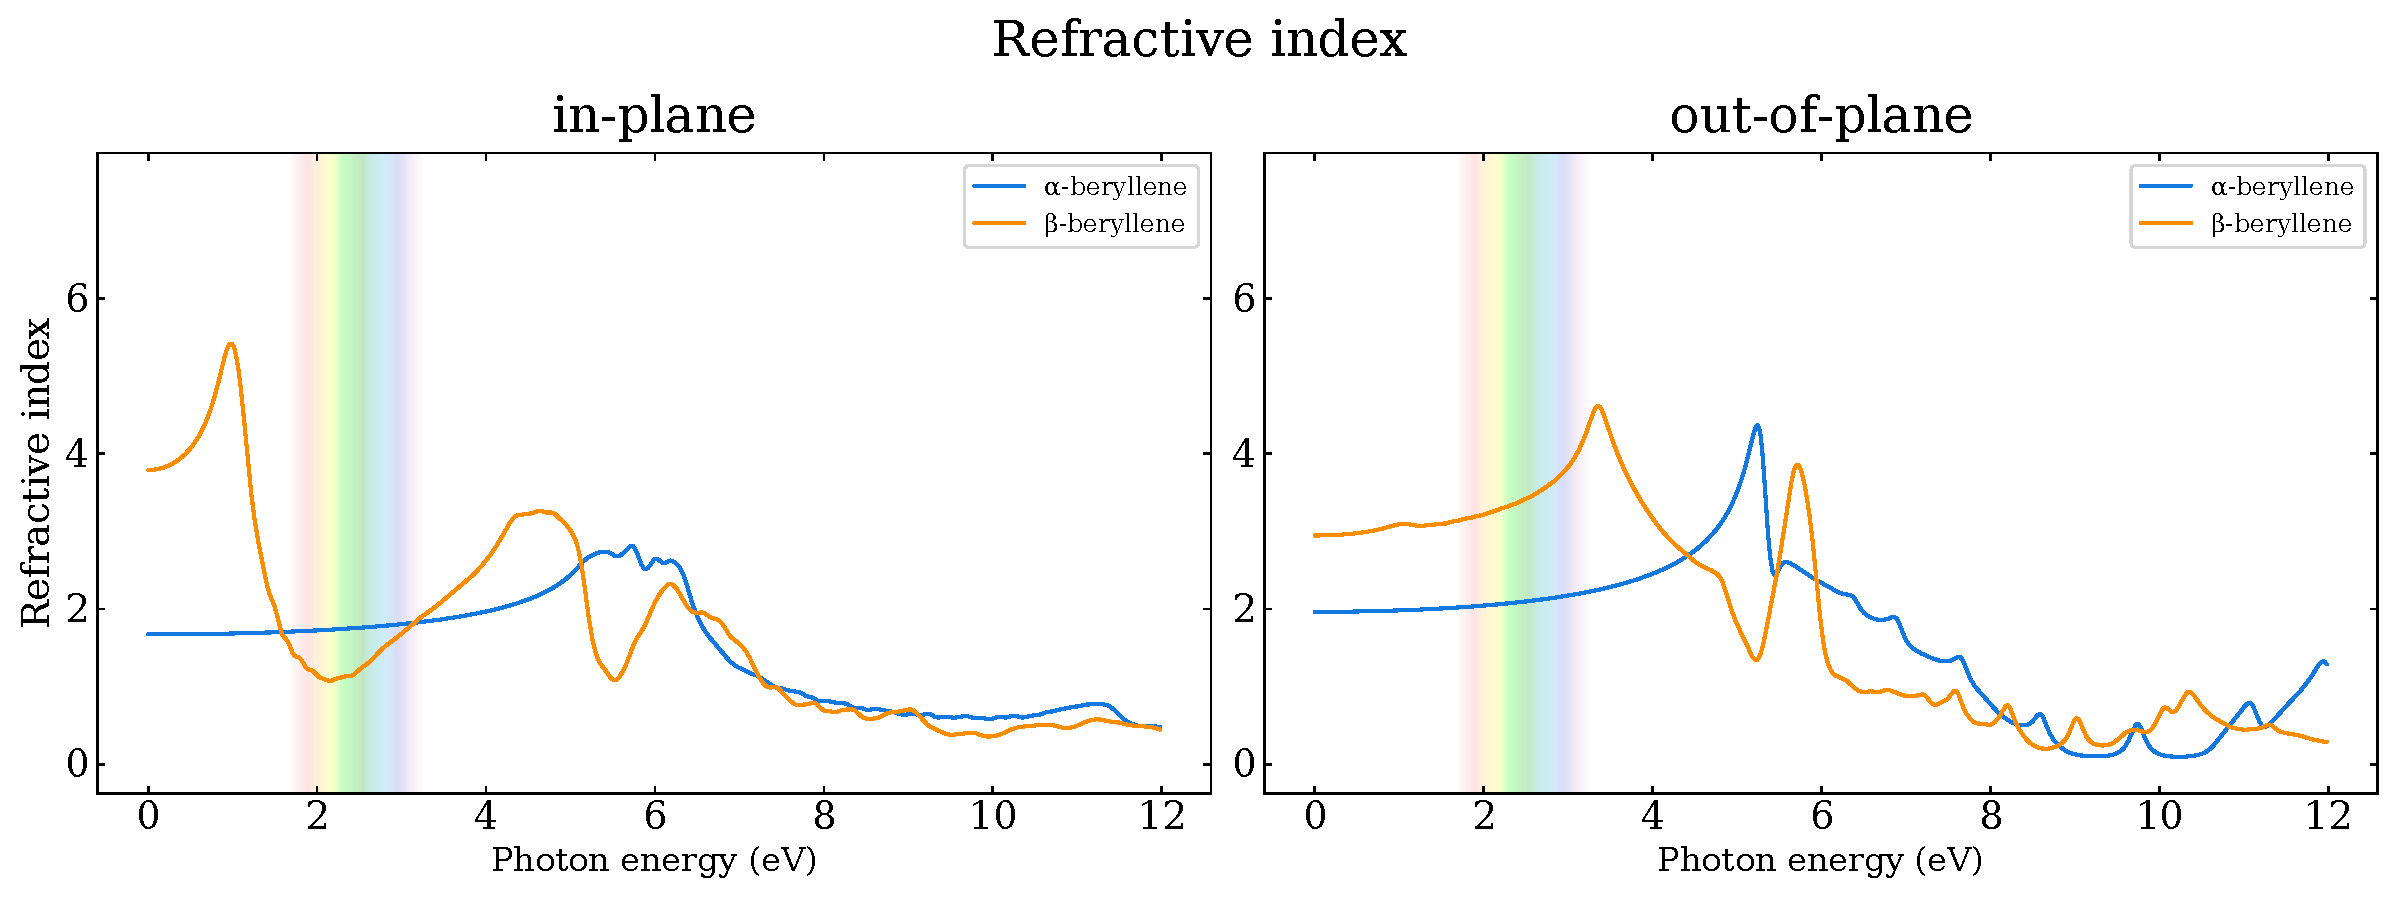
\includegraphics[width=0.80\linewidth]{figures_proj3/optics_alpha-beta_refractive_thesis.pdf}}%
\caption{Absorption coefficient and refractive index of $\alpha$-beryllene and $\beta$-beryllene.
Upper: absorption coefficient ($\mathrm{nm}^{-1}$); Lower: refractive index.
The spectra are shown for the in-plane and out-of-plane directions as functions of photon energy.
The in-plane and out-of-plane curves correspond to the $xx$ and $zz$ components, respectively.}
\label{fig:proj3_alpha_beta_abs_refractive}
\end{figure}

The extinction coefficient is shown in figure~\ref{fig:proj3_alpha_beta_extinction}.
In the in-plane channel,
$\beta$-beryllene develops strong peaks in the infrared and near-ultraviolet regions,
separated by a pronounced trough.
By contrast,
$\alpha$-beryllene again varies more smoothly.
In the out-of-plane channel,
$\beta$-beryllene develops its strongest extinction peak near \qty{5.95}{\electronvolt}, where $k\approx4.00$, followed by weaker higher-energy features.
This behaviour shows that amplitude attenuation also depends on both optical direction and crystal structure.

\begin{figure}[!htbp]
\centering
    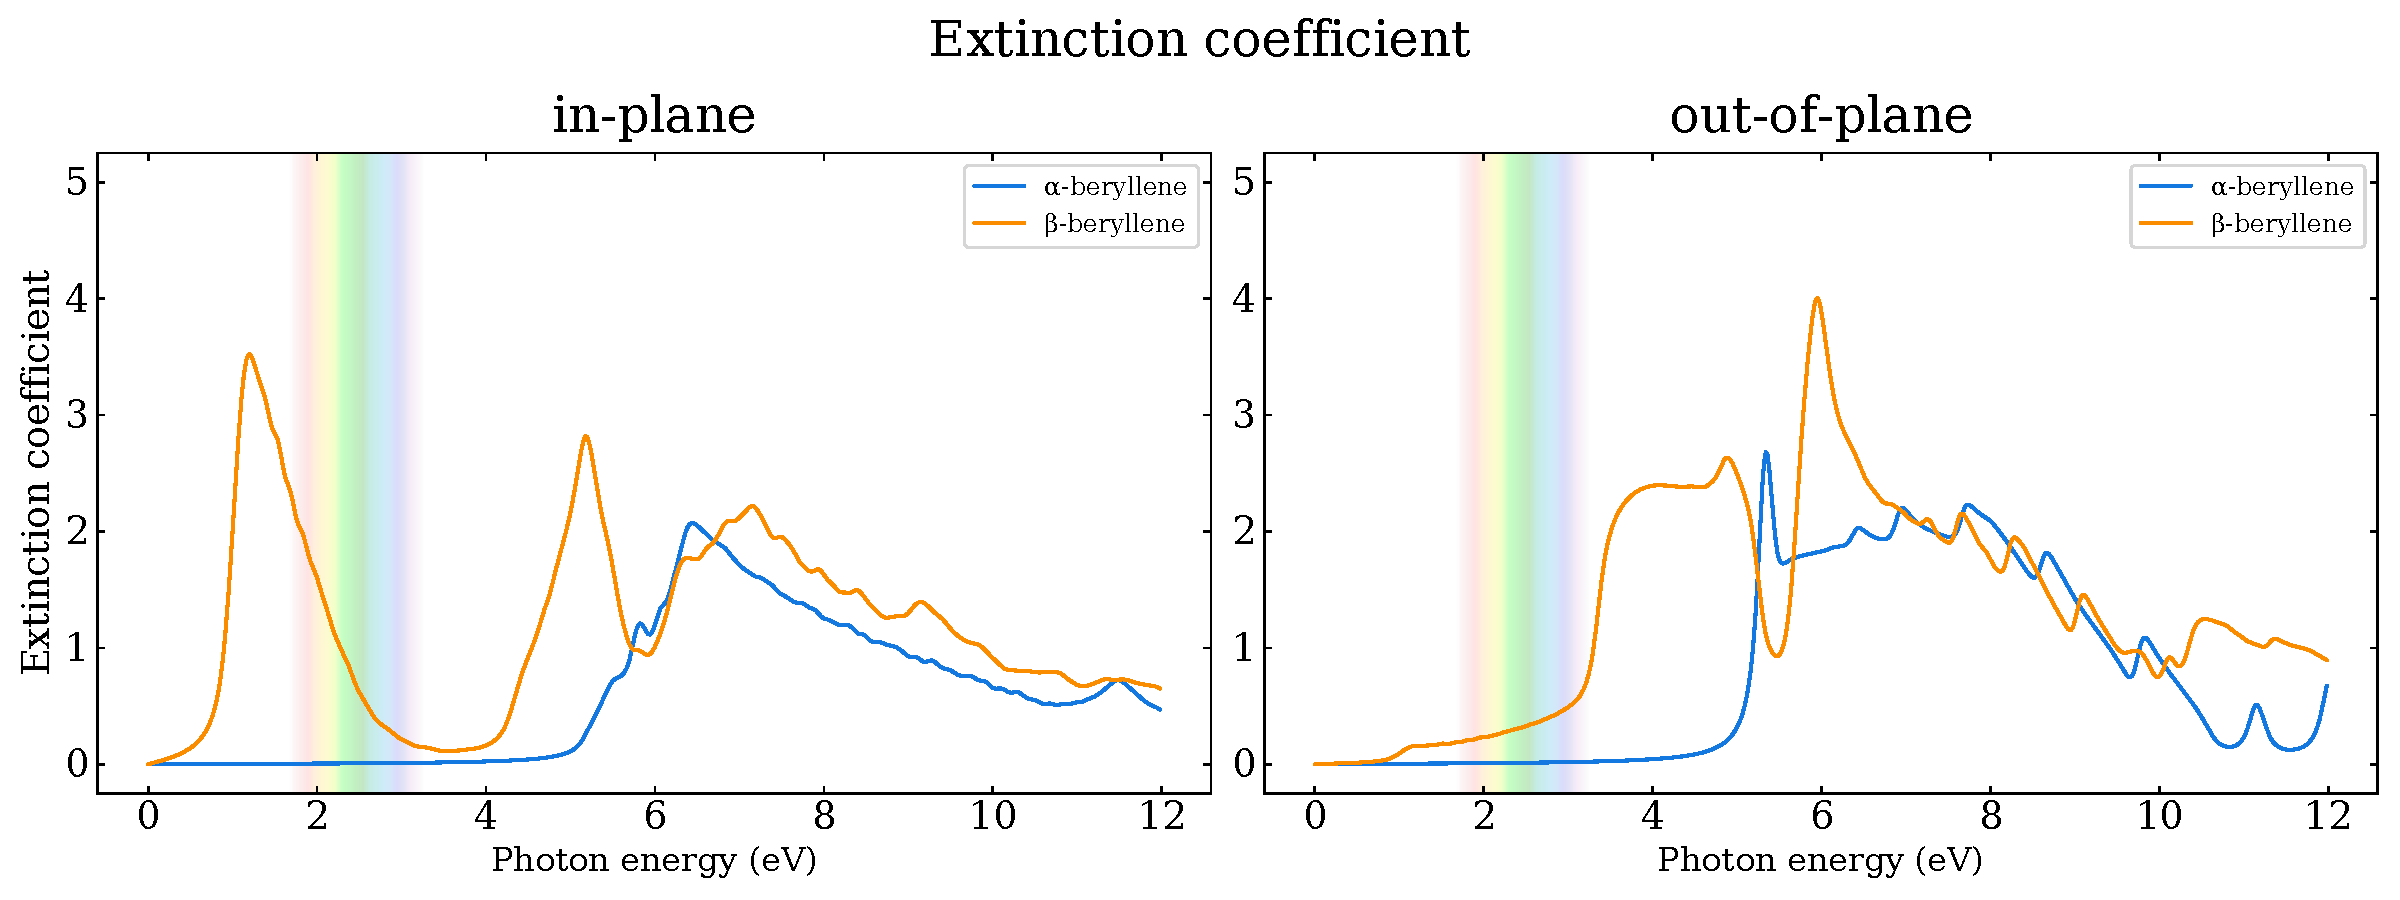
\includegraphics[width=0.80\linewidth]{figures_proj3/optics_alpha-beta_extinction_thesis.pdf}
\caption{Extinction coefficient of $\alpha$-beryllene and $\beta$-beryllene for the in-plane and out-of-plane directions as a function of photon energy.
The in-plane and out-of-plane curves correspond to the $xx$ and $zz$ components, respectively.}
\label{fig:proj3_alpha_beta_extinction}
\end{figure}

The corresponding reflectivity and energy-loss spectra show the same structural and directional contrast.
For reflectivity,
$\beta$-beryllene shows strong reflection in the low-energy and near-ultraviolet regions for in-plane polarization,
separated by a pronounced minimum.
In contrast,
$\alpha$-beryllene changes more smoothly and shows a broad intermediate-energy feature.
For out-of-plane polarization,
$\beta$-beryllene remains stronger over the low-energy range,
whereas $\alpha$-beryllene shows pronounced peaks in the ultraviolet region.

The in-plane energy-loss spectrum of $\beta$-beryllene has a visible-range local maximum of approximately 0.49
and a larger high-energy local maximum of approximately 1.34 near \qty{11.03}{\electronvolt}.
It reaches approximately 1.50 at the last available sample near \qty{11.98}{\electronvolt} while still rising;
this boundary value is not a resolved peak.
For out-of-plane response, $\alpha$-beryllene has a dominant loss maximum of approximately 8.88 near \qty{10.64}{\electronvolt},
substantially above the $\beta$ maximum of approximately 1.09 near \qty{9.95}{\electronvolt}.
These spectra describe the inverse dielectric response under the stated effective-thickness convention.

\subsubsection{Bulk hcp, bulk bcc, and trilayer cubic beryllene}
\label{3_optical_bulk_cubic}

We next compare the optical response of bulk hcp beryllium,
bulk bcc beryllium,
and trilayer cubic beryllene.
The real and imaginary parts of the dielectric function are shown in figure~\ref{fig:proj3_bulk_cubic_dielectric}.
The bulk hcp and bulk bcc structures show similar behaviour and weak directional dependence.
For both bulk structures,
the real part becomes negative above approximately \qty{4.5}{\electronvolt},
reaches a minimum around \qtyrange{5.5}{6.0}{\electronvolt},
and then rises smoothly toward zero around \qty{12}{\electronvolt}.
The imaginary part displays a broad low-energy feature up to approximately \qty{5.5}{\electronvolt},
indicating a wide range of allowed interband transitions.
It then decreases sharply around \qty{6}{\electronvolt},
coinciding with a minimum in the real part and a change in the inverse dielectric response.

For trilayer cubic beryllene,
the dielectric response is redistributed and becomes direction dependent relative to bulk bcc beryllium.
The largest imaginary dielectric features occur near \qty{3.74}{\electronvolt} in $xx$ and $yy$, with a value of approximately 19.75,
and near \qty{2.71}{\electronvolt} in $zz$, with a value of approximately 27.32.
The real part also develops direction-dependent sign changes.
These dielectric features do not coincide in general with absorption maxima, which also depend on the photon energy and the nonlinear relation between the dielectric function and the extinction coefficient.
Assignments to specific surface bands or transitions would require band- and matrix-element-resolved evidence.

\begin{figure}[!htbp]
\centering
    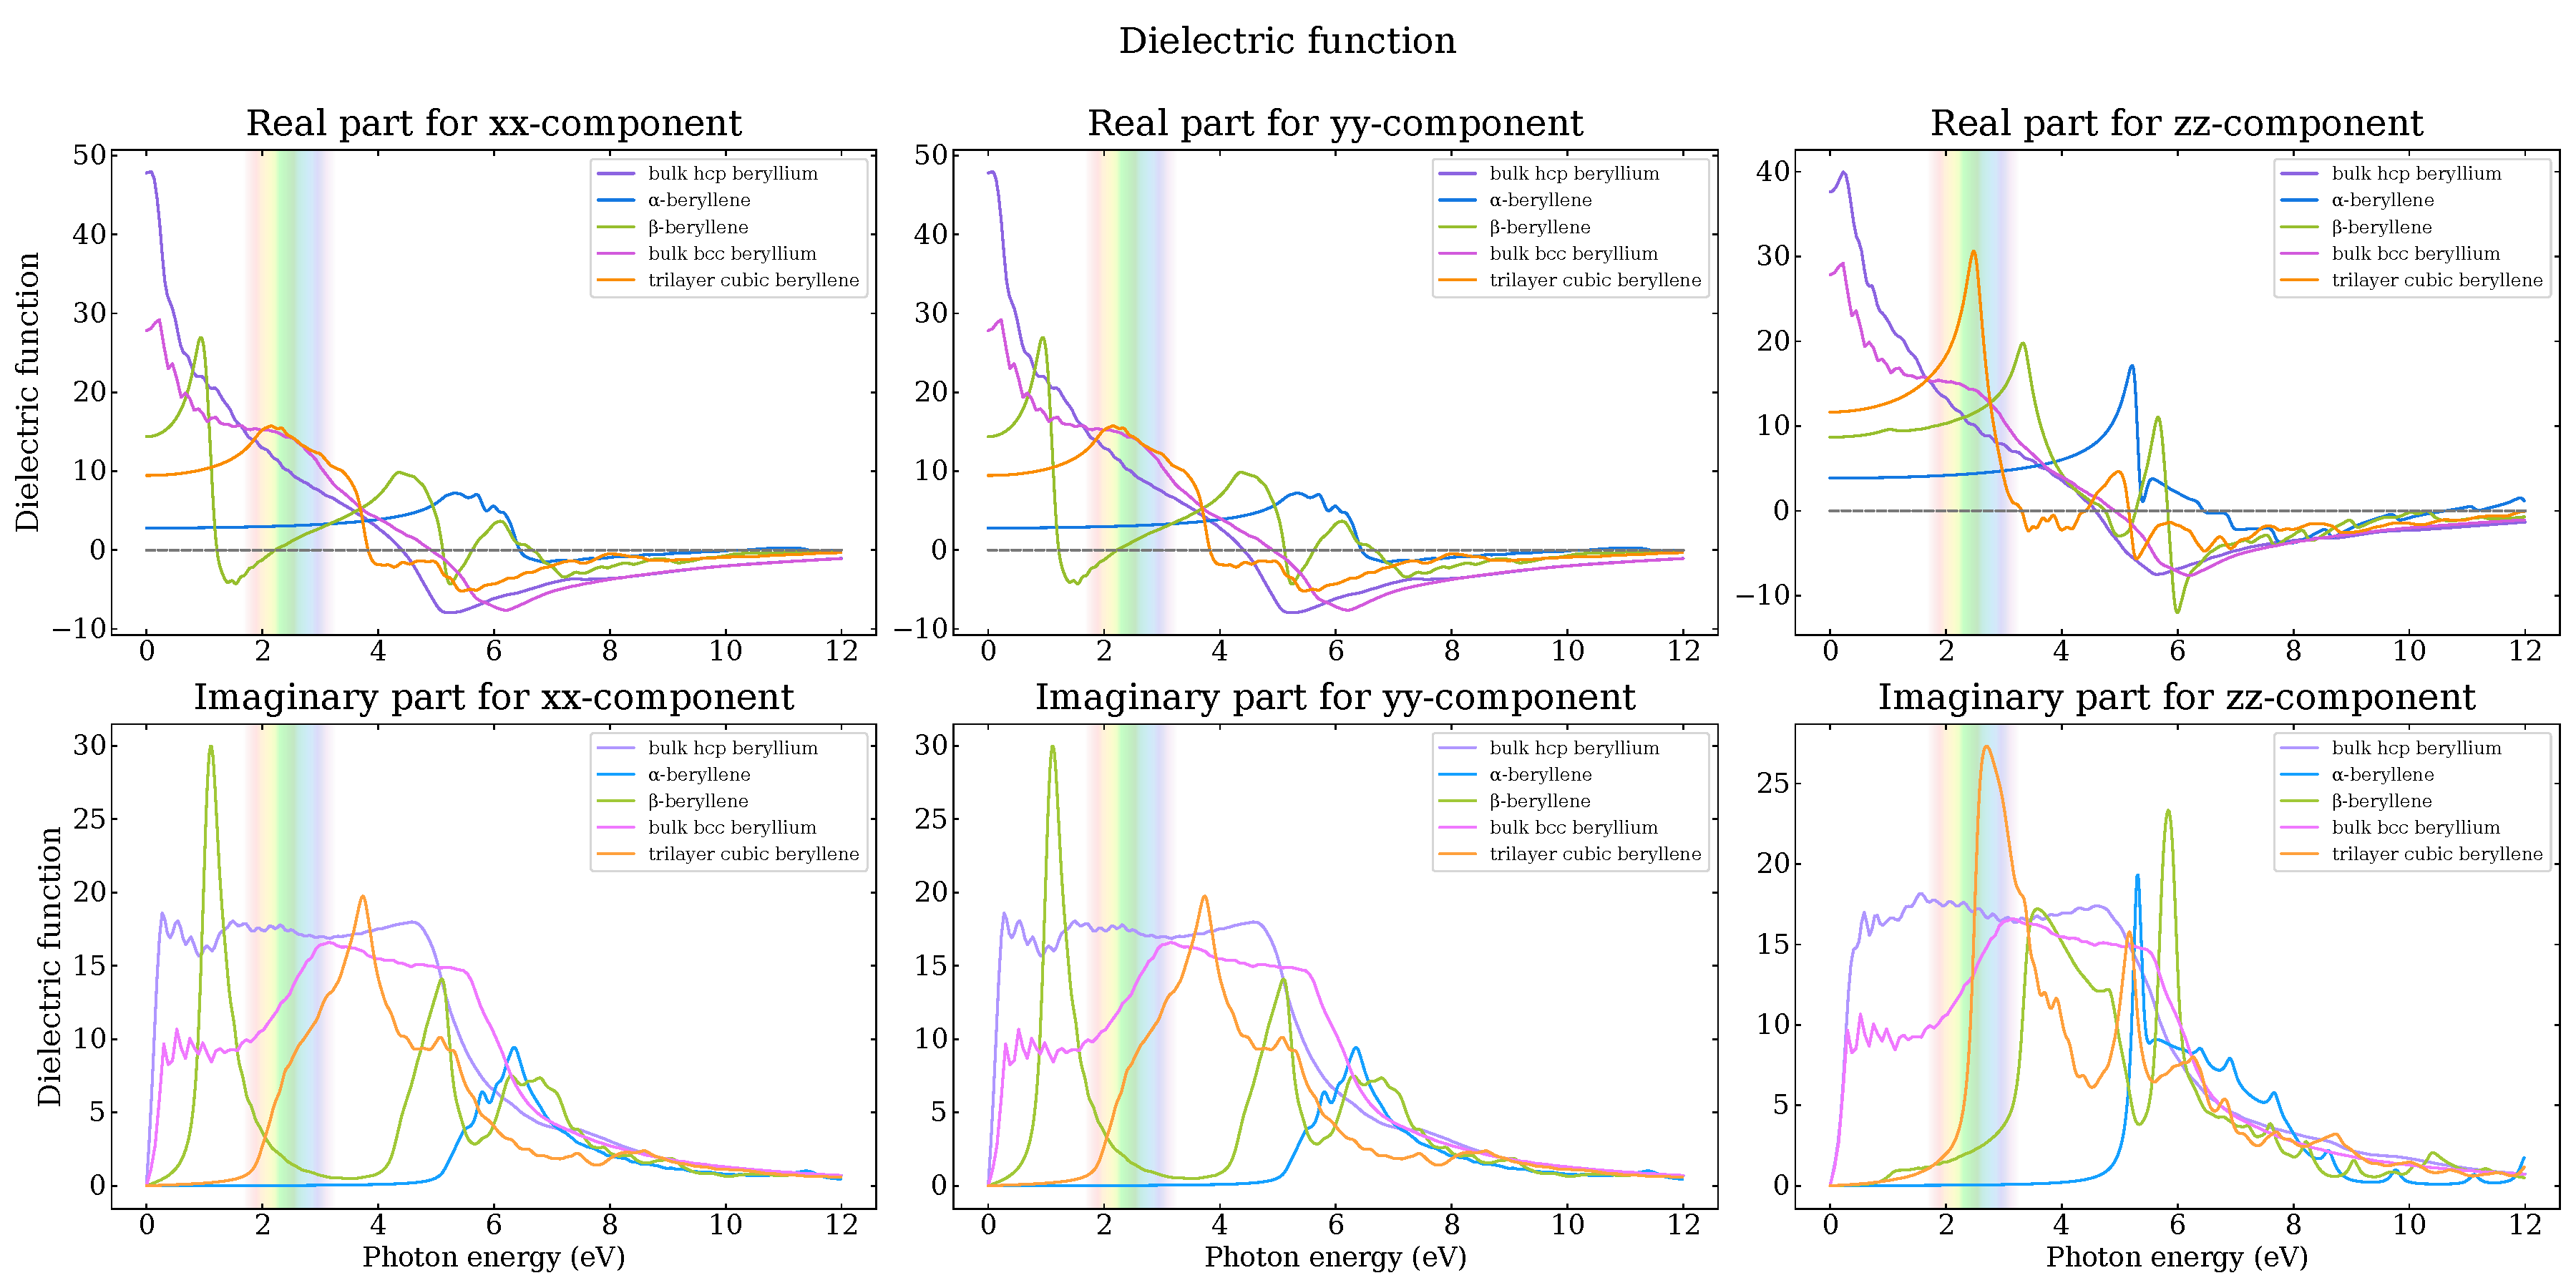
\includegraphics[width=0.95\linewidth]{figures_proj3/dielectric_pristine_thesis.pdf}
\caption{Real and imaginary parts of the dielectric function for bulk hcp beryllium,
bulk bcc beryllium,
$\alpha$-beryllene,
$\beta$-beryllene,
and trilayer cubic beryllene.
The spectra are shown for the $xx$,
$yy$,
and $zz$ components as functions of photon energy.}
\label{fig:proj3_bulk_cubic_dielectric}
\end{figure}

The absorption coefficient and energy-loss spectra are shown in figure~\ref{fig:proj3_bulk_cubic_abs_loss}.
Under the stated effective-thickness convention, trilayer cubic beryllene does not show a universal absorption enhancement relative to bulk bcc beryllium.
In the explicitly defined visible interval of \qtyrange{1.65}{3.26}{\electronvolt},
the trilayer $xx$ and $yy$ absorption is lower than bulk bcc at every available trilayer sample;
the bulk spectrum is linearly interpolated to the trilayer grid for this comparison.
The respective visible maxima are approximately \qty{0.0604}{\per\nano\metre} and \qty{0.0746}{\per\nano\metre}.
The trilayer $zz$ response exceeds the bulk value over only part of this interval.
Its strongest sampled absorption occurs near \qty{5.40}{\electronvolt} in $xx$ and $yy$,
and near \qty{5.25}{\electronvolt} in $zz$, with coefficients of approximately \qty{0.148}{\per\nano\metre} and \qty{0.166}{\per\nano\metre}, respectively.
These results show a redistribution of the effective interband response rather than enhanced absorption throughout the visible and near-ultraviolet regions.

The loss spectra also differ between directions and structures.
The low-energy $\beta$ in-plane feature and the high-energy $\alpha$ out-of-plane maximum are retained in the comparison.
The scalar loss features identify variations in the inverse dielectric response; they do not alone establish propagating plasmon modes.

\begin{figure}[!htbp]
\centering
    \adjustbox{valign=c}{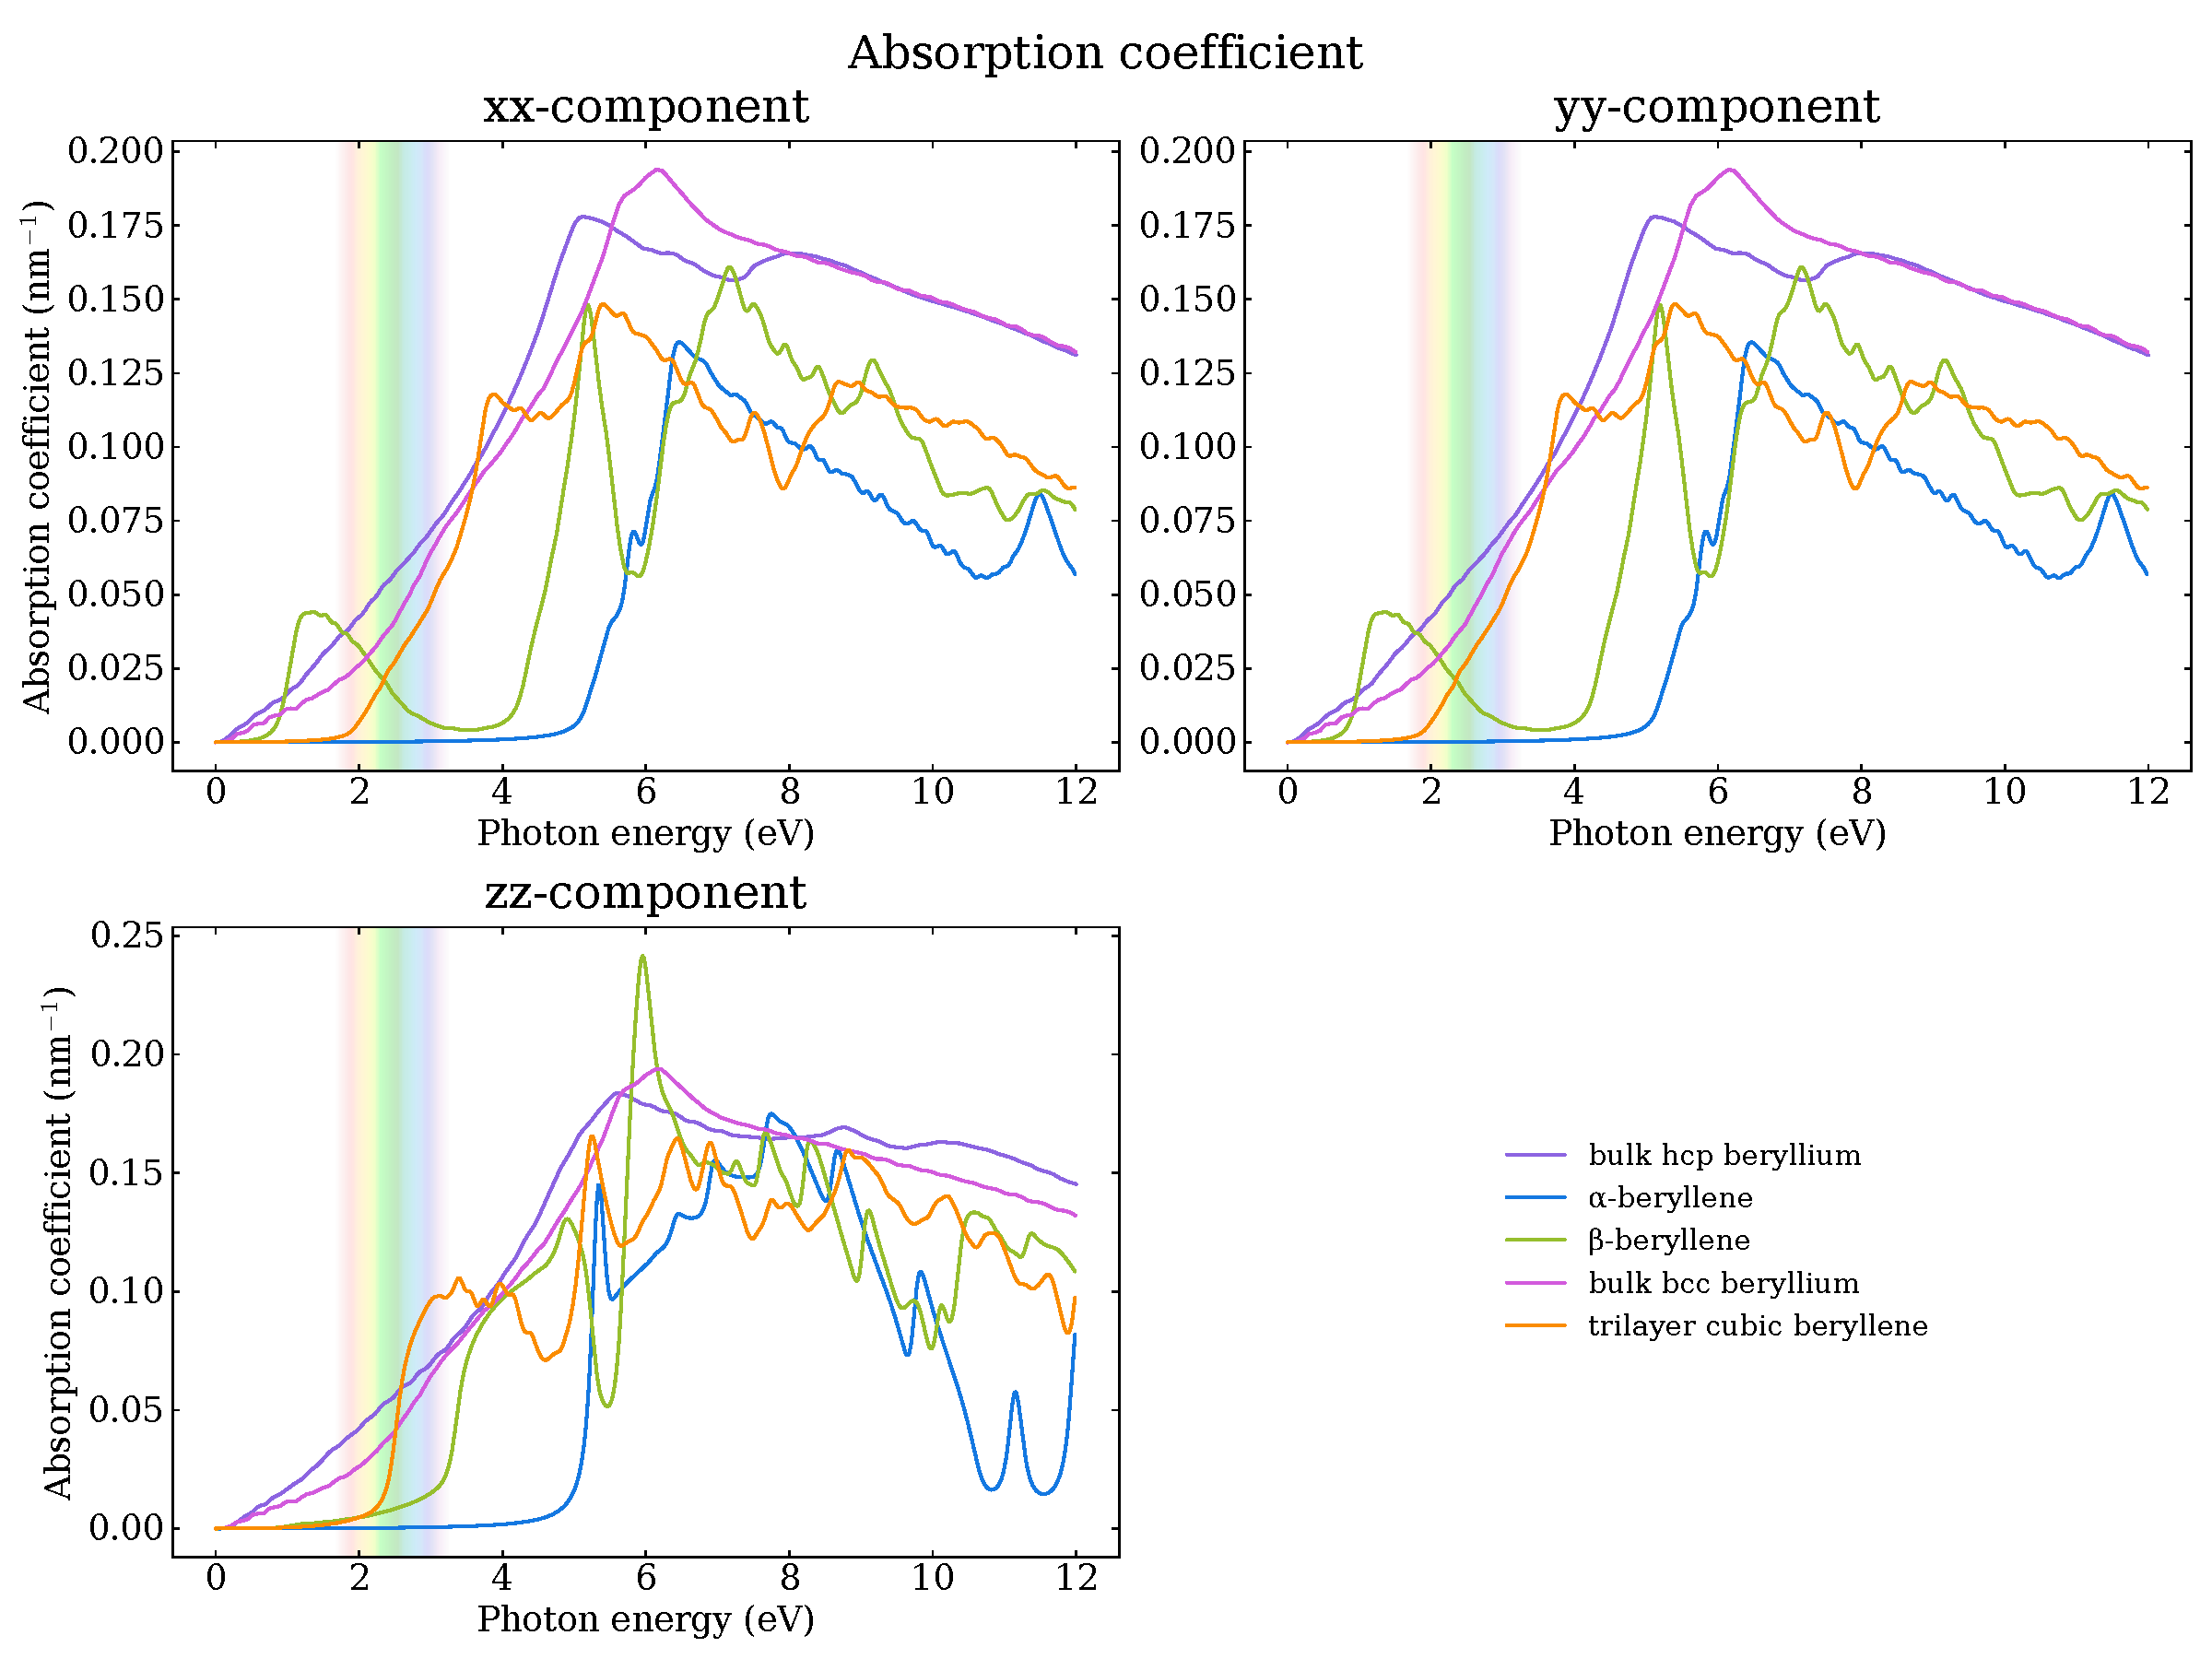
\includegraphics[width=0.80\linewidth]{figures_proj3/optics_pristine_absorption_thesis.pdf}}%
    \par\nointerlineskip
    \adjustbox{valign=c}{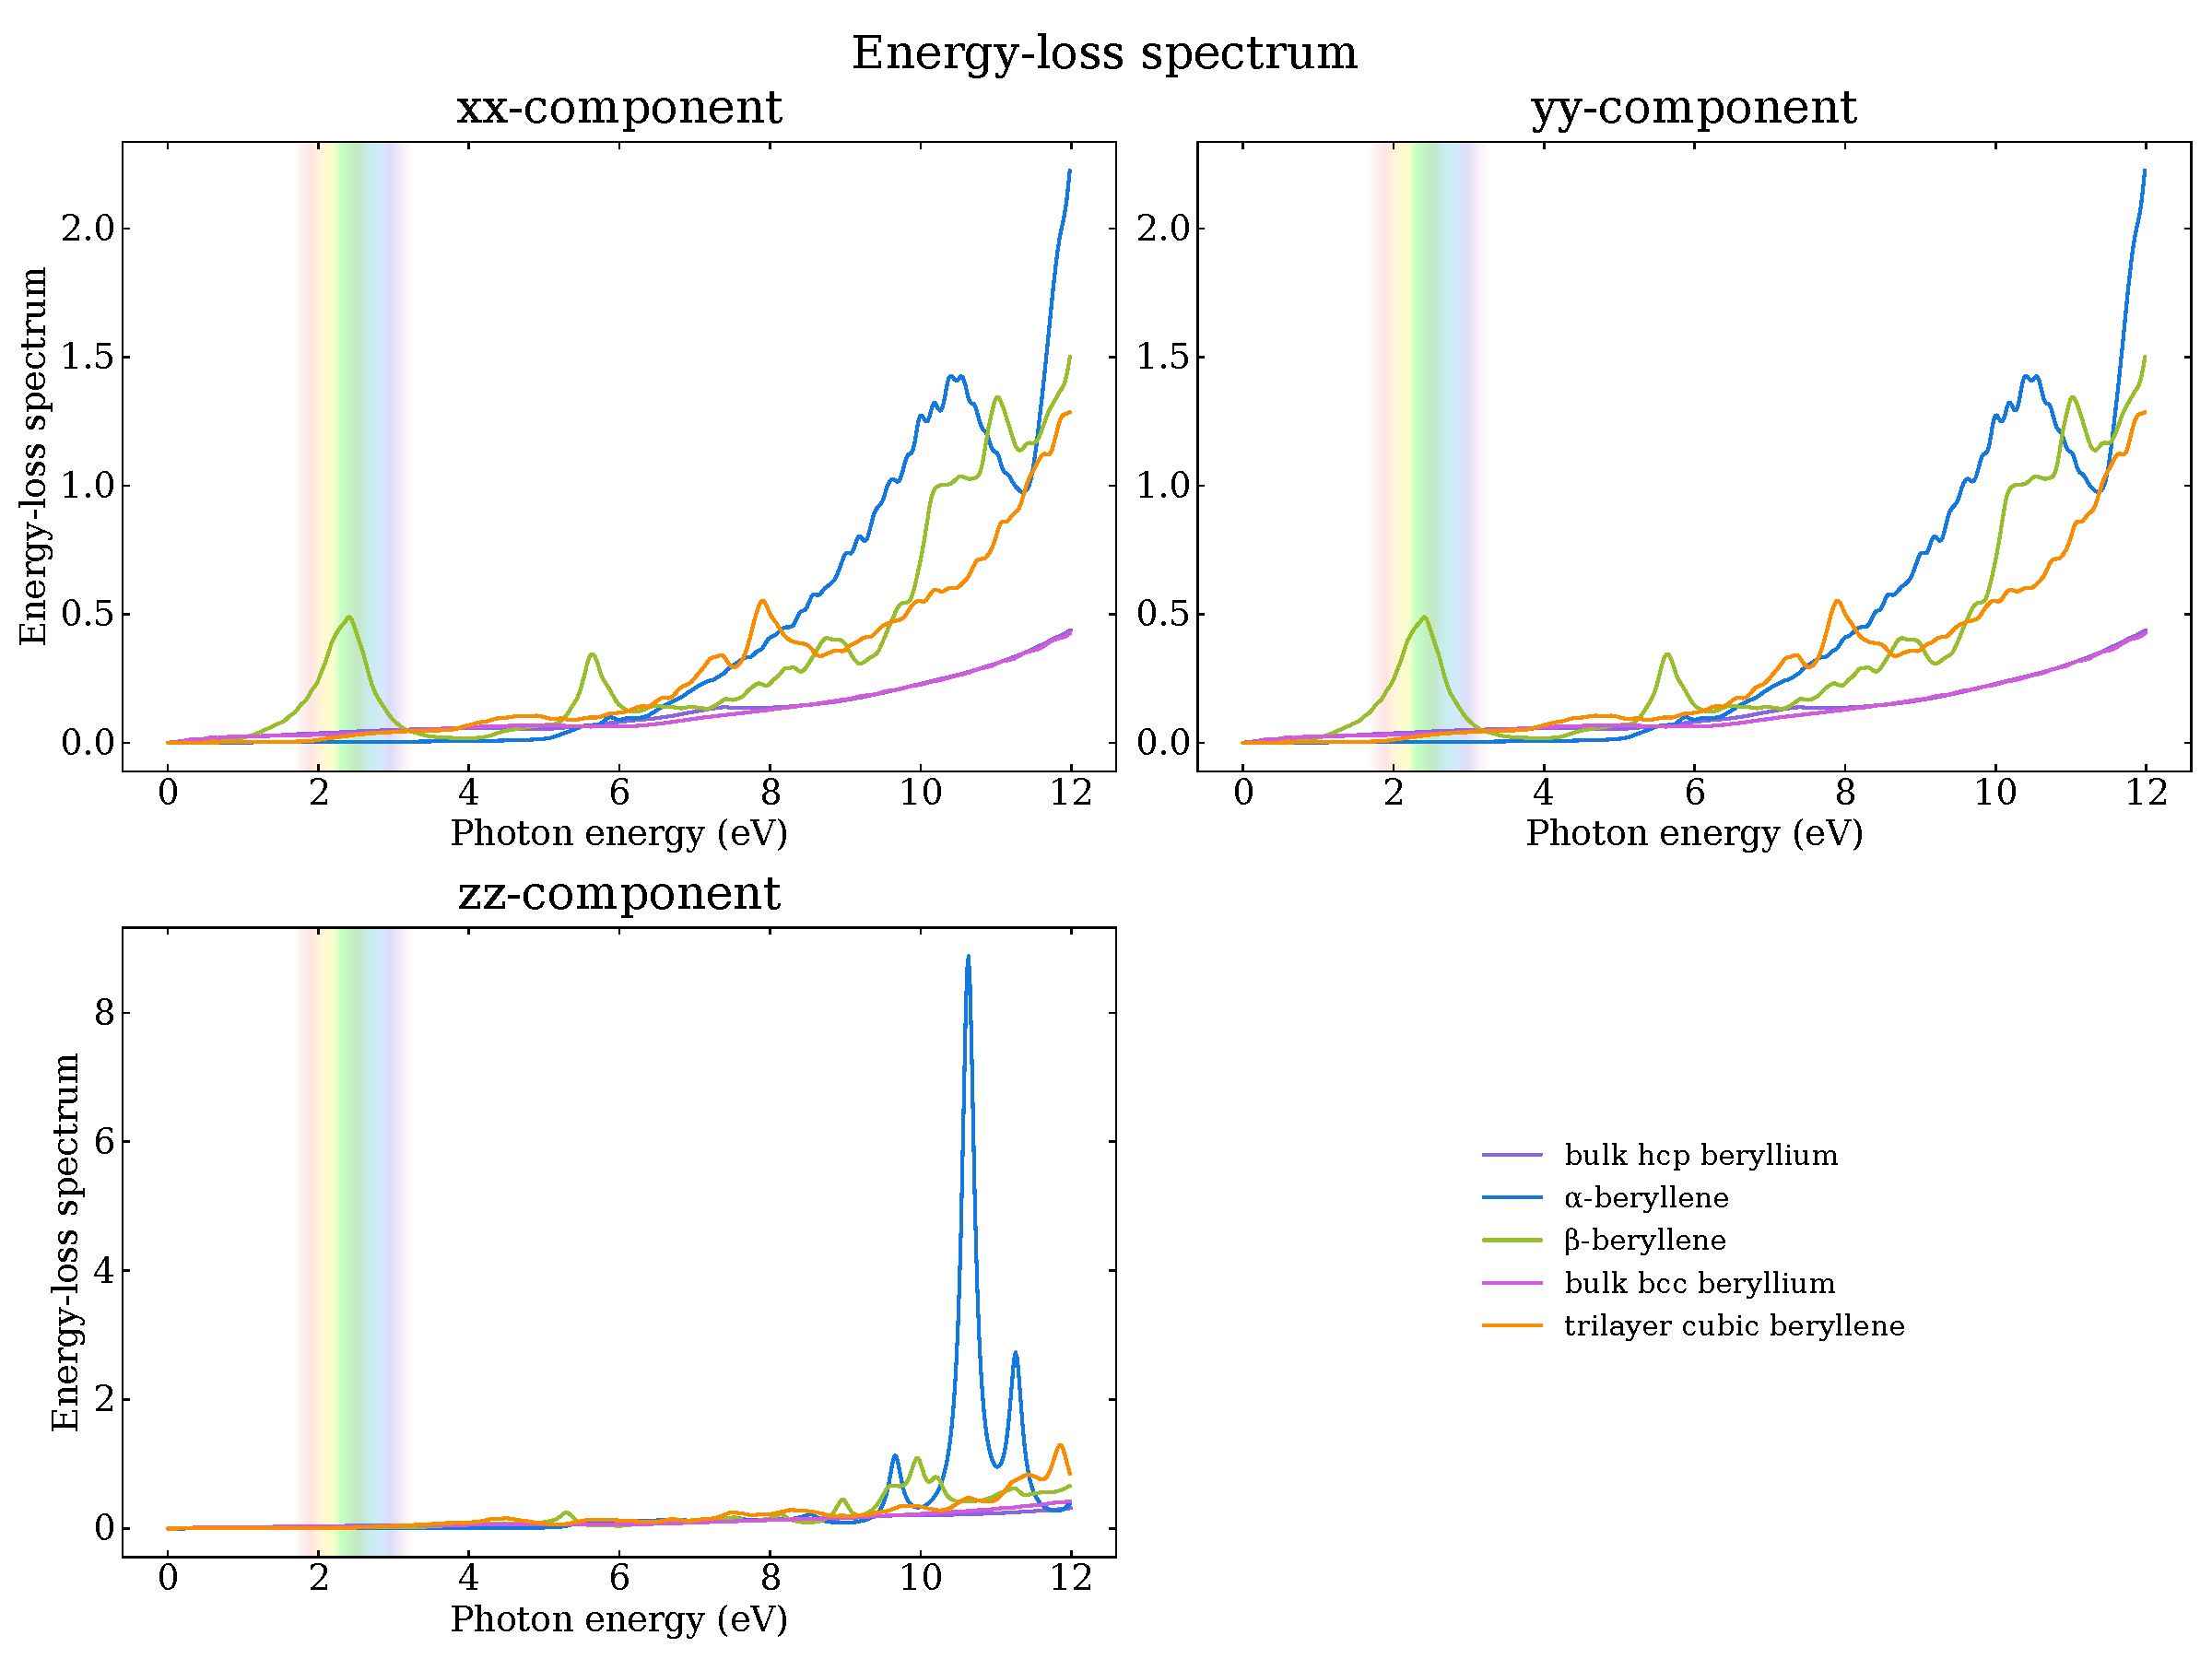
\includegraphics[width=0.80\linewidth]{figures_proj3/optics_pristine_energy-loss_thesis.pdf}}%
\caption{Absorption coefficient and energy-loss spectrum for bulk hcp beryllium,
bulk bcc beryllium,
$\alpha$-beryllene,
$\beta$-beryllene,
and trilayer cubic beryllene.
Upper: absorption coefficient ($\mathrm{nm}^{-1}$); Lower: energy-loss spectrum.
The spectra are shown for the $xx$,
$yy$,
and $zz$ components as functions of photon energy.}
\label{fig:proj3_bulk_cubic_abs_loss}
\end{figure}

\subsubsection{Hydrogen-functionalized beryllene structures}
\label{3_optical_hydrogenated_structures}

We now examine the effect of hydrogen adsorption on the optical properties of $\alpha$-beryllene and $\beta$-beryllene.
The real and imaginary parts of the dielectric function for the pristine and hydrogen-functionalized structures are shown in figure~\ref{fig:proj3_hydrogenated_dielectric}.

For $\alpha$-beryllene,
hydrogen adsorption changes the magnitude and spectral distribution of the effective dielectric response.
In $xx$ and $yy$, 2H-$\alpha$-beryllene has a real dielectric maximum of approximately 31.2 near \qty{4.91}{\electronvolt},
and its strongest imaginary dielectric feature is approximately 31.2 near \qty{5.59}{\electronvolt}.
The out-of-plane spectrum is different: its largest imaginary dielectric feature occurs near \qty{9.77}{\electronvolt}.
These comparisons retain the specified H/H surface-radius convention for the hydrogenated layer.
Changes in peak height therefore describe an effective response under that convention, not a thickness-independent measure of oscillator strength.

For $\beta$-beryllene,
single- and double-sided hydrogen adsorption redistribute the dielectric response and change its directional dependence.
Double-sided adsorption produces distinct spectra in all three Cartesian components.
The strongest imaginary dielectric features occur near \qty{6.59}{\electronvolt} in $xx$,
\qty{9.26}{\electronvolt} in $yy$ and \qty{8.24}{\electronvolt} in $zz$,
with values of approximately 14.96, 7.68 and 14.97, respectively.
The first real-part sign changes occur near \qty{6.64}{\electronvolt}, \qty{9.32}{\electronvolt} and \qty{8.10}{\electronvolt}, respectively.
Thus, increasing hydrogen coverage changes the spectral distribution and in-plane anisotropy;
it does not produce a common peak energy, a common zero crossing, or a monotonic enhancement in every component.
The imaginary dielectric peaks should also be distinguished from maxima of the derived absorption coefficient.

\begin{figure}[!htbp]
\centering
    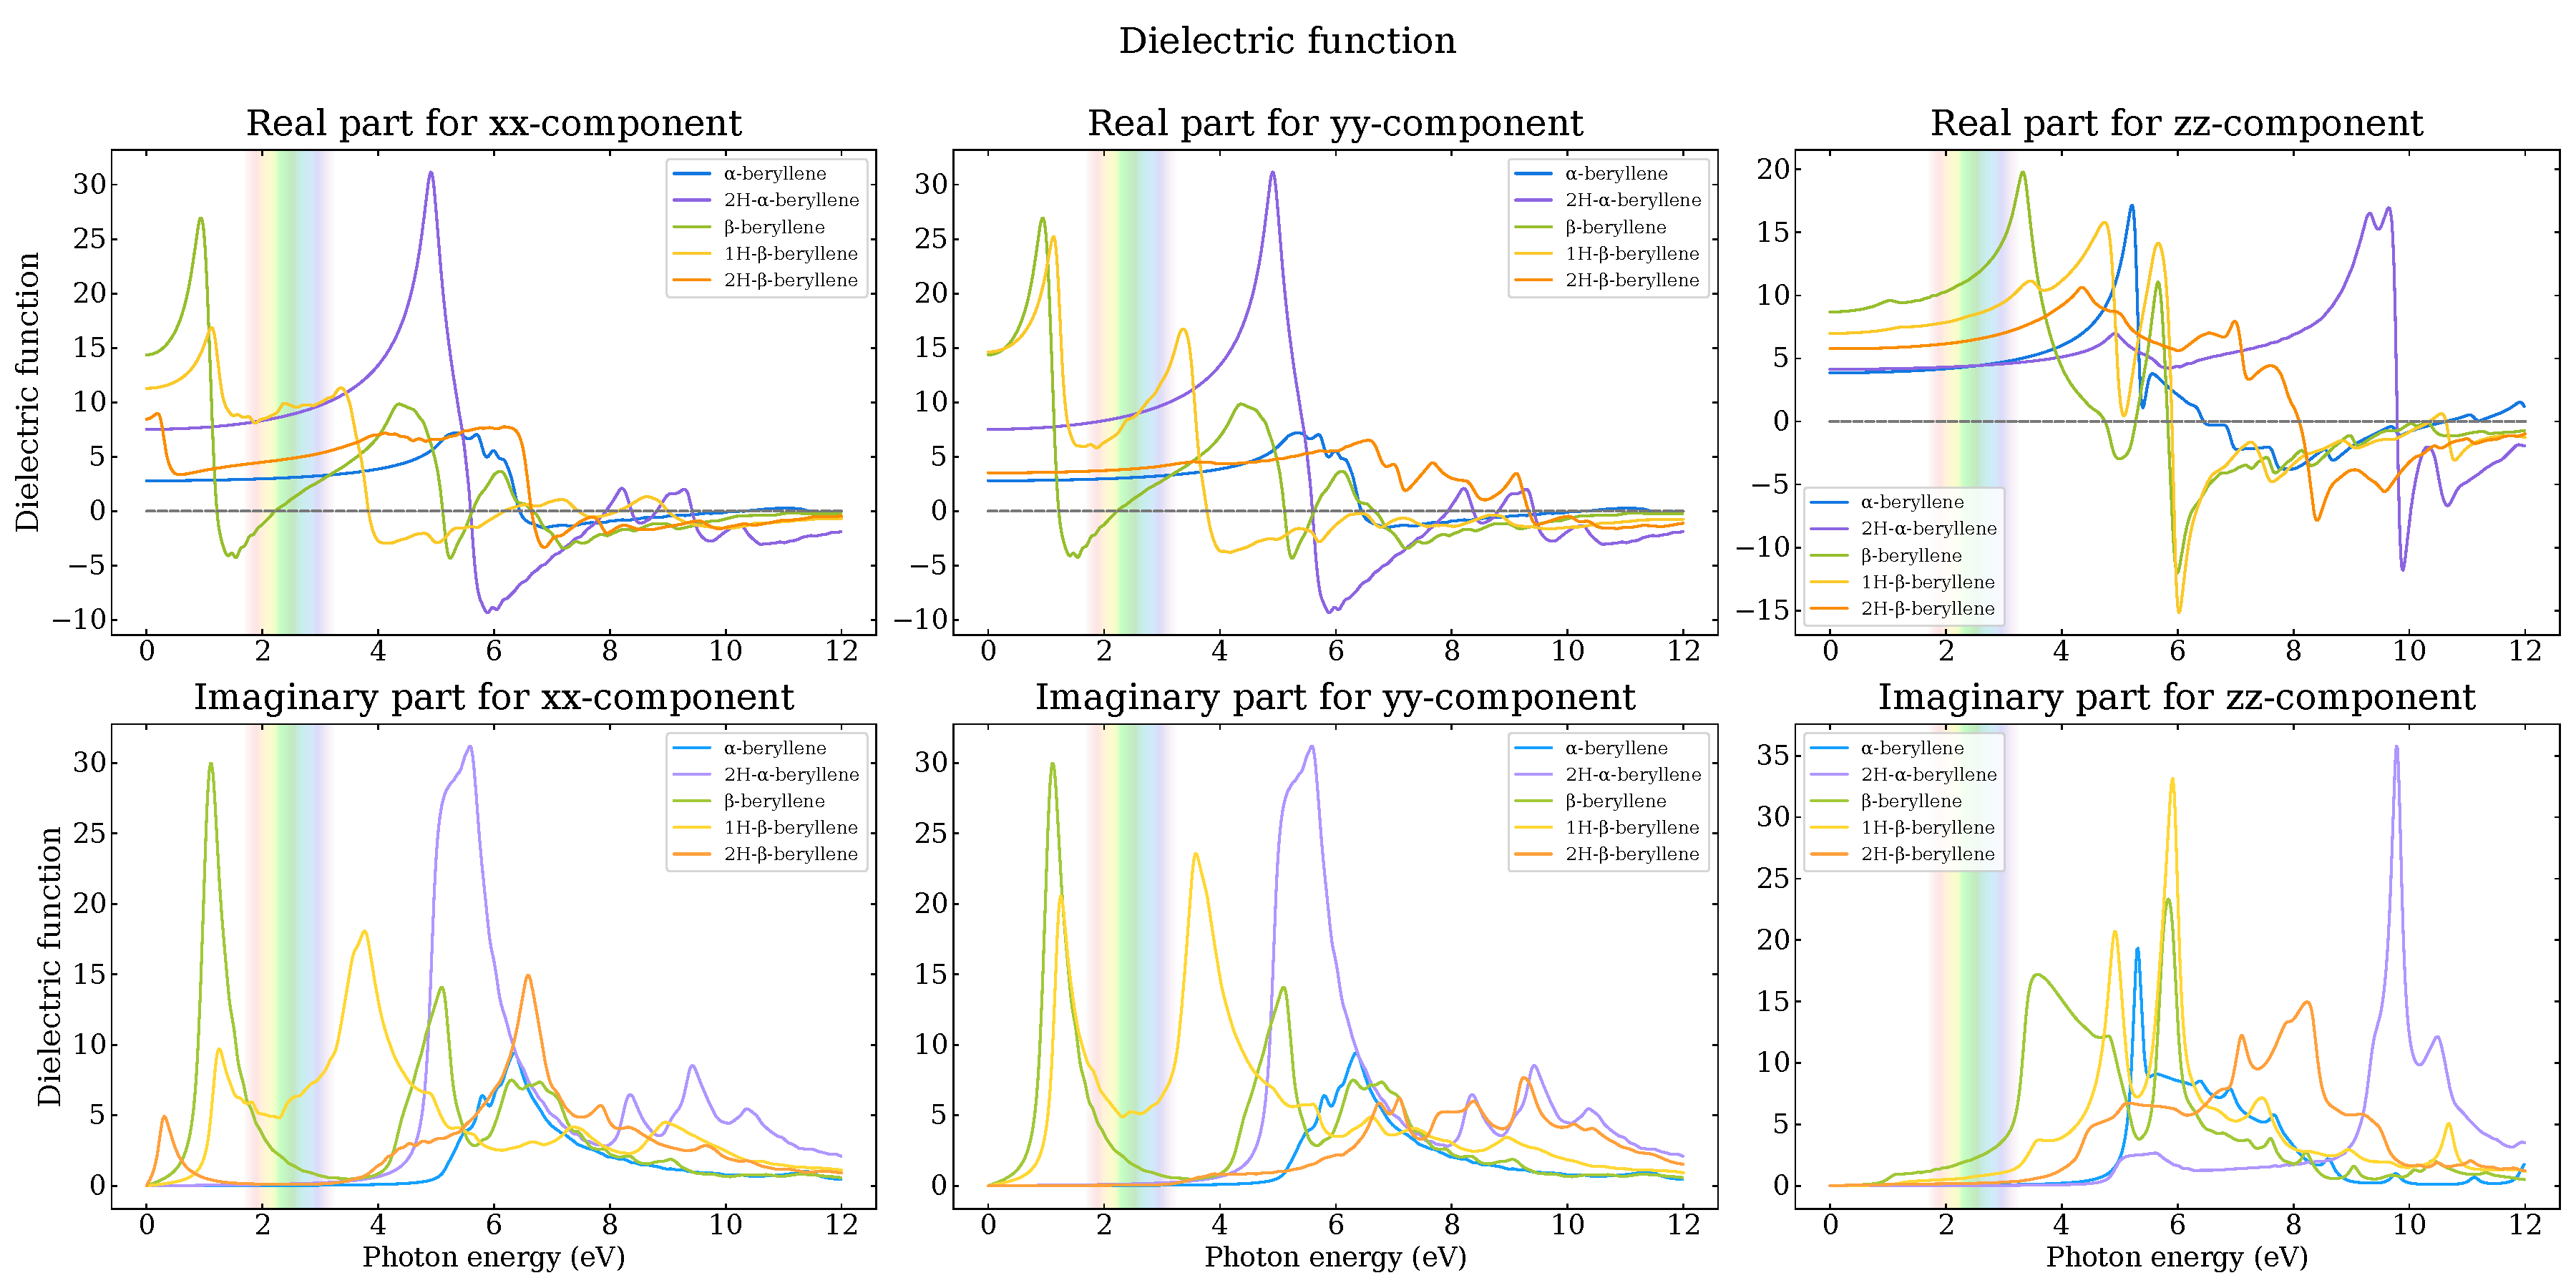
\includegraphics[width=1\linewidth]{figures_proj3/dielectric_hydrogenated_thesis.pdf}
\caption{Real and imaginary parts of the dielectric function for pristine and hydrogen-functionalized $\alpha$- and $\beta$-beryllene structures.
The spectra are shown for the $xx$,
$yy$,
and $zz$ components as functions of photon energy.}
\label{fig:proj3_hydrogenated_dielectric}
\end{figure}

The corresponding absorption coefficient and energy-loss spectra are shown in figure~\ref{fig:proj3_hydrogenated_abs_loss}.
For $\alpha$-beryllene, hydrogen adsorption produces a strongly direction-dependent redistribution of absorption.
The $xx$ and $yy$ coefficients increase over the sampled visible interval,
but the 2H-$\alpha$ visible maximum is only approximately \qty{0.00137}{\per\nano\metre}, much smaller than its ultraviolet maximum near \qty{5.71}{\electronvolt}.
The $zz$ coefficient instead decreases throughout the sampled \qtyrange{1.65}{4.13}{\electronvolt} interval,
and its strongest peak occurs near \qty{9.83}{\electronvolt}.
For 2H-$\beta$-beryllene, the strongest sampled absorption peaks occur near \qty{6.75}{\electronvolt} in $xx$,
\qty{9.39}{\electronvolt} in $yy$ and \qty{8.36}{\electronvolt} in $zz$.
The loss spectra likewise change with hydrogen coverage and direction.
These results establish changes in the calculated interband and inverse dielectric response;
weak low-energy tails under finite numerical broadening are not evidence of a sharply defined absorption onset or strong visible absorption.

\begin{figure}[!htbp]
\centering
    \adjustbox{valign=c}{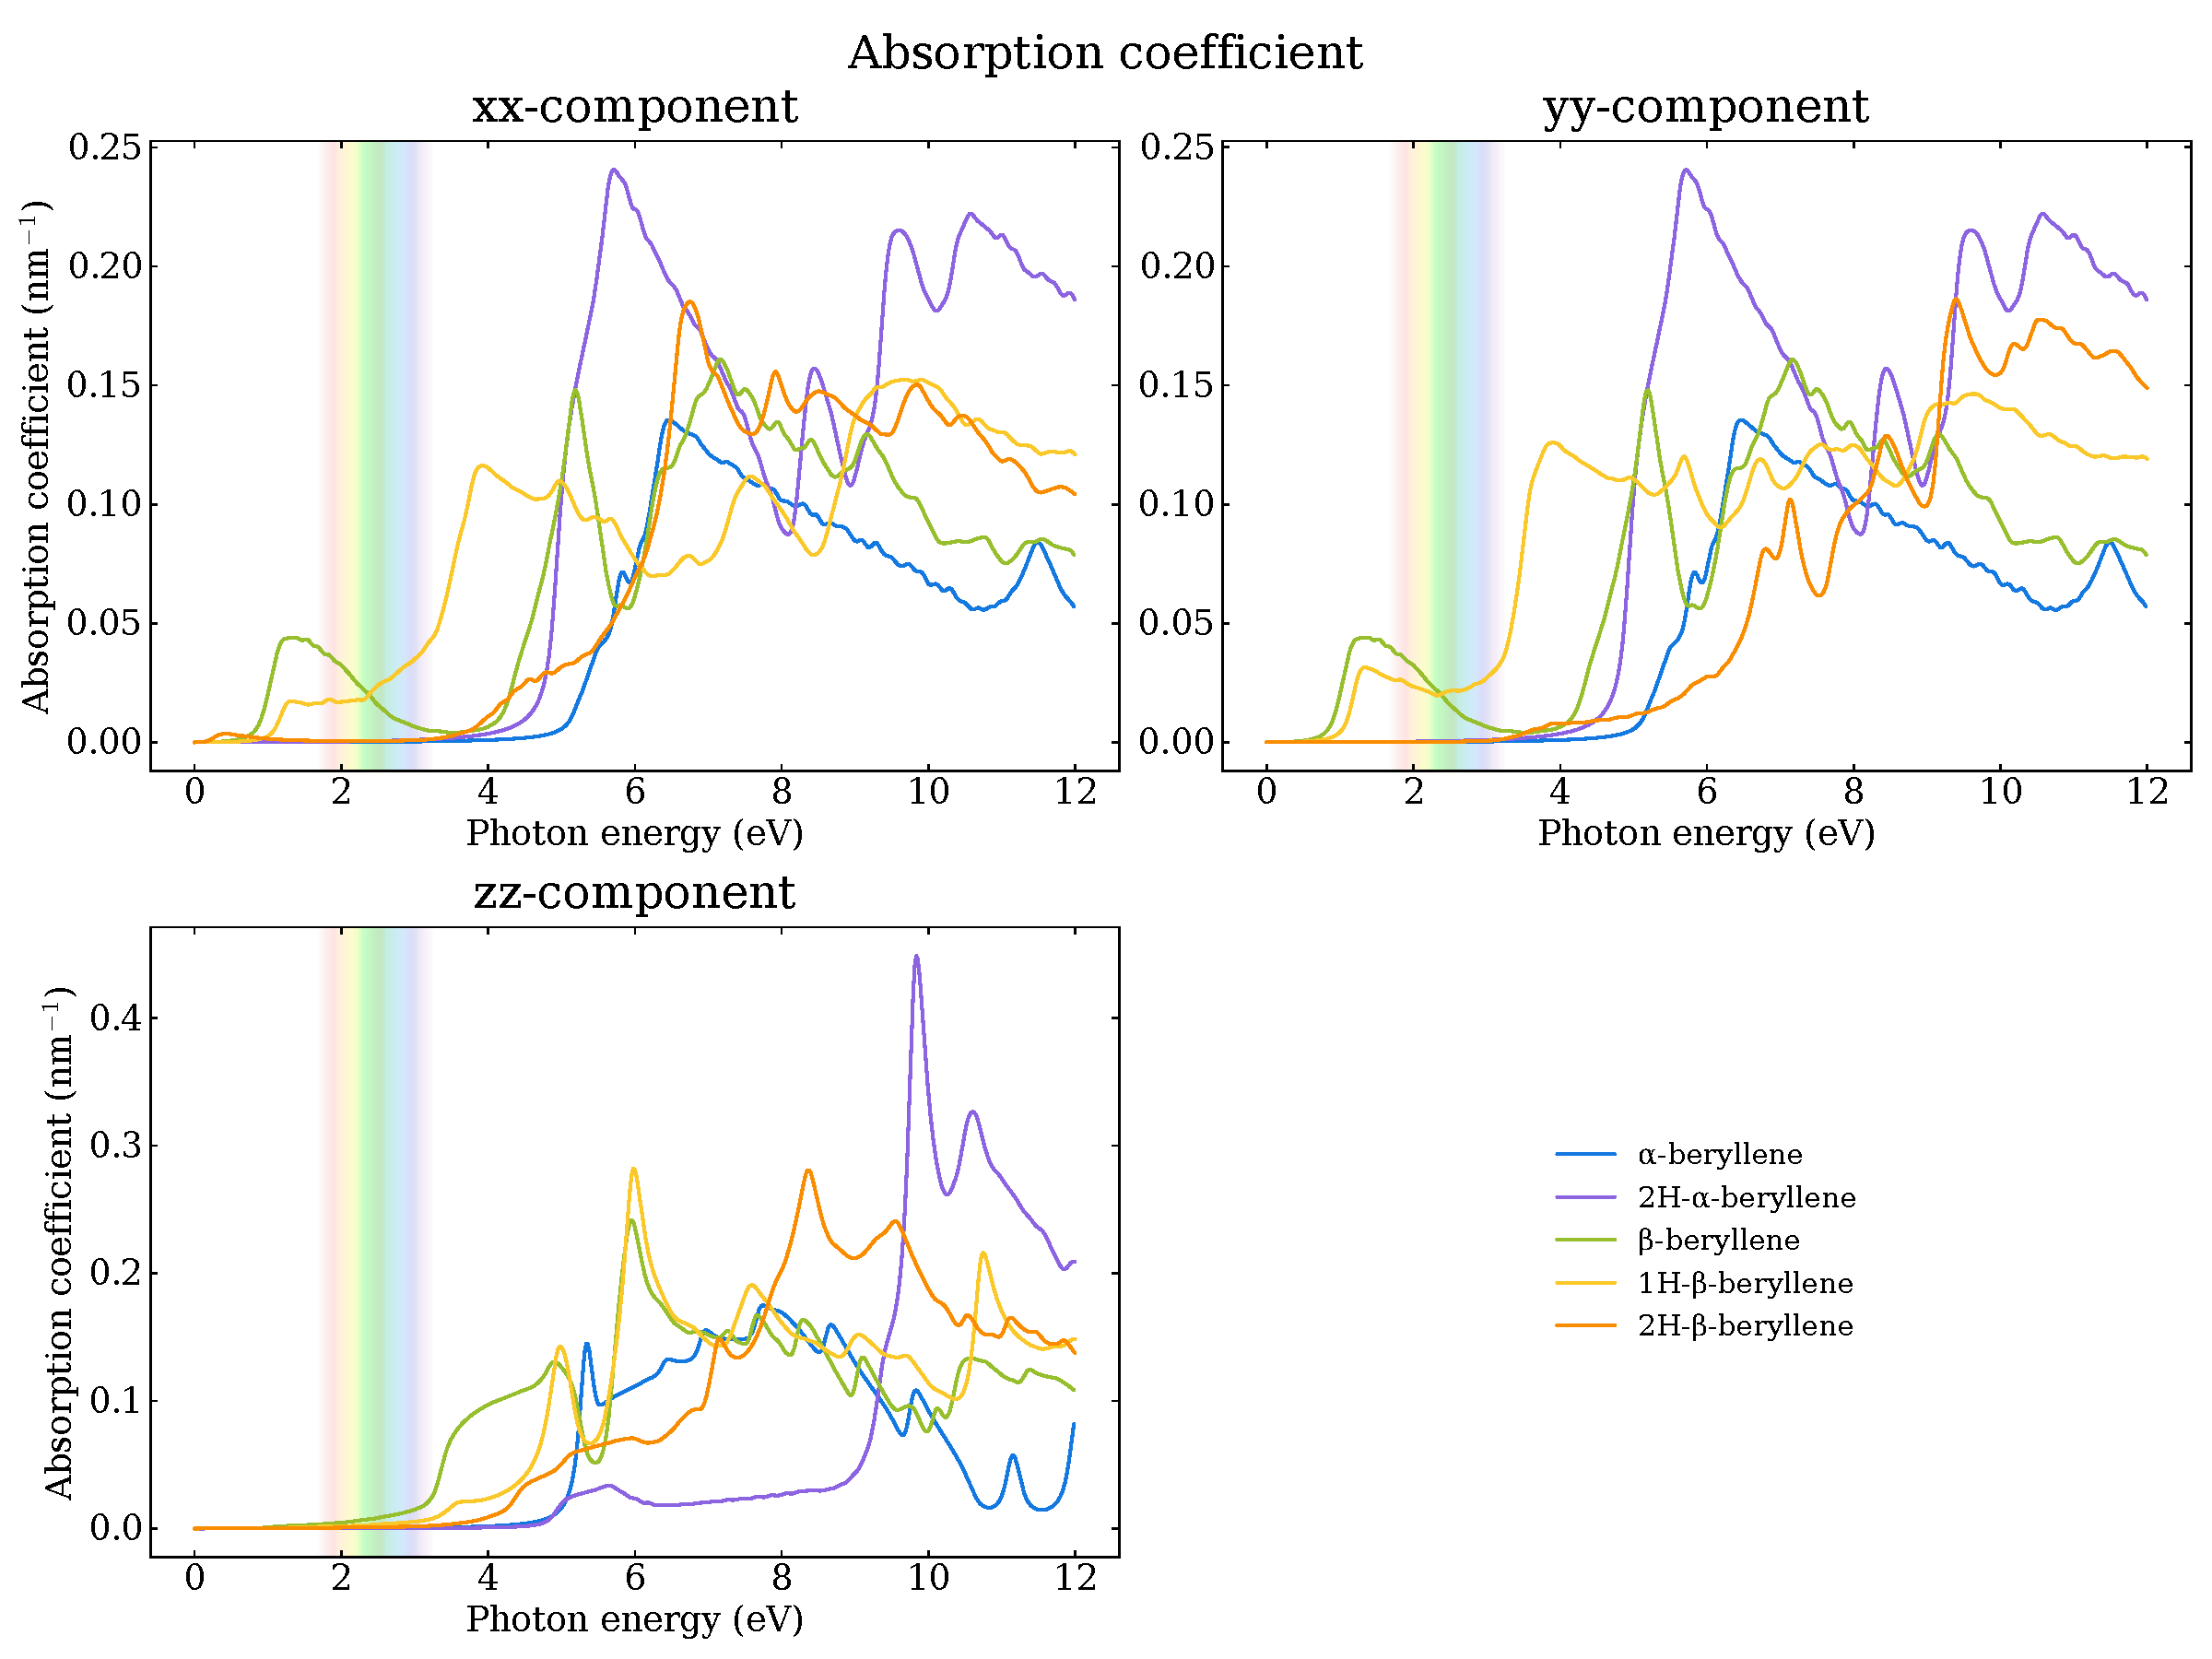
\includegraphics[width=0.80\linewidth]{figures_proj3/optics_hydrogenated_absorption_thesis.pdf}}%
    \par\nointerlineskip
    \adjustbox{valign=c}{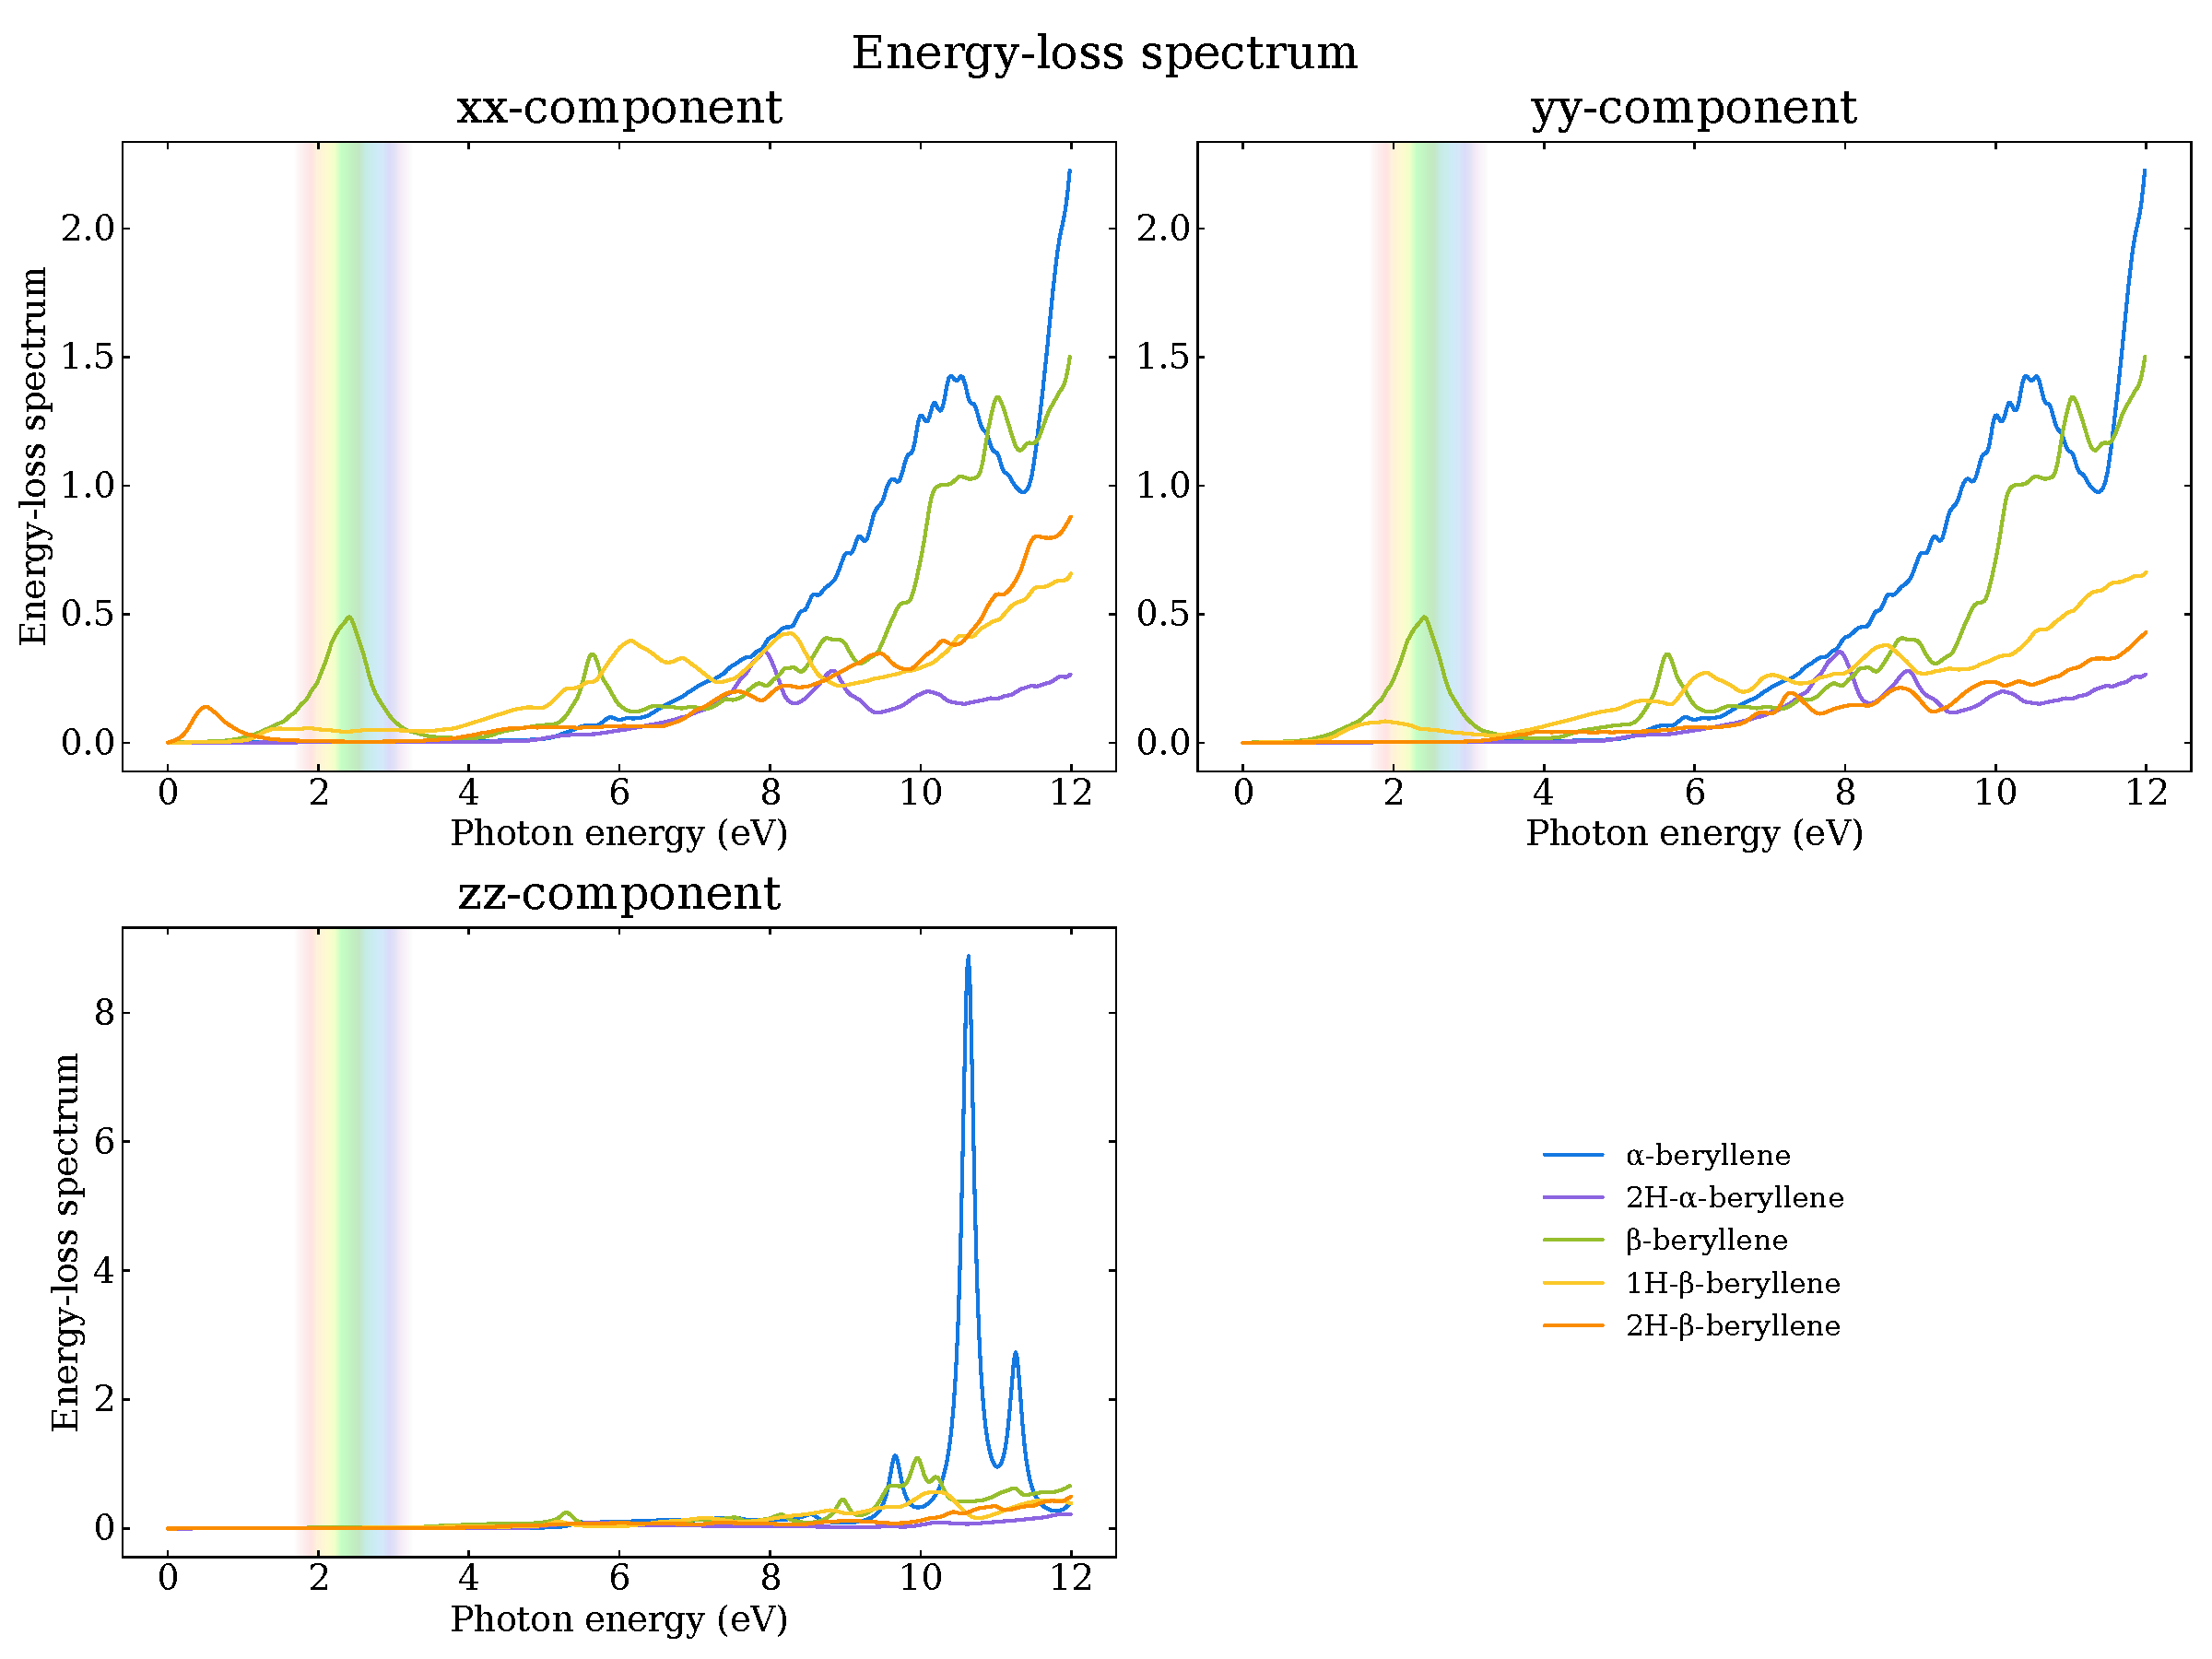
\includegraphics[width=0.80\linewidth]{figures_proj3/optics_hydrogenated_energy-loss_thesis.pdf}}%
\caption{Absorption coefficient and energy-loss spectrum for pristine and hydrogen-functionalized $\alpha$- and $\beta$-beryllene structures.
Upper: absorption coefficient ($\mathrm{nm}^{-1}$); Lower: energy-loss spectrum.
The spectra are shown for the $xx$,
$yy$,
and $zz$ components as functions of photon energy.}
\label{fig:proj3_hydrogenated_abs_loss}
\end{figure}

These results show that both dimensionality and hydrogen functionalization redistribute the effective interband optical response of beryllene.
Pristine $\alpha$- and $\beta$-beryllene exhibit pronounced anisotropy, while trilayer cubic beryllene and the hydrogenated phases enhance some components and reduce others.
The comparisons depend on the stated thickness convention and do not include a Drude intraband contribution.

\section{Conclusions}
\label{3_conclusions}

In this chapter,
we investigated the structural stability,
electronic structure,
optical response,
and topological properties of pristine and hydrogen-functionalized two-dimensional beryllium phases using first-principles density functional theory calculations.
Alongside the previously reported $\alpha$- and $\beta$-beryllene structures,
we identified a dynamically stable trilayer cubic beryllene phase.
The phonon dispersion calculations also confirm the dynamical stability of 2H-$\alpha$-beryllene and 1H-$\beta$-beryllene.
2H-$\beta$-beryllene has a harmonic soft mode,
but this mode is stabilized by its strong anharmonicity and quantum fluctuations.
The molecular dynamics simulations further support the finite-temperature stability of these hydrogen-functionalized structures.

Hydrogen functionalization substantially modifies the structural and electronic properties of beryllene.
In particular,
it transforms metallic $\alpha$-beryllene into 2H-$\alpha$-beryllene,
a wide-gap semiconductor with an HSE06 band gap of \qty{6.00}{\electronvolt},
whereas the hydrogen-functionalized $\beta$-based structures retain metallic behaviour.
The calculated adsorption energies show that hydrogen adsorption is exothermic with respect to molecular hydrogen.
Including zero-point and thermal contributions,
only 2H-$\alpha$-beryllene is thermodynamically stable against \ce{H2} release under ambient conditions,
whereas 2H-$\beta$-beryllene requires an elevated \ce{H2} pressure and 1H-$\beta$-beryllene can exist only as a kinetically trapped phase.

The calculated optical properties show a direction-dependent redistribution of the effective interband response after dimensional reduction and hydrogen functionalization.
Pristine $\alpha$- and $\beta$-beryllene exhibit pronounced anisotropy and distinct loss features.
The absorption of trilayer cubic beryllene does not exceed that of bulk bcc beryllium throughout the visible range or in all directions,
and hydrogen adsorption enhances some components while reducing others.
These comparisons use the stated effective-thickness convention and exclude a Drude intraband contribution.

Parity analysis of the spin-orbit-coupled electronic states confirms the previously reported non-trivial topology of $\alpha$-beryllene and the trivial topology of $\beta$-beryllene.
Trilayer cubic beryllene also has a non-trivial $Z_2$ invariant,
whereas all hydrogen-functionalized structures are trivial.
Since the non-trivial subspaces of these metallic phases are isolated only by spin-orbit gaps of approximately \qty{1}{\milli\electronvolt} above the Fermi level,
these indices are conditional screening results for band inversions rather than quantum spin Hall states.
Together with the previously reported superconducting behaviour of beryllene~\cite{li2023coexistence},
these results identify two-dimensional beryllium as an elemental platform in which structural design and hydrogen functionalization can tune the electronic,
optical,
and topological properties.
